\RequirePackage[hyphens]{url}

\documentclass[longtitle]{elsarticle}


%
% Packages
%

\usepackage[utf8]{inputenc}
\usepackage[T1]{fontenc}
\usepackage{lmodern}
\usepackage{listings}
\usepackage{amsmath}
\allowdisplaybreaks
\usepackage{amsfonts}
\usepackage{amstext}
\usepackage{amssymb}
\usepackage{amsthm}
\usepackage{empheq}
\usepackage{cases}
\usepackage{anyfontsize}
\usepackage{enumitem}
\usepackage{pdfpages}
\usepackage{fourier}	% Style
\usepackage{bm}
\usepackage{epstopdf}
\usepackage{lipsum}
\usepackage[top=3cm, bottom=3cm, left=2cm, right=2cm, scale=0.75]{geometry}	% Set the margins
\usepackage{fancyhdr}
\usepackage[letterspace=150]{microtype}
\usepackage{textcomp}
\usepackage{gensymb}
\usepackage{booktabs}
\usepackage{amsmath,etoolbox}
\usepackage{mathtools}
\usepackage{anyfontsize}
\usepackage{graphicx}
\usepackage{epstopdf}
\usepackage{float}
\usepackage{subfig}
\usepackage[labelfont=bf,labelsep=period,font=small]{caption}
\usepackage{newunicodechar}
\usepackage{nicefrac}	% For diagonal fractions
\usepackage{bbm}
\usepackage{csvsimple}

% Set header and footer
\usepackage{fancyhdr}

% Packages needed for tables
\usepackage{longtable}
\usepackage{multicol}
\usepackage{multirow}
\usepackage{array}

\PassOptionsToPackage{hyphens}{url}\usepackage{hyperref}
\usepackage{breakurl}
\usepackage{url}

% To put footnotes at the bottom of the page
\usepackage[bottom]{footmisc}

\usepackage{empheq}

\usepackage{tikz}

% Default fixed font does not support bold face
\DeclareFixedFont{\ttb}{T1}{txtt}{bx}{n}{10.25} % for bold
\DeclareFixedFont{\ttm}{T1}{txtt}{m}{n}{10.25}  % for normal

% Custom colors
\usepackage{color}
\definecolor{deepblue}{rgb}{0,0,0.5}
\definecolor{deepred}{rgb}{0.6,0,0}
\definecolor{deepgreen}{rgb}{0,0.5,0}

% To insert code snippets
\usepackage{listings}

% For argmin
\DeclareMathOperator*{\argmin}{arg\,min}

% To insert verbatim within a command
\usepackage{fancyvrb}

% For pseudocode
\usepackage[section]{algorithm}
\usepackage{algpseudocode}

\usepackage[many]{tcolorbox}

\usepackage{stackengine}

% Equations enumeration options
\numberwithin{equation}{section}

% Set interline
\usepackage{setspace}

% Add line numbers
\usepackage[modulo, displaymath, mathlines, running]{lineno}

% Path to images
\graphicspath{{./img/inc/}}


%
% Definitions
%

\DeclarePairedDelimiter\abs{\lvert}{\rvert}
\makeatletter
\let\oldabs\abs
\def\abs{\@ifstar{\oldabs}{\oldabs*}}

% Theorem and definition environment
\theoremstyle{theorem}
\newtheorem{theorem}{Theorem}[section]
\theoremstyle{definition}
\newtheorem{definition}{Definition}[section]
\theoremstyle{remark}
\newtheorem{remark}{Remark}[section]
\theoremstyle{proposition}
\newtheorem{proposition}{Proposition}[section]

% To enumerate the equations and the figures according to the section they are in
%\numberwithin{equation}{section}
\numberwithin{figure}{section}

% To modify the space between figure and caption
%\setlength{\abovecaptionskip}{-4pt}
%\setlength{\belowcaptionskip}{3pt}

\renewcommand{\textfraction}{0.1}
\renewcommand{\topfraction}{0.9}

\makeatletter
	\renewcommand*\l@figure{\@dottedtocline{1}{1em}{3.2em}}
\makeatother

% Define norm symbol
\newcommand{\norm}[1]{\left\lVert#1\right\rVert}

% Define mod symbol
\newcommand{\Mod}[1]{\ (\mathrm{mod}\ #1)}

% Aliases for \boldsymbol and \widetilde
\newcommand{\wt}[1]{\widetilde{#1}}
\newcommand{\bg}[1]{\boldsymbol{#1}}

% Redefine \Require and \Ensure for algorithm environment
\renewcommand{\algorithmicrequire}{\textbf{Input:}}
\renewcommand{\algorithmicensure}{\textbf{Output:}}

% Make \big| adapt to the context
\makeatletter
\let\amstexbig\big
\def\newbig#1{%
  \ifx#1|%
    \expandafter\@firstoftwo
  \else
    \expandafter\@secondoftwo
  \fi
  {\big@bar}%
  {\amstexbig{#1}}%
}
\AtBeginDocument{\let\big\newbig}
\def\big@bar{\bBigg@{1.1}|}
\makeatother

% Define the do-while loop
\algdef{SE}[DOWHILE]{DoWhile}{EndDoWhile}{\algorithmicdo}[1]{\algorithmicwhile\ #1}

% Convert TIF files to PNG format
\epstopdfDeclareGraphicsRule{.tif}{png}{.png}{convert #1 \OutputFile}
\AppendGraphicsExtensions{.tif}

%
% Document
%

\begin{document}
	\linenumbers

	%
	% Frontmatter
	%
	
	\begin{frontmatter}
		\title{Non-intrusive reduced order modeling of nonlinear problems \\ using neural networks}
		
		\author[epfl]{J.~S.~Hesthaven}
		\ead{jan.hesthaven@epfl.ch}
		
		\author[epfl,polimi]{S.~Ubbiali}
		\ead{subbiali@phys.ethz.ch}
		
		\address[epfl]{\'Ecole Polytechnique F\'ed\'erale de Lausanne (EPFL), Route Cantonale, 1015 Lausanne, Switzerland}
		\address[polimi]{Politecnico di Milano, Piazza Leonardo da Vinci 32, 20133 Milan, Italy}
		
		\begin{abstract}
			\begin{linenumbers}
			We develop a non-intrusive reduced basis (RB) method for pa\-ra\-me\-tri\-zed steady-state partial differential equations (PDEs). The method extracts a reduced basis from a collection of high-fidelity solutions via a proper orthogonal decomposition (POD) and employs artificial neural networks (ANNs), particularly multi-layer perceptrons (MLPs), to accurately approximate the coefficients of the reduced model. The search for the optimal number of neurons and the minimum amount of training samples to avoid overfitting is carried out in the offline phase through an automatic routine, relying upon a joint use of the latin hypercube sampling (LHS) and the Levenberg-Marquardt (\textcolor{deepgreen}{LM}) training algorithm. This guarantees a complete offline-online decoupling, leading to an efficient RB method - referred to as POD-NN - suitable also for general nonlinear problems with a non-affine parametric dependence. Numerical studies are presented for the nonlinear Poisson equation and for driven cavity viscous flows, modeled through the steady incompressible Navier-Stokes equations. Both physical and geometrical parametrizations are considered. Several results confirm the accuracy of the POD-NN method and show the substantial speed-up enabled at the online stage as compared to a traditional RB strategy.		
			\end{linenumbers}
		\end{abstract}
		
		\begin{keyword}
			non-intrusive reduced basis method \sep proper orthogonal decomposition \sep multi-layer perceptron \sep Levenberg-Marquardt algorithm \sep Poisson equation \sep driven cavity flow
		\end{keyword}
	\end{frontmatter}
	
	
	%
	% Introduction
	%

	\section{Introduction}
	\label{section:Introduction}
		
		Many applications in engineering and the applied sciences involve mathematical models expressed as parametrized partial differential equations (PDEs), in which boundary conditions, material properties, source terms, loads or geometric features of the underlying physical problem are expressed by a parameter $\bg{\mu}$ \cite{Eft08, HSR16, JIR14}. A list of notable examples includes parameter estimation \cite{Bro93}, topology optimization \cite{Ben04}, optimal control \cite{LM67} and uncertainty quantification \cite{LeM10}. In these examples, one is typically interested in a real-time evaluation of an \emph{output of interest} (defined as a functional of the state variable \cite{Dep08}) for many parameter entries, i.e., for many configurations of the problem.  
		
		The increasing computational power and the simultaneous algorithmic improvements enable nowadays the \emph{high-fidelity} numerical resolution of complex problems via standard discretization procedures, such as finite difference (FD), finite volume (FV), finite element (FE), or spectral methods \cite{QMN15}. However, these schemes remain prohibitively expensive in many-query and real-time contexts, both in terms of CPU time and memory demand, due to the large amount of degrees of freedom (DOFs) they need to accurately solve the PDE \cite{Ams10}. In light of this, \emph{reduced order modeling} (ROM) methods have received a significant attention in the last decades. The objective of these methods is to replace the full-order system by one of significant smaller dimension, to decrease the computational burden while leading to a controlled loss of accuracy \cite{Chen17}. 
		
		\emph{Reduced basis} (RB) methods constitute a well-known and widely-used example of reduced order modeling techniques. They are generally implemented pursuing an offline-online paradigm \cite{Mad06}. Based upon an ensemble of \emph{snapshots} (i.e., high-fidelity solutions to the parametrized differential problem), the goal of the \emph{offline} step is to construct a solution-dependent basis, yielding a reduced space of globally approximating functions to represent the main dynamics of the full-order model \cite{Bal14, Chen17}. For this, two major approaches have been proposed in the literature: proper orthogonal decomposition (POD) \cite{Lia02, Vol08} and greedy algorithms \cite{HSZ14}. The former relies on a deterministic or random sample in the parameter space to{\linebreak\clearpage\noindent}generate snapshots and then employs a singular value decomposition (SVD) to recover the reduced basis. In the second approach, the basis vectors coincide with the snapshots themselves, carefully selected according to some optimality criterion. As a result, a greedy strategy is typically more effective and efficient than POD, as it enables the exploration of a wider region of the parameter space while entailing the computation of many fewer high-fidelity solutions \cite{HSR16}. However, there exist problems for which a greedy approach is not feasible, simply because a natural criterion for the choice of the snapshots is not available \cite{Bal14}.
		
		Once a reduced order framework has been properly set up, an approximation to the \emph{truth} solution for a new parameter value is sought \emph{online} as a linear combination of the RB functions, with the expansion coefficients determined via a projection of the full-order system onto the reduced space \cite{Buf12}. To this end, a Galerkin procedure is the most popular choice. 
		
		Despite their established effectiveness, projection-based RB methods do not provide any computational gain with respect to a direct (expensive) approach for complex nonlinear problems with a non-affine dependence on the parameters. This is a result of the cost to compute the projection coefficients, which depends on the dimension of the full-order model. In fact, a full decoupling between the online stage and the high-fidelity scheme is the ultimate secret for the success of any RB procedure \cite{QMN15}. For this purpose, one may recover an affine expansion of the differential operator through the empirical interpolation method (EIM) \cite{Bar04} or its discrete variants \cite{Cha10, NMA15}. However, for general nonlinear problems this is far from trivial. 
		
		A valuable alternative to address this concern is represented by \emph{non-intrusive} RB methods, in which the high-fidelity model is used to generate the snapshots, but not in the projection process \cite{Chen17}. The projection coefficients are obtained via interpolation over the parameter domain of a database of reduced order information \cite{Cas15}. However, since reduced bases generally belong to nonlinear, matrix manifolds, standard interpolation techniques may fail, as they cannot enforce the constraints characterizing those manifolds, unless employing a large amount of samples \cite{Ams10, BNR00}. 
		
		In this work, we develop a non-intrusive RB method employing POD for the generation of the reduced basis and resort to (artificial) neural networks, in particular multi-layer perceptrons, in the interpolation step. Hence, in the following we refer to the proposed RB procedure as the POD-NN method. Being of non-intrusive nature, POD-NN is suitable for a fast and reliable resolution of complex nonlinear PDEs featuring a non-affine parametric dependence. To test this assertion, the POD-NN method is applied to the one- and two-dimensional nonlinear Poisson equation and to the steady incompressible Navier-Stokes equations. Both physical and geometrical parametrizations are considered.
				
		The paper is organized as follows. Section \ref{section:Parametrized partial differential equations} defines the (parametrized) functional and variational framework which is required to develop a finite element solver, briefly outlined in Subsection \ref{section:Discrete full-order model}. The standard projection-based POD-Galerkin (POD-G) RB method is derived in Section \ref{section:Projection-based reduced basis method}. Section \ref{section:Artificial neural networks} discusses components, topology and learning process for artificial neural networks. This is preparatory for the subsequent Section \ref{section:A non-intrusive RB method using neural networks}, which details the non-intrusive POD-NN RB procedure; both theoretical and practical aspects are addressed. Several numerical results, aiming to show the reliability and efficiency of the proposed RB technique, are offered in Section \ref{section:Numerical results} for the Poisson equation (Subsection \ref{section:Nonlinear Poisson equation}) and the lid-driven cavity problem for the steady Navier-Stokes equations (Subsection \ref{section:Steady incompressible Navier-Stokes equations}). Finally, Section \ref{section:Conclusion} gathers some relevant conclusions and suggests future developments.
		
	%
	% Section 2 : Parametrized partial differential equations
	%
		
	\section{Parametrized partial differential equations}
	\label{section:Parametrized partial differential equations}
		
		Assume $\mathcal{P}_{ph} \subset \mathbb{R}^{P_{ph}}$ and $\mathcal{P}_g \subset \mathbb{R}^{P_{g}}$ are compact sets, and let $\boldsymbol{\mu}_{ph} \in \mathcal{P}_{ph}$ and $\boldsymbol{\mu}_{g} \in \mathcal{P}_{g}$ be respectively the \emph{physical} and \emph{geometrical} parameters characterizing the differential problem, so that $\boldsymbol{\mu} = (\boldsymbol{\mu}_{ph} \, , \boldsymbol{\mu}_{g}) \in \mathcal{P} = \mathcal{P}_{ph} \times \mathcal{P}_g \subset \mathbb{R}^P$, with $P = P_{ph} + P_g$, represents the overall \emph{input vector parameter}. While $\bg{\mu}_{ph}$ addresses material properties, source terms and boundary conditions, $\bg{\mu}_g$ defines the shape of the computational domain $\wt{\Omega} = \wt{\Omega}(\boldsymbol{\mu}_g) \subset \mathbb{R}^d$, $d = 1,2$. We denote by $\wt{\Gamma}(\boldsymbol{\mu}_g) = \partial \wt{\Omega}(\boldsymbol{\mu}_g)$ the (Lipschitz) boundary of $\wt{\Omega}(\boldsymbol{\mu}_g)$, and by $\wt{\Gamma}_D(\boldsymbol{\mu}_g)$ and $\wt{\Gamma}_N(\boldsymbol{\mu}_g)$ the portions of $\wt{\Gamma}(\boldsymbol{\mu}_g)$ where Dirichlet and Neumann boundary conditions are enforced, respectively, with $\wt{\Gamma}_D \cup \wt{\Gamma}_N = \wt{\Gamma}$ and $\mathring{\wt{\Gamma}}_D \cap \mathring{\wt{\Gamma}}_N = \emptyset$.
		
		Consider a Hilbert space $\wt{V} = \wt{V}(\bg{\mu}_g) = \wt{V}(\wt{\Omega}(\boldsymbol{\mu}_g))$ defined over the domain $\wt{\Omega}(\boldsymbol{\mu}_g)$, equipped with the scalar product $(\cdot, \cdot)_{\wt{V}}$ and the induced norm $\norm{\cdot}_{\wt{V}} = \sqrt{(\cdot, \cdot)_{\wt{V}}}$. Furthermore, let $\wt{V}' = \wt{V}'(\boldsymbol{\mu}_g)$ be the dual space of $\wt{V}$. Denoting by $\wt{G} ~ : ~ \wt{V} \times \mathcal{P}_{ph} \rightarrow \wt{V}'$ the map representing a parametrized nonlinear second-order PDE, the differential (strong) form of the problem of interest reads: given $\bg{\mu} = (\bg{\mu}_{ph}, \, \bg{\mu}_g) \in \mathcal{P}$, find $\wt{u}(\boldsymbol{\mu}) \in \wt{V}(\bg{\mu}_g)$ such that
		\begin{linenomath}\begin{equation}
			\label{eq:pde-differential-form}
			\wt{G}(\wt{u}(\bg{\mu}); \, \bg{\mu}_{ph}) = 0 \hspace*{0.3cm} \text{in $\wt{V}'(\bg{\mu}_g)$} \, ,
		\end{equation}\end{linenomath}
		namely
		\begin{linenomath}\begin{linenomath}\begin{equation*}
			\langle \wt{G}(\wt{u}(\bg{\mu}); \, \bg{\mu}_{ph}), \, v \rangle_{\wt{V}',\wt{V}} = 0 \hspace*{0.3cm} \forall v \in \wt{V}(\bg{\mu}_g) \, ,
		\end{equation*}\end{linenomath}\end{linenomath}
		with $\langle \cdot, \, \cdot \rangle_{\wt{V}',\wt{V}} ~ : ~ \wt{V}' \times \wt{V} \rightarrow \mathbb{R}$ the duality pairing between $\wt{V}'$ and $\wt{V}$. 		

		The finite element method requires problem \eqref{eq:pde-differential-form} to be stated in a weak (or variational) form \cite{Qua10}. To this end, let us introduce the form $\wt{g} ~ : ~ \wt{V} \times \wt{V} \times \mathcal{P} \rightarrow \mathbb{R}$, with $\wt{g}(\cdot, \, \cdot; \, \bg{\mu})$ defined as:
		\begin{linenomath}\begin{linenomath}\begin{equation*}
			\wt{g}(w, \, v; \, \bg{\mu}) = \langle \wt{G}(w; \, \bg{\mu}_{ph}), \, v \rangle_{\wt{V}',\wt{V}} \hspace*{0.3cm} \forall w, \, v \in \wt{V} \, .
		\end{equation*}\end{linenomath}\end{linenomath}
		The variational formulation of \eqref{eq:pde-differential-form} then reads: given $\bg{\mu} = (\bg{\mu}_{ph}, \, \bg{\mu}_g) \in \mathcal{P}$, find $\wt{u}(\bg{\mu}) \in \wt{V}(\bg{\mu}_g)$ such that
		\begin{linenomath}\begin{equation*}
			\wt{g}(\wt{u}(\bg{\mu}), \, v; \, \bg{\mu}) = 0 \hspace*{0.3cm} \forall v \in \wt{V}(\bg{\mu}_g) \, .
		\end{equation*}\end{linenomath}
		
	%
	% Subsection 2.1 : From physical to reference domain
	%
		
	\subsection{From physical to reference domain}
	\label{section:From physical to reference domain}

		As discussed in the Introduction, a reduced basis method seeks an approximated solution to a problem as a combination of (few) well-chosen basis vectors. These typically result from a suitable combination of a collection of high-fidelity approximations, called \emph{snapshots}. Therefore, when addressing problems defined on variable shape domains, ensuring the \emph{compatibility} among snapshots is crucial. To this end, it is practice to formulate and solve the differential problem over a fixed, \emph{parameter-independent} domain $\Omega \subset \mathbb{R}^d$ \cite{MN16}. This can be accomplished by introducing a parametrized map $\bg{\Phi} ~ : ~ \Omega \times \mathcal{P}_g \rightarrow \wt{\Omega}$ such that
		\begin{linenomath}\begin{linenomath}\begin{equation*}
			\wt{\Omega}(\bg{\mu}_g) = \bg{\Phi}(\Omega; \, \bg{\mu}_g) \, .
		\end{equation*}\end{linenomath}\end{linenomath}
		The transformation $\bg{\Phi}(\cdot; \, \bg{\mu}_g)$ allows one to restate the general problem \eqref{eq:pde-differential-form}. Let $V$ be a suitable Hilbert space over $\Omega$ and $V'$ be its dual. Suppose $V$ is equipped with the scalar product $(\cdot, \cdot)_V$ and the induced norm $\norm{\cdot}_V = \sqrt{(\cdot, \cdot)_V}$. Given the parametrized map $G ~ : V \times \mathcal{P} \rightarrow V'$ representing the (nonlinear) PDE over the reference domain $\Omega$, we focus on problems of the form: given $\bg{\mu} \in \mathcal{P}$, find $u(\bg{\mu}) \in V$ such that
		\begin{linenomath}\begin{linenomath}\begin{equation}
			\label{eq:pde-differential-reference}
			G(u(\bg{\mu}); \, \bg{\mu}) = 0 \hspace*{0.3cm} \text{in $V'$} \, .
		\end{equation}\end{linenomath}\end{linenomath}
		The weak formulation of problem \eqref{eq:pde-differential-reference} reads: given $\bg{\mu} \in \mathcal{P}$, seek $u(\bg{\mu}) \in V$ such that
		\begin{linenomath}\begin{linenomath}\begin{equation}
			\label{eq:pde-weak-reference}
			g(u(\bg{\mu}), \, v; \, \bg{\mu}) = 0 \hspace*{0.3cm} \forall v \in V \, ,
		\end{equation}\end{linenomath}\end{linenomath}
		where $g ~ : ~ V \times V \times \mathcal{P} \rightarrow \mathbb{R}$ is defined as
		\begin{linenomath}\begin{linenomath}\begin{equation*}
			g(w, \, v; \, \bg{\mu}) = \langle G(w; \, \bg{\mu}), \, v \rangle_{V',V} \hspace*{0.3cm} \forall w, \, v \in V \, , ~ \forall \bg{\mu} \in \mathcal{P} \, ,
		\end{equation*}\end{linenomath}\end{linenomath}
		with $\langle \cdot, \, \cdot \rangle_{V',V} ~ : ~ V' \times V \rightarrow \mathbb{R}$ the dual pairing between $V$ and $V'$. Observe that the explicit expression of $g(\cdot, \, \cdot; \, \bg{\mu})$ involves the map $\bg{\Phi}(\cdot; \, \bg{\mu}_g)$, thus keeping track of the original domain $\wt{\Omega}(\bg{\mu}_g)$. Then, the solution $\wt{u}(\bg{\mu})$ over the original domain $\wt{\Omega}(\bg{\mu}_g)$ can be recovered as
		\begin{linenomath}\begin{linenomath}\begin{equation*}
			\wt{u}(\bg{\mu}) = u(\bg{\mu}) \circ \bg{\Phi}(\bg{\mu}_g) \, .
		\end{equation*}\end{linenomath}\end{linenomath}
		In our numerical tests, we employ the squared reference domain shown on the right in Fig. \ref{fig:poisson2d-fig1} and we resort to a particular choice for $\bg{\Phi}(\cdot; \, \bg{\mu}_g)$ - the boundary displacement-dependent transfinite map (BDD TM) proposed by Jaggli \emph{et al}. \cite{JIR14}.
				
	%
	% Subsection 2.2 : Discrete full-order model
	%
	
	\subsection{Discrete full-order model}
	\label{section:Discrete full-order model}
	
		Let $V_h \subset V$ be a suitable FE subspace of $V$ of (finite) dimension $N_h$, with $h \geq 0$ being the characteristic size of the underlying mesh $\Omega_h$ which discretizes $\Omega$. The FE approximation of the weak problem \eqref{eq:pde-weak-reference} can be cast in the form: given $\bg{\mu} \in \mathcal{P}$, find $u_h(\bg{\mu}) \in V_h$ such that 
		\begin{linenomath}\begin{linenomath}\begin{equation}
			\label{eq:galerkin}
			g(u_h(\bg{\mu}), \, v_h; \, \bg{\mu}) = 0 \hspace*{0.3cm} \forall v_h \in V_h \, .
		\end{equation}\end{linenomath}\end{linenomath}
		From an algebraic standpoint, letting $\big\lbrace \phi_1, \, \ldots \, , \phi_{N_h} \big\rbrace$ be a Lagrangian basis for $V_h$ and denoting by $\mathbf{u}_h(\bg{\mu}) \in \mathbb{R}^{N_h}$ the vector collecting the \emph{nodal values} $\big\lbrace u_h^{(1)}(\bg{\mu}), \, \ldots \, , u_h^{(N_h)}(\bg{\mu}) \big\rbrace$ of $u_h(\bg{\mu})$, problem \eqref{eq:galerkin} is equivalent to: given $\bg{\mu} \in \mathcal{P}$, find $\mathbf{u}_h(\bg{\mu}) \in \mathbb{R}^{N_h}$ such that
		\begin{linenomath}\begin{linenomath}\begin{equation}
			\label{eq:galerkin-algebraic}
			\mathbf{G}_h(\mathbf{u}_h(\bg{\mu}); \, \bg{\mu}) = \mathbf{0} \in \mathbb{R}^{N_h} \, ,
		\end{equation}\end{linenomath}\end{linenomath}
		where the $i$-th component of the \emph{residual vector} $\mathbf{G}_h(\cdot; \, \bg{\mu})$ is given by
		\begin{linenomath}\begin{linenomath}\begin{equation}
			\label{eq:galerkin-algebraic-component}
			\big( \mathbf{G}_h(\mathbf{u}_h(\bg{\mu}); \, \bg{\mu}) \big)_i = g(u_h(\bg{\mu}), \, \phi_i; \, \bg{\mu}) \, , \hspace*{0.3cm} i = 1, \, \ldots \, , N_h \, .
		\end{equation}\end{linenomath}\end{linenomath}
		Observe that, due to the nonlinearity of $g(\cdot, \, \cdot; \, \bg{\mu})$ in its first argument, one has to resort to some iterative method, e.g., Newton's method, to solve the \emph{Galerkin} problem \eqref{eq:galerkin-algebraic}. 		
		

	%
	% Section 3 : Projection-based RB method
	%
	
	\section{Projection-based reduced basis method}
	\label{section:Projection-based reduced basis method}
	
		As outlined above, the finite element discretization of the $\bg{\mu}$-dependent nonlinear differential problem \eqref{eq:pde-weak-reference}, combined with Newton's method, entails the assembly and solution of (possibly) many linear systems, whose dimension $N_h$ is directly related to $(i)$ the size of the underlying grid and $(ii)$ the order of the polynomial FE space adopted. Since the accuracy of the resulting discretization heavily relies on these two factors, a direct numerical approximation of the full-order model implies severe computational costs. Therefore, this approach is not affordable in \emph{many-query} and \emph{real-time} contexts. This motivates the use of reduced order models. Particularly, reduced basis methods seek an approximate solution to problem \eqref{eq:pde-weak-reference} as a linear combination of parameter-independent functions $\big\lbrace \psi_1, \, \ldots \, , \psi_L \big\rbrace \subset V_h$, called \emph{reduced basis functions}, built from a collection of high-fidelity snapshots $\big\lbrace u_h \left( \bg{\mu}^{(1)} \right), \, \ldots \, , u_h \left( \bg{\mu}^{(N)} \right) \big\rbrace$, where the discrete and finite set $\Xi_N = \big\lbrace \bg{\mu}^{(1)}, \, \ldots \, , \bg{\mu}^{(N)} \big\rbrace \subset \mathcal{P}$ may consist of either a uniform lattice or randomly generated points over the parameter domain $\mathcal{P}$ \cite{HSR16}. The basis functions \smash{$\big\lbrace \psi_l \big\rbrace_{1 \leq l \leq L}$} generally follow from a principal component analysis (PCA) of the set of snapshots (in that case, $N > L$), or they might coincide with the snapshots themselves (in that case, $N = L$). In the latter approach, typical of any \emph{greedy} method, the parameters \smash{$\big\lbrace \bg{\mu}^{(n)} \big\rbrace_{1 \leq n \leq N}$} must be carefully chosen following some optimality criterium (see, e.g., \cite{Chen17}). Here, we pursue the first approach, employing the well-known proper orthogonal decomposition (POD) method \cite{Lia02, Vol08}, detailed in the following subsection. For now, assume that a reduced basis is available and let $V_{\texttt{rb}} \subset V_h$ be the associated \emph{reduced basis space}, i.e.,
		\begin{linenomath}\begin{equation*}
			V_{\texttt{rb}} = \text{span} \big\lbrace \psi_1, \, \ldots \, , \psi_L \big\rbrace \, .
		\end{equation*}\end{linenomath} 
		A \emph{reduced basis solution} $u_{L}(\bg{\mu})$ is sought in the form
		\begin{linenomath}\begin{equation*}
			u_{L}(\bg{x}; \, \bg{\mu}) = \sum_{l = 1}^L u_{\texttt{rb}}^{(l)}(\bg{\mu}) ~ \psi_l(\bg{x}) ~ \in ~ V_{\texttt{rb}} \, ,
		\end{equation*}\end{linenomath}
		with \[ \mathbf{u}_{\texttt{rb}}(\bg{\mu}) = \big[ u_{\texttt{rb}}^{(1)}(\bg{\mu}), \, \ldots \, , u_{\texttt{rb}}^{(L)}(\bg{\mu}) \big]^T \in \mathbb{R}^L \] being the \emph{reduced coefficients} (also called \emph{generalized coordinates}) for the expansion of the RB solution in the RB basis functions. To recover $u_L(\bg{\mu})$, we proceed to project the variational problem \eqref{eq:pde-weak-reference} onto the RB space $V_{\texttt{rb}}$ by pursuing a standard Galerkin approach, leading to the following \emph{reduced basis problem}: given $\bg{\mu} \in \mathcal{P}$, find $u_L(\bg{\mu}) \in V_{\texttt{rb}}$ so that
		\begin{linenomath}\begin{linenomath}\begin{equation}
			\label{eq:pde-rb}
			g(u_L(\bg{\mu}), \, v_L; \, \bg{\mu}) = 0 \hspace*{0.3cm} \forall v_L \in V_{\texttt{rb}} \, .
		\end{equation}\end{linenomath}\end{linenomath}
		Denoting by $\bg{\psi}_l \in \mathbb{R}^{N_h}$ the vector gathering the nodal values of $\psi_l$, for $l = 1, \, \ldots \, , L$, let us introduce the matrix
		\begin{linenomath}\begin{equation*}
			\mathbb{V} = \big[ \bg{\psi}_1 \, \vert \, \ldots \, \vert \, \bg{\psi}_L \big] \in \mathbb{R}^{N_h \times L} \, .
		\end{equation*}\end{linenomath}
		For any $v_L \in V_{\texttt{rb}}$, $\mathbb{V}$ encodes the change of variables from the RB basis to the Lagrangian FE basis, i.e.,
		\begin{linenomath}\begin{linenomath}\begin{equation}
			\label{eq:change-of-variables}
			\mathbf{v}_L = \mathbb{V} \, \mathbf{v}_{\texttt{rb}} \, .
		\end{equation}\end{linenomath}\end{linenomath}
		Then, due to \eqref{eq:galerkin-algebraic-component} and \eqref{eq:change-of-variables}, the algebraic formulation of the reduced basis problem \eqref{eq:pde-rb} reads: given $\bg{\mu} \in \mathcal{P}$, seek $\mathbf{u}_{\texttt{rb}}(\bg{\mu}) \in \mathbb{R}^L$ such that
		\begin{linenomath}\begin{linenomath}\begin{equation}
			\label{eq:pde-rb-algebraic}
			\mathbf{G}_{\texttt{rb}}(\mathbf{u}_{\texttt{rb}}(\bg{\mu}); \, \bg{\mu}) = \mathbb{V}^T \mathbf{G}_h(\mathbf{u}_L(\bg{\mu}); \, \bg{\mu}) = \mathbb{V}^T \mathbf{G}_h(\mathbb{V} \, \mathbf{u}_{\texttt{rb}}(\bg{\mu}); \, \bg{\mu}) = \bg{0} \in \mathbb{R}^L \, . 
		\end{equation}\end{linenomath}\end{linenomath}

	%
	% Subsection 3.1 : Proper orthogonal decomposition
	%
		
	\subsection{Proper orthogonal decomposition}
	\label{section:Proper Orthogonal Decomposition} 
		
		Consider a collection of $N$ snapshots $\big\lbrace u_h \big( \bg{\mu}^{(1)} \big), \, \ldots \, , u_h \big( \bg{\mu}^{(N)} \big) \big\rbrace$, corresponding to the finite and discrete parameter set $\Xi_N = \big\lbrace \bg{\mu}^{(1)}, \, \ldots \, , \bg{\mu}^{(N)} \big\rbrace \subset \mathcal{P}$, and let $\mathcal{M}_{\Xi_N}$ be the associated subspace, i.e., \[ \mathcal{M}_{\Xi_N} = \text{span} \big\lbrace u_h \big( \bg{\mu}^{(1)} \big), \, \ldots \, , u_h \big( \bg{\mu}^{(N)} \big) \big\rbrace \, . \] We assume that $\mathcal{M}_{\Xi_N}$ provides a good approximation of the \emph{discrete solution manifold} $\mathcal{M}_h$, \[ \mathcal{M}_h = \big\lbrace u_h(\bg{\mu}) ~ : ~ \bg{\mu} \in \mathcal{P} \big\rbrace \, , \] as long as the number of snapshots is sufficiently large (but typically much smaller than the dimension ${N_h}$ of the FE space). Then, we aim at finding a parameter-independent \emph{reduced basis} for $\mathcal{M}_{\Xi_N}$, i.e., a collection of FE functions $\big\lbrace \psi_1, \, \ldots \, , \psi_L \big\rbrace \subset \mathcal{M}_{\Xi_N}$, with $L \ll {N_h}$ and $L$ \emph{independent} of $N_h$, so that the associated linear space constitutes a low-rank approximation of $\mathcal{M}_{\Xi_N}$, optimal in some sense to be defined later. To this end, consider the \emph{snapshot matrix} $\mathbb{S} \in \mathbb{R}^{{N_h} \times N}$ gathering the nodal values of the snapshots in a column-wise sense, i.e.,
		\begin{linenomath}\begin{equation*}
			\mathbb{S} = \big[ \mathbf{u}_h \big( \bg{\mu}^{(1)} \big) \, \big| \, \ldots \, \big| \, \mathbf{u}_h \big( \bg{\mu}^{(N)} \big) \big] \, .
		\end{equation*}\end{linenomath}
		Denoting by $R$ the rank of $\mathbb{S}$, with $R \leq \min \big\lbrace{ {N_h}, \, N \big\rbrace}$, the singular value decomposition (SVD) of $\mathbb{S}$ ensures the existence of two orthogonal matrices $\mathbb{W} = \big[ \mathbf{w}_1 \, \big| \, \ldots \, \big| \, \mathbf{w}_{N_h} \big] \in \mathbb{R}^{{N_h} \times {N_h}}$ and $\mathbb{Z} = \big[ \mathbf{z}_1 \, \big| \, \ldots \, \big| \, \mathbf{z}_N \big] \in \mathbb{R}^{N \times N}$, and a diagonal matrix $\mathbb{D} = \text{diag}(\sigma_1, \, \ldots \, , \sigma_R) \in \mathbb{R}^{R \times R}$, with $\sigma_1 \geq \sigma_2 \geq \ldots \geq \sigma_r > 0$, such that
		\begin{linenomath}\begin{equation*}
			\label{eq:svd}
			\mathbb{S} = \mathbb{W} 
			\begin{bmatrix}
			\hspace*{-0.15cm}
			\begin{array}{cc}
				\mathbb{D} & 0 \\
				0 & 0
			\end{array} 
			\hspace*{-0.15cm}
			\end{bmatrix}
			\mathbb{Z}^T = \mathbb{W} ~ \Sigma ~ \mathbb{Z}^T \, ,
		\end{equation*}\end{linenomath}
		where the zeros denote null matrices of appropriate dimensions. The real values $\big\lbrace \sigma_i \big\rbrace_{1 \leq i \leq R}$ are called \emph{singular values} of $\mathbb{S}$, the columns $\big\lbrace \mathbf{w}_m \big\rbrace_{1 \leq m \leq N_h}$ of $\mathbb{W}$ are called \emph{left singular vectors} of $\mathbb{S}$, and the columns $\big\lbrace \mathbf{z}_n \big\rbrace_{1 \leq n \leq N}$ of $\mathbb{Z}$ are called \emph{right singular vectors} of $\mathbb{S}$, and they are related by the following relations:
		\begin{linenomath}\begin{equation}
			\label{eq:svd-relationships}
			\begin{aligned}
				& \mathbb{S} \mathbb{S}^T \mathbf{w}_m = 
				\begin{cases}
					& \hspace*{-0.3cm} \sigma_m^2 ~ \mathbf{w}_m \hspace*{0.5cm} \text{for $1 \leq m \leq R$} \, , \\
					& \hspace*{-0.3cm} \mathrlap{\mathbf{0}}\hphantom{\sigma_m^2 ~ \mathbf{w}_m} \hspace*{0.5cm} \text{for $R+1 \leq m \leq {N_h}$} \, ,
				\end{cases}
				\qquad
				&& \mathbb{S}^T \mathbb{S} ~ \mathbf{z}_n =
				\begin{cases}
					& \hspace*{-0.3cm} \sigma_n^2 ~ \mathbf{z}_n \hspace*{0.74cm} \text{for $1 \leq n \leq R$} \, , \\
					& \hspace*{-0.3cm} \mathrlap{\mathbf{0}}\hphantom{\sigma_n^2 ~ \mathbf{z}_n} \hspace*{0.74cm} \text{for $R+1 \leq n \leq N$} \, ,
				\end{cases} \\
				& \mathbb{S} ~ \mathbf{z}_i = \sigma_i ~ \mathbf{w}_i \hspace*{0.5cm} \text{for $1 \leq i \leq R$} \, , 
				&& \mathbb{S}^T \mathbf{w}_i = \sigma_i ~ \mathbf{z}_i \hspace*{0.5cm} \text{for $1 \leq i \leq R$} \, .
			\end{aligned}
		\end{equation}\end{linenomath}
		At the algebraic level, our goal is to approximate the columns of $\mathbb{S}$ by means of $L$ orthonormal vectors $\big\lbrace \wt{\mathbf{w}}_1, \, \ldots \, , \wt{\mathbf{w}}_L \big\rbrace$, with $L < R$. It is an easy matter to show that for each $\mathbf{s}_n$, $n = 1, \, \ldots \, , N$, the element of $\text{span} \big\lbrace \wt{\mathbf{w}}_1, \, \ldots \, , \wt{\mathbf{w}}_L \big\rbrace$ closest to $\mathbf{s}_n$ in the Euclidean norm $\norm{\cdot}_{\mathbb{R}^{N_h}} = \sqrt{(\cdot,\cdot)_{\mathbb{R}^{N_h}}}$ is given by
		\begin{linenomath}\begin{equation*}
			\sum_{l = 1}^L \big( \mathbf{s}_n, \, \wt{\mathbf{w}}_l \big)_{\mathbb{R}^{N_h}} \wt{\mathbf{w}}_l \, .
		\end{equation*}\end{linenomath} 
		Hence, we could measure the error committed by approximating the columns of $\mathbb{S}$ via the vectors $\big\lbrace \wt{\mathbf{w}}_l \big\rbrace_{1 \leq l \leq L}$ through the quantity
		\begin{linenomath}\begin{linenomath}\begin{equation}
			\label{eq:basis-error}
			\varepsilon(\wt{\mathbf{w}}_1, \, \ldots \, , \wt{\mathbf{w}}_L) = \sum_{n = 1}^N \norm{\mathbf{s}_n - \sum_{l = 1}^L \big( \mathbf{s}_n, \, \wt{\mathbf{w}}_l \big)_{\mathbb{R}^{N_h}} \wt{\mathbf{w}}_l}_{\mathbb{R}^{N_h}}^2 \, .
		\end{equation}\end{linenomath}\end{linenomath}
		The Schmidt-Eckart-Young theorem \cite{EY36, Sch07} states that the \emph{POD basis} of rank $L$ $\big\lbrace \mathbf{w}_1, \, \ldots \, , \mathbf{w}_L \big\rbrace$, consisting of the first $L$ left singular values of $\mathbb{S}$, minimizes \eqref{eq:basis-error} among all the orthonormal bases of $\mathbb{R}^L$. Therefore, in the POD-Galerkin RB method, we set $\bg{\psi}_l = \mathbf{w}_l$, for all $l = 1, \, \ldots \, , L$, so that
		\begin{linenomath}\begin{equation*}
			\mathbb{V} = \big[ \mathbf{w}_1 \, \big| \, \ldots \, \big| \, \mathbf{w}_L \big] \, . 		
		\end{equation*}\end{linenomath}
		From a computational viewpoint, the first $L$ left singular vectors $\big\lbrace \mathbf{w}_l \big\rbrace_{1 \leq l \leq L}$ of $\mathbb{S}$ can be efficiently computed through the so-called \emph{method of snapshots}. We should distinguish two cases:
		\begin{enumerate}[label=(\alph*)]
			\item if ${N_h} \leq N$: directly solve the eigenvalue problems $\mathbb{S} \mathbb{S}^T \mathbf{w}_l = \lambda_l ~ \mathbf{w}_l$, for $1 \leq l \leq L$;
			\item if ${N_h} > N$: compute the \emph{correlation} matrix $\mathbb{M} = \mathbb{S}^T \mathbb{S}$ and solve the eigenvalue problems $\mathbb{M} ~ \mathbf{z}_l = \lambda_l ~ \mathbf{z}_l$, for $1 \leq l \leq L$. Then, by \eqref{eq:svd-relationships}, set $\mathbf{w}_l = (\lambda_l)^{-\nicefrac{1}{2}} ~ \mathbb{S} ~ \mathbf{z}_l$, for $1 \leq l \leq L$.
		\end{enumerate}
		
			
	%
	% Subsection 3.2 : Implementation of POD-G method
	%
	
	\subsection{Implementation: details and issues}
	\label{section:Implementation: details and issues}
	
		The numerical procedure presented so far can be efficiently carried out within an offline-online framework \cite{Pru02}. The parameter-independent \emph{offline} step consists of the generation of the snapshots through a high-fidelity, expensive scheme and the subsequent construction of the reduced basis via POD. To determine an appropriate dimension for the basis, which ensures a desired degree of accuracy, one can resort to empirical criteria, like, e.g., the \emph{relative information content} \cite{QMN15}. Then, given a new parameter value $\bg{\mu} \in \mathcal{P}$, the nonlinear reduced system \eqref{eq:pde-rb-algebraic} is solved \emph{online}.				

		However, to enjoy a significant reduction in the computational burden with respect to traditional (full-order) discretization techniques, the complexity of any online query should be \emph{independent} of the original size of the problem. Yet, due to the nonlinearity of the underlying PDE and the non-affinity in the parameter dependence (partially induced by the transformation map $\bg{\Phi}(\cdot; \bg{\mu}_g)$), the assembly of the reduced problems has to be embodied directly in the online stage, thus seriously compromising the efficiency of the overall procedure \cite{Bar04}. Without escaping the algebraic framework, this can be overcome by resorting to suitable techniques such as the discrete empirical interpolation method (DEIM) \cite{Cha10} or its matrix variant (MDEIM) \cite{NMA15}, aiming at recovering an affine dependency on the parameter $\bg{\mu}$. However, the implementation of such techniques is problem-dependent and of an \emph{intrusive} nature, as it requires one to modify the assembly routines of the corresponding computational code \cite{Cas15}. Moreover, any interpolation procedure unavoidably introduces a further level of approximation. As a matter of fact, typically one needs to generate a larger number of snapshots in the offline stage and then retain a larger number of POD modes to guarantee the same accuracy provided by the standard POD-Galerkin method \cite{Bar04}.		
		
	%
	% Section 4 : Artificial neural networks
	%
	
	\section{Artifical neural networks}
	\label{section:Artificial neural networks}
	
		Inspired by the biological information processing system (see, e.g., \cite{Hay05, Kri07}), an \emph{artificial neural network} (ANN), often referred to as \emph{neural network}, is a computational model able to learn from observational data, i.e., by example, thus providing an alternative to the algorithmic programming paradigm \cite{Nie15}. As its original counterpart, it consists of a collection of processing units, called (artificial) \emph{neurons}, and a set of directed \emph{weighted synaptic} connections among the neurons. Data travel among neurons through the connections, following the direction imposed by the synapses. Hence, an artificial neural network is an \emph{oriented graph}, with the neurons as \emph{nodes} and the synapses as oriented \emph{edges}, whose weights are adjusted by means of a \emph{training} process to configure the network for a specific application \cite{SD13}. 
		
		In the following, we discuss the structure and training of a neural network, starting by detailing the working principles of an artificial neuron.  
		
				
	%
	% Subsection 4.1 : Neuronal model
	%
											
	\subsection{Neuronal model}
	\label{section:Neuronal model}
	
		An artificial neuron represents a simplified model of a biological neuron \cite{Kri07}. To introduce the components of the model, let us consider the neuron $j$ represented on the left in Fig. \ref{fig:neural-model}. Suppose that it is connected with $m$ sending neurons $\big\lbrace s_1, \, \ldots \, , s_m \big\rbrace$, and $n$ receiving (target) neurons $\big\lbrace r_1, \, \ldots \, , r_n \big\rbrace$. Denoting by $y_{\alpha}(t) \in \mathbb{R}$ the (scalar) output of a generic neuron $\alpha$ at time $t$ and by $w_{\alpha,\beta}$ the weight of the connection $(\alpha, \, \beta)$, neuron $j$ gets the weighted inputs $w_{s_k,j} \, y_{s_k}(t)$, $k = 1, \, \ldots \, , m$, at time $t$, and sends out the output $y_j(t + \Delta t)$ to the target neurons $\big\lbrace r_1, \, \ldots \, , r_n \big\rbrace$ at time $t + \Delta t$. In particular, neuron $r_i$, $i = 1, \, \ldots \, , n$, receives as input $w_{j,r_i} \, y_j(t + \Delta t)$. Note that in the context of ANNs, time is discretized by introducing the timestep $\Delta t$. This is clearly not plausible from a biological viewpoint; however, it substantially simplifies the implementation. In the following, we will avoid to specify the dependence on time unless strictly necessary, to lighten the notation.
		
		An artificial neuron $j$ is completely characterized by three functions: the propagation function, the activation function and the output function. The \emph{propagation function} $f_{prop}$ converts the vectorial input $\mathbf{p} = [y_{s_1}, \, \ldots \, , y_{s_m}]^T \in \mathbb{R}^m$ into a scalar $u_{j}$ often called \emph{net input}, i.e.,
		\begin{linenomath}\begin{equation*}
			u_{j} = f_{prop}(w_{s_1,j}, \, \ldots \, , w_{s_m,j}, \, y_{s_1}, \, \ldots \, , y_{s_m}) \, .
		\end{equation*}\end{linenomath}
		A common choice for $f_{prop}$ (used also in this work) is the weighted sum, adding up the scalar inputs multiplied by their respective weights:
		\begin{linenomath}\begin{equation*}
			f_{prop}(w_{s_1,j}, \, \ldots \, , w_{s_m,j}, \, y_{s_1}, \, \ldots \, , y_{s_m}) = \sum_{k = 1}^m w_{s_k,j} ~ y_{s_k} \, .
		\end{equation*}\end{linenomath} 
		At each timestep, the \emph{activation state} $a_j$, often referred to as \emph{activation}, quantifies to which extent neuron $j$ is currently \emph{active} or \emph{excited}. It results from the \emph{activation function} $f_{act}$, which combines the net input $u_j$ with a threshold $\theta_j \in \mathbb{R}$ \cite{Kri07}: 
		\begin{linenomath}\begin{equation*}
			a_j = f_{act}(u_j; \, \theta_j) = f_{act} \big( \sum_{k = 1}^m w_{s_k,j} ~ y_{s_k} \, ; \, \theta_j \big) \, .
		\end{equation*}\end{linenomath}
		Note that the threshold $\theta_j$ is a parameter of the network and as such one may choose to adapt it through a training process, exactly as it can be done for the synaptic weights. To ease the runtime access of $\theta_j$, it is common practice to introduce a \emph{bias neuron} in the network. A bias neuron is a continuously firing neuron, with constant output $y_{b} = 1$, which is directly connected with neuron $j$, assigning the \emph{bias weight} $w_{b,j} = - \theta_j$ to the connection. As can be deduced by the representation on the right in Fig. \ref{fig:neural-model}, $\theta_j$ is now treated as a synaptic weight, while the neuron threshold is set to zero. Therefore, the net input and the activation state can respectively be expressed as
		\begin{linenomath}\begin{equation*}
			u_j = \sum_{k = 1}^m w_{s_k,j} ~ y_{s_k} - \, \theta_j \hspace*{0.5cm} \text{and} \hspace*{0.5cm} a_j = f_{act} \big( \sum_{k = 1}^m w_{s_k,j} ~ y_{s_k} - \, \theta_j \big) \, .
		\end{equation*}\end{linenomath}		
		There exist various choices for the activation function. The sigmoid activation functions have been widely used for the realization of artificial neural networks due to their graceful combination of linear and nonlinear behaviour \cite{Hay05}. Sigmoid functions are s-shaped, monotically increasing, and assume values in a bounded interval; a well-known instance is given by the hyperbolic tangent,
		\begin{linenomath}\begin{equation*}
			f_{act}(v) = \dfrac{e^{v} - e^{-v}}{e^v + e^{-v}} \, .
		\end{equation*}\end{linenomath}
		Finally, the \emph{output function} $f_{out}$ calculates the scalar \emph{output} $y_j \in \mathbb{R}$ based on the activation state $a_j$ of the neuron:
		\begin{linenomath}\begin{equation*}
			y_j = f_{out}(a_j) \, .
		\end{equation*}\end{linenomath} 
		Often, $f_{out}$ is the identity function, so that activation and output of a neuron coincides, i.e., $y_j = f_{out}(a_j) = a_j$. The output $y_j$ could then be sent either to other neurons or constitute a component of the overall output vector of the network, as for the neurons in the output layer of a feedforward neural network, illustrated in the following subsection.
		
		It should be pointed out that the neural model presented so far refers to the so called \emph{computing} neuron, i.e., a neuron which processes input information to provide a response. However, in a neural network one may also identify \emph{source} neurons, supplying the network with the respective components of the \textcolor{red}{input vector}, without performing any computation \cite{Hay05}.
		
		\begin{figure}[t]
			\begin{minipage}{0.49\textwidth}
				\center
				\vspace*{-0.35cm}
				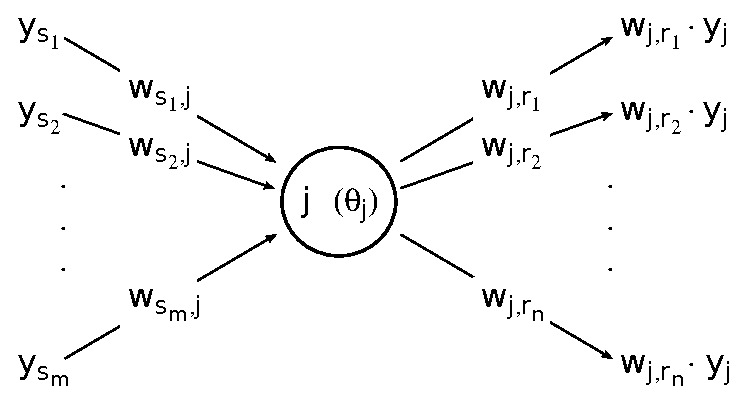
\includegraphics[scale = 0.55]{neural_model.eps}
			\end{minipage}
			\begin{minipage}{0.49\textwidth}
				\center
				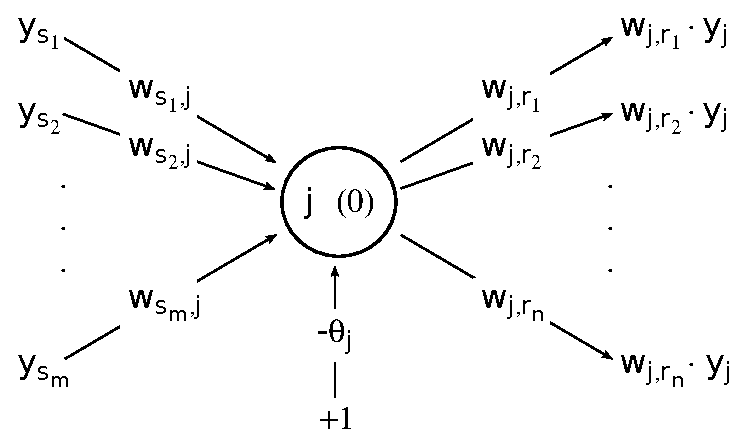
\includegraphics[scale = 0.55]{neural_model_bias.eps}
			\end{minipage}
		
			\caption{Visualization of the generic $j$-th neuron of an artificial neural network, including (right) or not (left) a bias neuron. On the left, the neuron accumulates the weighted inputs $\big\lbrace w_{s_1,j} ~ y_{s_1}, \, \ldots \, , w_{s_m,j} ~ y_{s_m} \big\rbrace$ respectively coming from the sending neurons $\big\lbrace s_1, \, \ldots \, , s_m \big\rbrace$; on the right, the neuron accumulates the weighted inputs $\big\lbrace w_{s_1,j} ~ y_{s_1}, \, \ldots \, , w_{s_m,j} ~ y_{s_m}, \, -\theta_j \big\rbrace$ respectively coming from the sending neurons $\big\lbrace s_1, \, \ldots \, , s_m, \, b \big\rbrace$, with $b$ the bias neuron. In both situations, the neuron then fires $y_j$, sent to the target neurons $\big\lbrace r_1, \, \ldots \, , r_n \big\rbrace$ through the synapsis $\big\lbrace w_{j,r_1}, \, \ldots \, , w_{j,r_n} \big\rbrace$. The neuron threshold is reported in brackets within its body.} 
			\label{fig:neural-model}
		\end{figure}
		
		
	%
	% Subsection 4.2 : Network topology
	%
	
	\subsection{Network topology: the feedforward neural network}
	\label{section:Network topology}
	
		The interconnection of neurons within a network defines the \emph{topology} of the network itself, i.e., its design. In the literature, many network architectures have been proposed, sometimes tailored to a specific application. Among all, \emph{feedforward neural networks}, also called \emph{perceptrons} \cite{Ros58}, have been preferred in function regression tasks.
		
		In a feedforward neural network, neurons are arranged into \emph{layers}, with one \emph{input layer} of $M_I$ source neurons, $K$ \emph{hidden layers}, each one consisting of $H_k$ computing neurons, $k = 1, \, \ldots \, , K$, and an \emph{output layer} of $M_O$ computing neurons. As a characteristic property, neurons in a layer can only be connected with neurons in the next layer towards the output layer. When an \textcolor{red}{input vector} $\mathbf{p} \in \mathbb{R}^{M_I}$ is supplied to the network through the source nodes, this provides the input signal for the neurons in the first hidden layer. \textcolor{red}{In turn, the outputs of each hidden layer feed the neurons in the following layer}. In this way, information travels towards the output layer, whose outputs constitute the components of the overall output $\mathbf{q} \in \mathbb{R}^{M_O}$ of the network \footnote{Please note that while the output of a single neuron is denoted with the letter $y$, we use the letter $\mathbf{q}$ (bolded) to indicate the overall output of the network. Clearly, for the $j$-th output neuron, its output $y_j$ coincides with the corresponding entry of $\mathbf{q}$, i.e., $q_j = y_j$ for any $j = 1, \, \ldots \, , M_O$.}. Hence, a feedforward network establishes a map between the \emph{input space} $\mathbb{R}^{M_I}$ and the \emph{output space} $\mathbb{R}^{M_O}$. This does make this network architecture particularly suitable for continuous function approximation.
		
		Feedforward networks can be classified according to the number of hidden layers or, equivalently, the number of layers of trainable weights. Single-layer perceptrons (SLPs) consist of the input and output layer, without any hidden layer. Because of their simple structure, the range of application of SLPs is rather limited. Indeed, only \emph{linearly separable} data can be properly represented using SLPs \cite{Kri07}. Conversely, multi-layer perceptrons (MLPs), with at least one hidden layer, are universal function approximators, as stated by Cybenko \cite{Cyb88, Cyb89}. In detail:
		\begin{enumerate}[label=(\roman*)]
			\item MLPs with \emph{one} hidden layer and differentiable activation functions can approximate \emph{any continuous} function; 
			\label{cybenko-first-rule}
			\item MLPs with \emph{two} hidden layers and differentiable activation functions can approximate \emph{any} function. 		
			\label{cybenko-second-rule}
		\end{enumerate}
		Therefore, in many practical applications there is no reason to employ MLPs with more than two hidden layers. However, \ref{cybenko-first-rule} and \ref{cybenko-second-rule} do not give any practical advice neither on the number of hidden neurons nor the number of samples required to train the network: these should be found pursuing a \emph{trial-and-error} (and likely time-consuming) approach \cite{Hag96}.
		
		An instance of a three-layer (i.e., two hidden layer plus the output layer) feedforward network is offered in Fig. \ref{fig:neural-network}. In this case, we have $M_I = 3$ input neurons (denoted with the letter $i$), $H_1 = H_2 = 6$ hidden neurons (letter $h$ for both hidden layers), and $M_O = 4$ output neurons (letter $o$). In particular, it represents an instance of a \emph{completely linked} perceptron, since each neuron is directly connected with all neurons in the following layer.
				
		\begin{figure}[t]
			\center
			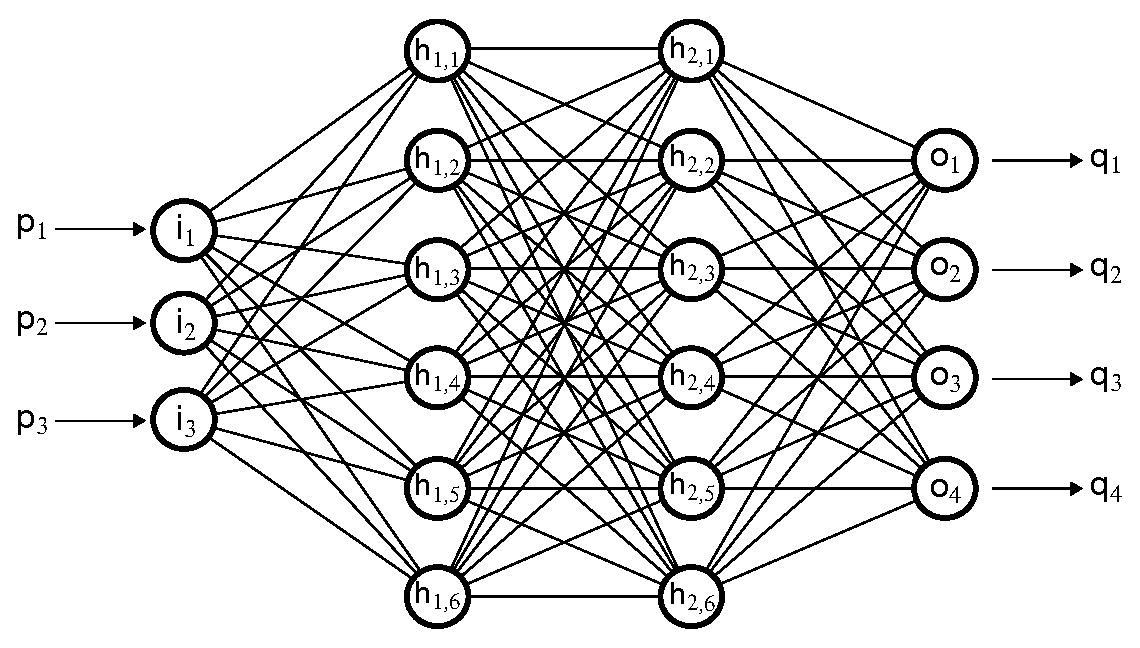
\includegraphics[scale = 0.55]{neural_network.eps}
			
			\caption{A three-layer feedforward neural network, with three input neurons, two hidden layers each one consisting of six neurons, and four output neurons. Within each connection, information flows from left to right.}
			\label{fig:neural-network}
		\end{figure}
		
		
	%
	% Subsection 4.3 : Training a multi-layer feedforward neural network
	%
	
	\subsection{Training a multi-layer feedforward neural network}
	\label{section:Training a multi-layer feedforward neural network}
	
		As previously mentioned, the principal characteristic of a neural network is its capability of \emph{learning} from the surrounding environment, storing the acquired knowledge via its internal parameters, i.e., the synaptic and bias weights. Learning is accomplished through a training process, during which the network is exposed to a collection of examples, called \textcolor{red}{\emph{training data}}. According to some performance measure, the weights are then adjusted by means of a well-defined set of rules. Therefore, the learning procedure is an \emph{algorithm}, typically iterative, such that after a successfull training, the neural network provides reasonable responses for unknown problems of the same class of the training set. This property is known as \emph{generalization} \cite{Kri07}. 
		
		Training algorithms can be classified based on the nature of the training set, i.e., the set of \textcolor{red}{training data}. We can then distinguish three \emph{learning paradigms}: supervised learning, unsupervised learning and reinforcement learning \cite{Hag96}. The choice of the learning paradigm is clearly task-dependent. Particularly, for function approximation, the \emph{supervised} learning paradigm is the natural choice. 
		
		Consider the nonlinear unknown function $\bg{f} ~ : ~ \mathbb{R}^{M_I} \rightarrow \mathbb{R}^{M_O}$ and a set of labeled examples \smash{$\big\lbrace \mathbf{p}_i, \mathbf{t}_i = \bg{f}(\mathbf{p}_i)\big\rbrace_{1 \leq i \leq N_{tr}}$}, which form the training set. Note that to each \textcolor{red}{\emph{training input}} $\mathbf{p}_i \in \mathbb{R}^{M_I}$, $i = 1, \, \ldots \, , N_{tr}$, corresponds an associated \textcolor{red}{\emph{desired output}} $\mathbf{t}_i \in \mathbb{R}^{M_O}$. The goal is to approximate $\bg{f}$ over a domain $D \subset \mathbb{R}^{M_I}$ up to a user-defined tolerance $\epsilon$, i.e.,
		\begin{linenomath}\begin{equation*}
			||\bg{F}(\mathbf{x}) - \boldsymbol{f}(\mathbf{x})|| < \epsilon \hspace*{0.3cm} \text{$\forall \mathbf{x} \in D$} \, ,
		\end{equation*}\end{linenomath}
		where $\bg{F} : \mathbb{R}^{M_I} \rightarrow \mathbb{R}^{M_O}$ is the actual input-output map established by the neural network and $||\cdot||$ is some suitable norm on $\mathbb{R}^{M_O}$. For this purpose, consider the synapsis between a sending neuron $i$ and a target neuron $j$. At the $t$-th iteration (also called \emph{epoch}) of the training procedure, the weight $w_{i,j}(t)$ of the connection $(i,j)$ is modified by the time-dependent quantity $\Delta w_{i,j}(t)$, whose form depends on the specific learning rule. Hence, at the subsequent iteration $t+1$ the synaptic weight is simply given by
		\begin{linenomath}\begin{equation*}
			w_{i,j}(t+1) = w_{i,j}(t) + \Delta w_{i,j}(t) \, .
		\end{equation*}\end{linenomath}
		The whole training process is driven by an \emph{error} or \emph{performance} function $E$, which measures the discrepancy between the neural network knowledge of the surrounding environment and the actual state of the environment itself. Therefore, every learning rule aims to \emph{minimize} the performance $E$, thought as a scalar function of the free parameters of the network, namely 
		\begin{linenomath}\begin{equation*}
			E = E(\mathbf{w}) \in \mathbb{R} \, , 
		\end{equation*}\end{linenomath}
		with $\mathbf{w} \in \mathbb{R}^{W}$ being the vector collecting all the synaptic and bias weights. Thus, the point over the error surface reached at the end of a successful training process provides the \emph{optimal} configuration $\mathbf{w}_{opt}$ for the network. A common choice for the performance function is the (accumulated) mean squared error (MSE)
		\begin{linenomath}\begin{linenomath}\begin{equation}
			\label{eq:accumulated-mse}
			E(\mathbf{w}) = \sum_{\mathbf{p} \in P} E_{\mathbf{p}}(\mathbf{w}) = \sum_{\mathbf{p} \in P} \dfrac{1}{M_O} \sum_{j = 1}^{M_O} \left( t_{\mathbf{p},j} - q_{\mathbf{p},j} \right)^2 \, ,
		\end{equation}\end{linenomath}\end{linenomath}
		where for each \textcolor{red}{input vector} $\mathbf{p}$ belonging to the training set $P$, $\mathbf{t}_{\mathbf{p}}$ and $\mathbf{q}_{\mathbf{p}}$ denote respectively the corresponding \textcolor{red}{desired} and actual output. Observe that \eqref{eq:accumulated-mse} accounts for the error committed on each \textcolor{red}{input vector} in the training set, leading to an \emph{offline} learning procedure.
		
		In our numerical tests, the weights are iteratively adjusted via the Levenberg-Marquardt (\textcolor{deepgreen}{LM}) algorithm \cite{Lev44, Mar63}. \textcolor{red}{With respect to the notation used in \cite{Hag94}, in our numerical tests we set $\mu = 0.001$ as starting point for the bias parameter $\mu$, with the damping factor $\beta$ equal to $10$}. As pointed out in \cite{Hag96}, the cost of the \textcolor{deepgreen}{LM} algorithm increases nonlinearly with the number of neurons in the network, making it poorly efficient for large networks. However, it turns out to be efficient and accurate for networks with few hundreads of connections.  		

	%
	% Section 5 : POD-NN method
	%
	
	\section{A non-intrusive reduced basis method using artificial neural networks}
	\label{section:A non-intrusive RB method using neural networks}
							
		The scenario portrayed so far motivates the research for an alternative approach to tackle any online query within the reduced basis framework. To this end, let us remark that there exists a one-to-one correspondence between the reduced space $V_{\texttt{rb}}$ and the column space $\text{Col}(\mathbb{V})$ of $\mathbb{V}$. Indeed, letting $\big\lbrace \phi_1, \, \ldots \, , \phi_{N_h} \big\rbrace$ be a basis for $V_h$ and $\big\lbrace \psi_1, \, \ldots \, , \psi_L \big\rbrace$ be the reduced basis, from Eq. \eqref{eq:change-of-variables} follows:
		\begin{linenomath}\begin{equation*}
			V_{\texttt{rb}} \ni v_{L} = \sum_{j = 1}^L v_{\texttt{rb}}^{(j)} ~ \psi_j = \sum_{j = 1}^L v_{\texttt{rb}}^{(j)} \sum_{i = 1}^{N_h} \mathbb{V}_{i,j} ~ \phi_i = \sum_{i = 1}^{N_h} \big( \mathbb{V} ~ \mathbf{v}_{\texttt{rb}} \big)_i \phi_i \hspace*{0.3cm} \leftrightarrow \hspace*{0.3cm} \mathbf{v}_L^{} \in \text{Col}(\mathbb{V}) \, .
		\end{equation*}\end{linenomath} 
		In particular, this implies that the projection of any $v_h \in V_h$ onto $V_{\texttt{rb}}$ in the discrete scalar product $(\cdot,\cdot)_h$, 
		\begin{linenomath}\begin{linenomath}\begin{equation}
			\label{eq:discrete-scalar-product}
			(\chi_h, \, \xi_h)_h = \sum_{i = 1}^{N_h} \chi_h^{(i)} ~ \xi_h^{(i)} = (\bg{\chi}_h, \, \bg{\xi}_h)_{\mathbb{R}^{N_h}} \hspace*{0.3cm} \text{$\forall \chi_h, \, \xi_h \in V_h$} \, , 
		\end{equation}\end{linenomath}\end{linenomath}
		algebraically corresponds to the projection $\mathbf{v}_h^{\mathbb{V}}$ of $\mathbf{v}_h$ onto $\text{Col}(\mathbb{V})$ in the Euclidean scalar product, given by
		\begin{linenomath}\begin{equation*}
			\mathbf{v}_h^{\mathbb{V}} = \mathbb{P} ~ \mathbf{v}_h \hspace*{0.5cm} \text{with} \hspace*{0.5cm} \mathbb{P} = \mathbb{V} \mathbb{V}^T \in \mathbb{R}^{{N_h} \times {N_h}} \, .
		\end{equation*}\end{linenomath}
		Note that $\mathbf{v}_h^{\mathbb{V}}$ is the element of $\text{Col}(\mathbb{V})$ closest to $\mathbf{v}_h$ in the Euclidean norm, i.e.,
		\begin{linenomath}\begin{equation*}
			\norm{\mathbf{v}_h - \mathbf{v}_h^{\mathbb{V}}}_{\mathbb{R}^{N_h}} = \inf_{\mathbf{w}_h \in \text{Col}(\mathbb{V})} \norm{\mathbf{v}_h - \mathbf{w}_h}_{\mathbb{R}^{N_h}} \, .
		\end{equation*}\end{linenomath}
		Therefore, the element of $V_{\texttt{rb}}$ closest to the high-fidelity solution $u_h$ in the discrete norm $\norm{\cdot}_h = \sqrt{(\cdot,\cdot)_h}$ can be expressed as
		\begin{linenomath}\begin{equation*}
			\label{eq:high-fidelity-projected}
			u^{\mathbb{V}}_h(\bg{x}; \, \bg{\mu}) = \sum_{j = 1}^{N_h} \big( \mathbb{V} \mathbb{V}^T \mathbf{u}_h(\bg{\mu}) \big)_j \phi_j(\bg{x}) = \sum_{i = 1}^L \big( \mathbb{V}^T \mathbf{u}_h(\bg{\mu}) \big)_i ~ \psi_i(\bg{x}) \, .
		\end{equation*}\end{linenomath} 
		Motivated by this last equality, once a reduced basis has been constructed (e.g., via POD of the snapshot matrix), we aim at approximating the function
		\begin{linenomath}\begin{linenomath}\begin{equation}
			\label{eq:map-to-approximate}
			\begin{aligned}
				\bg{\pi} ~ : ~ \mathcal{P} \subset \mathbb{R}^P ~ & \rightarrow ~ \mathbb{R}^L \\
				\bg{\mu} ~~ & \mapsto ~ \mathbb{V}^T \mathbf{u}_h(\bg{\mu}) \, ,
			\end{aligned}
		\end{equation}\end{linenomath}\end{linenomath}
		which maps each input vector parameter $\bg{\mu} \in \mathcal{P}$ to the coefficients $\mathbb{V}^T \mathbf{u}_h(\bg{\mu})$ for the expansion of $u^{\mathbb{V}}_h$ in the reduced basis $\big\lbrace \psi_i \big\rbrace_{1 \leq i \leq L}$. Then, given a new parameter instance $\bg{\mu}$, the associated RB solution is simply given by the evaluation at $\bg{\mu}$ of the so-built approximation $\hat{\bg{\pi}}$ of $\bg{\pi}$, i.e.
		\begin{linenomath}\begin{equation*}
			\mathbf{u}_{\texttt{rb}}(\bg{\mu}) = \hat{\bg{\pi}}(\bg{\mu}) \, ,
		\end{equation*}\end{linenomath}
		and, consequently,
		\begin{linenomath}\begin{equation*}
			\mathbf{u}_L(\bg{\mu}) = \mathbb{V} ~ \hat{\bg{\pi}}(\bg{\mu}) \, .
		\end{equation*}\end{linenomath}
		Note that, provided that the construction of $\hat{\bg{\pi}}$ is carried out within the offline stage, this approach leads to a \emph{non-intrusive} RB method, enabling a complete decoupling between the online step and the underlying full-order model. Moreover, the accuracy of the resulting reduced solution uniquely relies on the quality of the reduced basis and the effectiveness of the approximation $\hat{\bg{\pi}}$ of the map $\bg{\pi}$, which we assume sufficiently smooth. 

		In the literature, different approaches for the \emph{interpolation} of \eqref{eq:map-to-approximate} have been developed, e.g., exploiting some geometrical considerations concerning the discrete solution manifold $\mathcal{M}_h$ \cite{Ams10}, or employing radial basis functions \cite{Chen17}. In this work we resort to artificial neural networks for the \emph{nonlinear regression} of the map $\bg{\pi}$, leading to the POD-NN RB method. As described in Subsection \ref{section:Training a multi-layer feedforward neural network}, any neural network is tailored to the particular application at hand by means of a preliminary \emph{training} phase. Here, we are concerned with a function regression task, thus we straightforwardly adopt a \emph{supervised learning} paradigm, training the perceptron via exposition to a collection of (known) input-output pairs
		\begin{linenomath}\begin{equation*}
			P_{tr} = \big\lbrace \big( ~ \bg{\mu}^{(i)}, \, \mathbb{V}^T \mathbf{u}_h \big( \bg{\mu}^{(i)} \big) ~ \big) \big\rbrace_{1 \leq i \leq N_{tr}} \, .
		\end{equation*}\end{linenomath} 
		According to the notation and nomenclature previously introduced, for any $i = 1, \, \ldots \, , N_{tr}$, $\mathbf{p}_i = \bg{\mu}^{(i)} \in \mathbb{R}^P$ represents the \textcolor{red}{\emph{training input}} and $\mathbf{t}_i =  \mathbb{V}^T \mathbf{u}_h \big( \bg{\mu}^{(i)} \big) \in \mathbb{R}^L$ the associated \textcolor{red}{\emph{desired output}}. In this respect, note that the \textcolor{red}{output vectors} $\mathbb{V}^T \mathbf{u}_h \big( \bg{\mu}^{(i)} \big)$, $i = 1, \, \ldots \, , N_{tr}$, are generated through the FE solver. On the one hand, this ensures the reliability of the \textcolor{red}{teaching data}, given the assumed high-fidelity of the FE scheme.	On the other hand, this also suggests to incorporate the learning phase of the perceptron in the offline step of the POD-NN RB method, as described in Algorithm \ref{alg:pod-nn}. In doing so, we exploit the natural decoupling between the training and the evaluation of neural networks, thus fulfilling the necessary requirement to ensure online efficiency. 						

		\algrenewcommand\textproc{}
		
		\begin{algorithm}[t!]	
			\begin{algorithmic}[1]
				\Function{$\big[ \mathbb{V}, \mathbf{w}_{\texttt{rb}} \big] = $ \textsc{PODNN\_offline}}{$\mathcal{P}$, $\Omega_h$, $N$}
					\State generate the parameter set $\Xi_N = \big\lbrace \bg{\mu}^{(1)}, \, \ldots \, , \bg{\mu}^{(N)} \big\rbrace$
					\State compute the high-fidelity solutions $\big\lbrace \mathbf{u}_h \big( \bg{\mu}^{(1)} \big), \, \ldots \, , \mathbf{u}_h \big( \bg{\mu}^{(N)} \big) \big\rbrace$ via FE-Newton's method
					\State generate the POD basis functions $\big\lbrace \mathbf{w}_1, \, \ldots \, , \mathbf{w}_L \big\rbrace$ via method of snapshots
					\State assemble $\mathbb{V} = \big[ \mathbf{w}_1 \, \big| \, \ldots \, \big| \, \mathbf{w}_L \big]$
					\State find an optimal network configuration $\mathbf{w}_{\texttt{rb}}$ relying upon LHS and Levenberg-Marquardt algorithm
				\EndFunction
				
				\vspace*{0.3cm}
				
				\setcounter{ALG@line}{0}
				
				\Function{$\mathbf{u}_L^{\texttt{NN}} (\bg{\mu}) = $ \textsc{PODNN\_online}}{$\bg{\mu}$, $\mathbb{V}$, $\mathbf{w}_{\texttt{rb}}$}
					\State evaluate the output $\mathbf{u}_{\texttt{rb}}^{\texttt{NN}}(\bg{\mu})$ of the network for the input vector $\bg{\mu}$
					\State compute $\mathbf{u}_L^{\texttt{NN}} (\bg{\mu}) = \mathbb{V} \, \mathbf{u}_{\texttt{rb}}^{\texttt{NN}}(\bg{\mu})$
				\EndFunction
			\end{algorithmic}
			
			\caption{The offline and online stages for the POD-NN RB method.}
			\label{alg:pod-nn}
		\end{algorithm}
		
		It should be pointed out that the design of an effective learning procedure may require a larger amount of snapshots than the generation of the reduced space does. Moreover, we mentioned in Subsection \ref{section:Network topology} the time-consuming yet unavoidable \emph{trial}-\emph{and}-\emph{error} approach which one should pursue in the search for an optimal network topology. To this end, we propose an automatic procedure.

		While Cybenko's theorems (see Subsection \ref{section:Network topology}) allow one to consider perceptrons with no more than two hidden layers, no similar a priori and general results are available for the number $H$ of neurons per layer \footnote{ Here we uniquely consider networks with the same number of neurons in both the first and the second hidden layer, but this is not required.}. Hence, given an initial amount $N_{tr}$ of training samples (say $N_{tr} = 100$), we train the network for increasing values of $H$, stopping when overfitting of training data occurs, due to an excessive number of neurons. In case the best configuration, i.e., the one yielding the smallest error on a \emph{test} data set, does not meet a desired level of accuracy, we generate a new set of snapshots, which will enlarge the current training set, and then proceed to re-train the network in different configurations. At this point, it is worth pointing out two issues. 
		\begin{enumerate}[label=(\roman*)]
			\vspace*{-0.1cm}
			\item Once the training set has been enriched, we can limit ourselves to network configurations including a number of neurons \emph{no smaller} than the current optimal network. Indeed, the error on the test data set is decreasing in the number of \textcolor{red}{training data} the neural network is exposed to during the learning phase, and the larger the number of neurons, the faster the decay.
			\item In order to maximize the additional quantity of information available for the learning, we should ensure that the new training inputs, i.e., parameter values, do not overlap with the ones already present in the training parameter set. To this aim, we pursue an heuristhic approach, employing, at each iteration, the latin hypercube sampling \cite{Imam08}, which provides a good compromise between randomness and even coverage of the parameter domain. 	
		\end{enumerate} 
		\vspace*{-0.1cm}
		The procedure is then iterated until a satisfactory degree of accuracy and generalization is attained, or the available resources (i.e., computing power, running time and memory space) are exhausted. Therefore, the speed-up enabled at the \emph{online} stage comes at the cost of an extended \emph{offline} phase. 
		
		In our numerical tests, we rely on the mean squared error \eqref{eq:accumulated-mse} as performance function driving the neural network training process. To motivate this choice, let 
		\begin{linenomath}\begin{equation*}
			\mathbf{u}_{\texttt{rb}}^{\texttt{NN}}(\bg{\mu}) \in \mathbb{R}^L
		\end{equation*}\end{linenomath}
		be the (actual) output provided by the network for a given input $\bg{\mu}$, and 
		\begin{linenomath}\begin{equation*}
			\mathbf{u}_L^{\texttt{NN}}(\bg{\mu}) = \mathbb{V} ~ \mathbf{u}_{\texttt{rb}}^{\texttt{NN}}(\bg{\mu}) \in \text{Col}(\mathbb{V}) \subset \mathbb{R}^{N_h} \, . 
		\end{equation*}\end{linenomath}
		Then (omitting the dependence on the input vector for ease of notation):
		\begin{linenomath}\begin{equation*}
				MSE \big( \mathbf{u}_{\texttt{rb}}^{\texttt{NN}}, \, \mathbb{V}^T \mathbf{u}_h \big) \propto \norm{\mathbf{u}_{\texttt{rb}}^{\texttt{NN}} - \mathbb{V}^T \mathbf{u}_h}^2_{\mathbb{R}^L} = \norm{\mathbf{u}_L^{\texttt{NN}} - \mathbb{V} ~ \mathbb{V}^T \mathbf{u}_h}^2_{\mathbb{R}^{N_h}} = \norm{u_L^{\texttt{NN}} - u_h^{\mathbb{V}}}^2_h \, ,
		\end{equation*}\end{linenomath} 
		where
		\begin{linenomath}\begin{equation*}
			\label{eq:pod-nn-solution}
			u_L^{\texttt{NN}}(\bg{x}; \, \bg{\mu}) = \sum_{i = 1}^L \big( \mathbf{u}_{\texttt{rb}}^{\texttt{NN}}(\bg{\mu}) \big)_i ~ \psi_i(\bg{x}) ~ \in ~ V_{\texttt{rb}} \, .
		\end{equation*}\end{linenomath}
		Therefore, for any training input $\bg{\mu}^{(i)}$, $i = 1, \, \ldots \, , N_{tr}$, by minimizing the MSE we minimize the distance (in the discrete norm $\norm{\cdot}_h$) between the approximation provided by the neural network and the projection of the FE solution onto the reduced space $V_{\texttt{rb}}$. The proper \emph{generalization} to other parameter instances, not included in the training set, is then ensured by the implementation of suitable techniques (e.g., early stopping \cite{Mat16}, generalized cross validation \cite{Koh95}) aiming at preventing the network to \emph{overfit} the training data.
		
			
	%
	% Section 6 : Numerical results
	%
	
	\section{Numerical results}
	\label{section:Numerical results}
	
		In this section, we present the numerical results obtained via the FE, POD-G and POD-NN methods applied to parametrized full-Dirichlet boundary value problems (BVPs) for the one-dimensional and two-dimensional nonlinear Poisson equation and the two-dimensional incompressible steady Navier-Stokes equations. In the one-dimensional case we deal uniquely with physical parameters, whereas in two spatial dimensions we consider purely geometric parametrizations. 	

		The two RB techniques considered in this work are compared both in terms of accuracy and performance during the online stage. For this, let $\norm{\cdot}$ be the canonical (Euclidean) norm on $\mathbb{R}^{N_h}$. In the online phases of the POD-G and POD-NN methods, for a new parameter value $\bg{\mu} \in \mathcal{P}$ (not involved either in the generation of the POD basis nor in the identification of an optimal neural network), the following \emph{relative} errors with respect to the high-fidelity solution $\mathbf{u}_h(\bg{\mu})$ are analyzed:
		\begin{enumerate}[label=(\alph*)]
			\item the POD-G relative error,
			\begin{linenomath}\begin{linenomath}\begin{equation}
				\label{eq:podg-error}
				\varepsilon_{\texttt{PODG}}^{}(L, \bg{\mu}) = \dfrac{\norm{\mathbf{u}_h(\bg{\mu}) - \mathbf{u}_L(\bg{\mu})}}{\norm{\mathbf{u}_h(\bg{\mu})}} = \dfrac{\norm{\mathbf{u}_h(\bg{\mu}) - \mathbb{V} \, \mathbf{u}_{\texttt{rb}}(\bg{\mu})}}{\norm{\mathbf{u}_h(\bg{\mu})}} \, ;
			\end{equation}\end{linenomath}\end{linenomath} 
			\item the POD-NN relative error,
			\begin{linenomath}\begin{linenomath}\begin{equation}
				\label{eq:podnn-error}
				\varepsilon_{\texttt{PODNN}}^{}(L, \bg{\mu}) = \dfrac{\norm{\mathbf{u}_h(\bg{\mu}) - \mathbf{u}_L^{\texttt{NN}}(\bg{\mu})}}{\norm{\mathbf{u}_h(\bg{\mu})}} = \dfrac{\norm{\mathbf{u}_h(\bg{\mu}) - \mathbb{V} \, \mathbf{u}_{\texttt{rb}}^{\texttt{NN}}(\bg{\mu})}}{\norm{\mathbf{u}_h(\bg{\mu})}} \, ;
			\end{equation}\end{linenomath}\end{linenomath} 
			\item the relative projection error, i.e., the error committed by approximating the high-fidelity solution with its projection (in the discrete scalar product $(\cdot,\cdot)_h$, see \eqref{eq:discrete-scalar-product}) onto the reduced space $V_{\texttt{rb}}$,
			\begin{linenomath}\begin{linenomath}\begin{equation}
				\label{eq:projection-error}
				\varepsilon_{\mathbb{V}}^{}(L, \bg{\mu}) = \dfrac{\norm{\mathbf{u}_h(\bg{\mu}) - \mathbf{u}_h^{\mathbb{V}}(\bg{\mu})}}{\norm{\mathbf{u}_h(\bg{\mu})}} = \dfrac{\norm{\mathbf{u}_h(\bg{\mu}) - \mathbb{V} \mathbb{V}^T \mathbf{u}_h(\bg{\mu})}}{\norm{\mathbf{u}_h(\bg{\mu})}} \, .
			\end{equation}\end{linenomath}\end{linenomath}
			Clearly, \eqref{eq:projection-error} provides a lower-bound for both \eqref{eq:podg-error} and \eqref{eq:podnn-error}.  
		\end{enumerate}
		The above errors are evaluated on a \emph{test} parameter set $\Xi_{te} \subset \mathcal{P}$ consisting of $N_{te}$ randomly picked samples. Given that a sufficiently large number of test values is chosen, statistics for $\varepsilon_{\texttt{PODG}}^{}(L, \cdot)$, $\varepsilon_{\texttt{PODNN}}^{}(L, \cdot)$ and $\varepsilon_{\mathbb{V}}^{}(L, \cdot)$ on $\Xi_{te}$ can be reasonably assumed independent of the particular choice made for $\Xi_{te}$, thus making any subsequent error analysis reliable. In particular, in our numerical studies we let $N_{te}$ range from $50$ up to $100$, and we consider the average of the errors over the test data set, respectively denoted by
		\begin{linenomath}\begin{equation*}
			\bar{\varepsilon}_{\texttt{PODG}}^{} = \bar{\varepsilon}_{\texttt{PODG}}^{}(L) = \dfrac{\sum_{\bg{\mu} \in \Xi_{te}} \varepsilon_{\texttt{PODG}}^{}(L, \bg{\mu})}{N_{te}} \, , \qquad \bar{\varepsilon}_{\texttt{PODNN}}^{} = \bar{\varepsilon}_{\texttt{PODNN}}^{}(L) = \dfrac{\sum_{\bg{\mu} \in \Xi_{te}} \varepsilon_{\texttt{PODNN}}^{}(L, \bg{\mu})}{N_{te}} \, , \qquad \bar{\varepsilon}_{\mathbb{V}}^{} = \bar{\varepsilon}_{\mathbb{V}}^{}(L) = \dfrac{\sum_{\bg{\mu} \in \Xi_{te}} \varepsilon_{\mathbb{V}}^{}(L, \bg{\mu})}{N_{te}} \, .
		\end{equation*}\end{linenomath}
		In the training phase of neural networks, we rely upon the well-known cross-validation procedure \cite{Koh95}. While the training samples $\Xi_{tr} \subset \mathcal{P}$ are generated via successive latin hypercube samplings (as explained in Section \ref{section:A non-intrusive RB method using neural networks}), the \emph{validation} inputs $\Xi_{va} \subset \mathcal{P}$ are randomly picked through a Monte Carlo sampling, as done for $\Xi_{te}$. The ratio between the size of $\Xi_{va}$ and $\Xi_{tr}$ is set to $0.3$. \textcolor{red}{At the beginning of the learning process, the weights are randomly initialized using a standard Gaussian distribution. To limit the dependence of the results on the starting configuration, we pursue the \emph{multiple restarts} approach; see, e.g., \cite{Kri07, Mat16}.} Typically, five restarts are performed per network topology. \textcolor{red}{Within each restart, an early stopping technique is implemented to further prevent overfitting: training is immediately stopped when the validation error increases over $K_{ea}$ consecutive epochs \cite{Mat16}. Here, $K_{ea} = 6$ is used.} To ease the research for an optimal network configuration and by exploiting Cybenko's results (see Subsection \ref{section:Network topology}), we limit ourselves to three-layers neural networks, with the same number of neurons for both hidden layers. For each topology, the hyperbolic tangent is used as activation function for the hidden neurons. 		
		All the results presented in the following subsections have been obtained via a MATLAB\textsuperscript{\textregistered} implementation of the FE, POD-G and POD-NN methods, with all the simulations carried out on a laptop equipped with a CPU Intel\textsuperscript{\textregistered} Core\textsuperscript{TM} i7 @ 2.50 GHz.
				
		
	%
	% Subsection 6.1 : Nonlinear Poisson equation
	%
	
	\subsection{Nonlinear Poisson equation}
	\label{section:Nonlinear Poisson equation}
		
		Despite a rather simple form, the Poisson equation has proved itself to be effective to model steady phenomena occurring in, e.g., electromagnetism, heat transfer and underground flows \cite{MM10}. We consider the following version of the parametrized Poisson equation for a state variable $\wt{u} = \wt{u}(\bg{\mu})$:		
		\begin{subequations}
			\label{eq:poisson-differential}
			\begin{empheq}[left=\empheqlbrace]{align}
				\label{eq:poisson-differential-first-equation}
				- \wt{\nabla} \cdot \left( \wt{k}(\wt{\bg{x}}, \, \wt{u}(\bg{\mu}); \bg{\mu}_{ph}) ~ \wt{\nabla} \wt{u}(\bg{\mu}) \right) & = \wt{s}(\wt{\bg{x}}; \, \bg{\mu}_{ph}) & \hspace*{-2cm} \text{in $\wt{\Omega}(\bg{\mu}_g)$} \, , \\
				\wt{u}(\bg{\mu}) & = \wt{h}(\wt{\bg{\sigma}}; \, \bg{\mu}_{ph}) & \hspace*{-2cm} \text{on $\wt{\Gamma}_D$} \, , \\
				\wt{k}(\wt{\bg{\sigma}}, \, \wt{u}(\bg{\mu}); \bg{\mu}_{ph}) ~ \wt{\nabla} \wt{u}(\bg{\mu}) \cdot \wt{\bg{n}} & = 0 & \hspace*{-2cm} \text{on $\wt{\Gamma}_N$} \, .
			\end{empheq}
		\end{subequations}
		Here, for any $\bg{\mu}_g \in \mathcal{P}_g$, $\wt{\bg{x}}$ and $\wt{\bg{\sigma}}$ denote a generic point in $\wt{\Omega}$ and on $\wt{\Gamma}$, respectively, $\wt{\nabla}$ is the nabla operator with respect to $\wt{\bg{x}}$, $\wt{\bg{n}} = \wt{\bg{n}}(\wt{\bg{\sigma}})$ denotes the outward normal to $\wt{\Gamma}$ in $\wt{\bg{\sigma}}$, $\wt{k} ~ : ~ \wt{\Omega} \times \mathbb{R} \times \mathcal{P}_{ph} \rightarrow (0,\infty)$ is the diffusion coefficient, $\wt{s} ~ : ~ \wt{\Omega} \times \mathcal{P}_{ph} \rightarrow \mathbb{R}$ is the source term, and $\wt{h} ~ : ~ \wt{\Gamma}_D \times \mathcal{P}_{ph} \rightarrow \mathbb{R}$ encodes the Dirichlet boundary conditions. To ease the subsequent discussion, we limit the attention to homogeneous Neumann boundary constraints.
		
		Let us fix $\bg{\mu} \in \mathcal{P}$ and set 
		\begin{linenomath}\begin{equation*}
			\wt{V} = \wt{V}(\bg{\mu}_g) = H^1_{\wt{\Gamma}_D} \big( \wt{\Omega}(\bg{\mu}_g) \big) = \big\lbrace v \in H^1 \big( \wt{\Omega}(\bg{\mu}_g) \big) ~ : ~ v \big\rvert_{\wt{\Gamma}_D} = 0 \big\rbrace \, ,
		\end{equation*}\end{linenomath}
		Multiplying \eqref{eq:poisson-differential-first-equation} by a \emph{test} function $v \in \wt{V}$, integrating over $\wt{\Omega}$, and exploiting integration by parts on the left-hand side, yields:
		\begin{linenomath}\begin{linenomath}\begin{equation}
			\label{eq:poisson-weak-derivation}
			\int_{\wt{\Omega}(\bg{\mu}_g)} \wt{k}(\wt{u}(\bg{\mu}); \, \bg{\mu}_{ph}) ~ \wt{\nabla} \wt{u}(\bg{\mu}) \cdot \wt{\nabla} v ~ d\wt{\Omega}(\bg{\mu}_g) = \int_{\wt{\Omega}(\bg{\mu}_g)} \wt{s}(\bg{\mu}_{ph}) ~ v ~ d\wt{\Omega}(\bg{\mu}_g) \, ,
		\end{equation}\end{linenomath}\end{linenomath}
		where we have omitted the dependence on the space variable $\wt{\bg{x}}$ for ease of notation. For the integrals in Eq. \eqref{eq:poisson-weak-derivation} to be well-defined, we require, for any $\bg{\mu}_g \in \mathcal{P}_g$, 
		\begin{linenomath}\begin{equation*}
			\text{$|\wt{k}(\wt{\bg{x}}, \, r; \, \bg{\mu}_g)| < \infty$ for almost any (a.a.) $\wt{\bg{x}} \in \wt{\Omega}(\bg{\mu}_g), \, r \in \mathbb{R}$} \, , ~~ \text{and} ~~ \wt{s}(\bg{\mu}_{ph}) \in L^2 \big( \wt{\Omega}(\bg{\mu}_g) \big) \, .
		\end{equation*}\end{linenomath}
		Let then $\wt{l} = \wt{l}(\bg{\mu}) \in H^1 \big( \wt{\Omega}(\bg{\mu}_g) \big)$ be a \emph{lifting} function such that $\wt{l}(\bg{\mu}) \big\rvert_{\wt{\Gamma}_D} = \wt{h}(\bg{\mu}_{ph})$, with $\wt{h}(\bg{\mu}_{ph}) \in H^{1/2} \big( \wt{\Gamma}_D \big)$. We assume that such a function can be constructed, e.g., by interpolation of the boundary condition. Hence, upon defining
		\begin{linenomath}\begin{linenomath}\begin{equation}
			\label{eq:poisson-weak-forms}
			\begin{aligned}
				\wt{a}(w, \, v; \, \bg{\mu}) := & \int_{\wt{\Omega}(\bg{\mu}_g)} \wt{k}(w + \wt{l}(\bg{\mu}); \, \bg{\mu}_{ph}) ~ \wt{\nabla} w \cdot \wt{\nabla} v ~ d\wt{\Omega}(\bg{\mu}_g) + \int_{\wt{\Omega}(\bg{\mu}_g)} \wt{k}(w + \wt{l}(\bg{\mu}); \, \bg{\mu}_{ph}) ~ \wt{\nabla} \wt{l}(\bg{\mu}) \cdot \wt{\nabla} v ~ d\wt{\Omega}(\bg{\mu}_g) && \forall w, \, v \in \wt{V} \, , \\
				\wt{f}(v; \, \bg{\mu}) := & \int_{\wt{\Omega}(\bg{\mu}_g)} \wt{s}(\bg{\mu}_{ph}) ~ v ~ d\wt{\Omega}(\bg{\mu}_g) && \forall v \in \wt{V} \, ,
			\end{aligned}
		\end{equation}\end{linenomath}\end{linenomath}
		the weak formulation of problem \eqref{eq:poisson-differential} reads: given $\bg{\mu} \in \mathcal{P}$, find $\wt{u}(\bg{\mu}) \in \wt{V}(\bg{\mu}_g)$ such that
		\begin{linenomath}\begin{linenomath}\begin{equation}
			\label{eq:poisson-weak}
			\wt{a}(\wt{u}(\bg{\mu}), \, v; \, \bg{\mu}) = \wt{f}(v; \, \bg{\mu}) \hspace*{0.3cm} \forall v \in \wt{V}(\bg{\mu}_g) \, , 
		\end{equation}\end{linenomath}\end{linenomath}
		Then, the weak solution of problem \eqref{eq:poisson-differential} is given by $\wt{u}(\bg{\mu}) + \wt{l}(\bg{\mu})$. 

		Let us now re-state the variational problem \eqref{eq:poisson-weak} onto the reference domain $\Omega$. For this purpose, let $\Gamma_D$ and $\Gamma_N$ be the portions of the boundary $\Gamma = \partial \Omega$ on which we impose Dirichlet and Neumann boundary conditions, respectively. Moreover, we denote by $\mathbb{J}_{\bg{\Phi}}(\cdot; \bg{\mu}_g)$ the Jacobian of the parametrized map $\bg{\Phi}(\cdot; \bg{\mu}_g)$, with determinant $\lvert \mathbb{J}_{\bg{\Phi}}(\cdot; \bg{\mu}_g) \rvert$, and we set 
	\vspace*{-0.2cm}	
	\begin{linenomath}\begin{equation*}
		k(\bg{x}, \, \cdot; \, \bg{\mu}) = \wt{k}(\bg{\Phi}(\bg{x}; \, \bg{\mu}_g), \, \cdot; \, \bg{\mu}_{ph}), ~ s(\bg{x}; \, \bg{\mu}) = \wt{s}(\bg{\Phi}(\bg{x}; \, \bg{\mu}_g); \, \bg{\mu}_{ph}) ~~ \text{and} ~~ h(\bg{x}; \bg{\mu}) = \wt{h}(\bg{\Phi}(\bg{x}; \bg{\mu}_g); \, \bg{\mu}_{ph}) \, . 
		\vspace*{-0.2cm}
	\end{equation*}\end{linenomath}
	Letting \[ V = H^1_{\Gamma_D}(\Omega) \] and exploiting standard change of variables formulas, the variational formulation of the Poisson problem \eqref{eq:poisson-differential} over $\Omega$ reads: given $\bg{\mu} \in \mathcal{P}$, find $u(\bg{\mu}) \in V$ such that
		\begin{linenomath}\begin{equation*}
			a(u(\bg{\mu}), \, v; \, \bg{\mu}) = f(v; \, \bg{\mu}) \hspace*{0.3cm} \forall v \in V \, ,
		\end{equation*}\end{linenomath}
		with
		\vspace*{0.1cm}
		\begin{linenomath}\begin{equation*}
			\begin{aligned}
				&
				\begin{aligned}
				a(w, \, v; \, \bg{\mu}) = & \int_{\Omega} k(w + l(\bg{\mu}); \, \bg{\mu}) ~ \mathbb{J}^{-T}_{\bg{\Phi}}(\bg{\mu}_g) \nabla w \cdot \mathbb{J}^{-T}_{\bg{\Phi}}(\bg{\mu}_g) \nabla v ~ \lvert \mathbb{J}_{\bg{\Phi}}(\bg{\mu}_g) \rvert \, d \Omega \\[0.1cm]
				& + \int_{\Omega} k(w + l(\bg{\mu}); \, \bg{\mu}) ~ \mathbb{J}^{-T}_{\bg{\Phi}}(\bg{\mu}_g) \nabla l(\bg{\mu}) \cdot \mathbb{J}^{-T}_{\bg{\Phi}}(\bg{\mu}_g) \nabla v ~ \lvert \mathbb{J}_{\bg{\Phi}}(\bg{\mu}_g) \rvert \, d \Omega \, ,
				\end{aligned} \\[0.2cm]
				& f(v; \, \bg{\mu}) = \int_{\Omega} s(\bg{\mu}) ~ v ~ \lvert \mathbb{J}_{\bg{\Phi}}(\bg{\mu}_g) \rvert \, d \Omega \, ,  
			\end{aligned}
		\end{equation*}\end{linenomath}
		for any $w$, $v \in V$ and $\bg{\mu} \in \mathcal{P}$. Note that, as in \eqref{eq:poisson-weak-forms}, we resort to a lifting function $l(\bg{\mu}) \in H^1(\Omega)$ with $l(\bg{\mu}) \big\rvert_{\Gamma_D} = h(\bg{\mu})$, such that the weak solution to problem \eqref{eq:poisson-differential} re-stated over $\Omega$ is obtained as $u(\bg{\mu}) + l(\bg{\mu})$.
		
		
	%
	% Subsection 6.1.1 : One-dimensional test case
	%
		
	\subsubsection{One-dimensional test case}
	\label{section:One-dimensional test case}
	
		\begin{figure}[b!]
			\center
			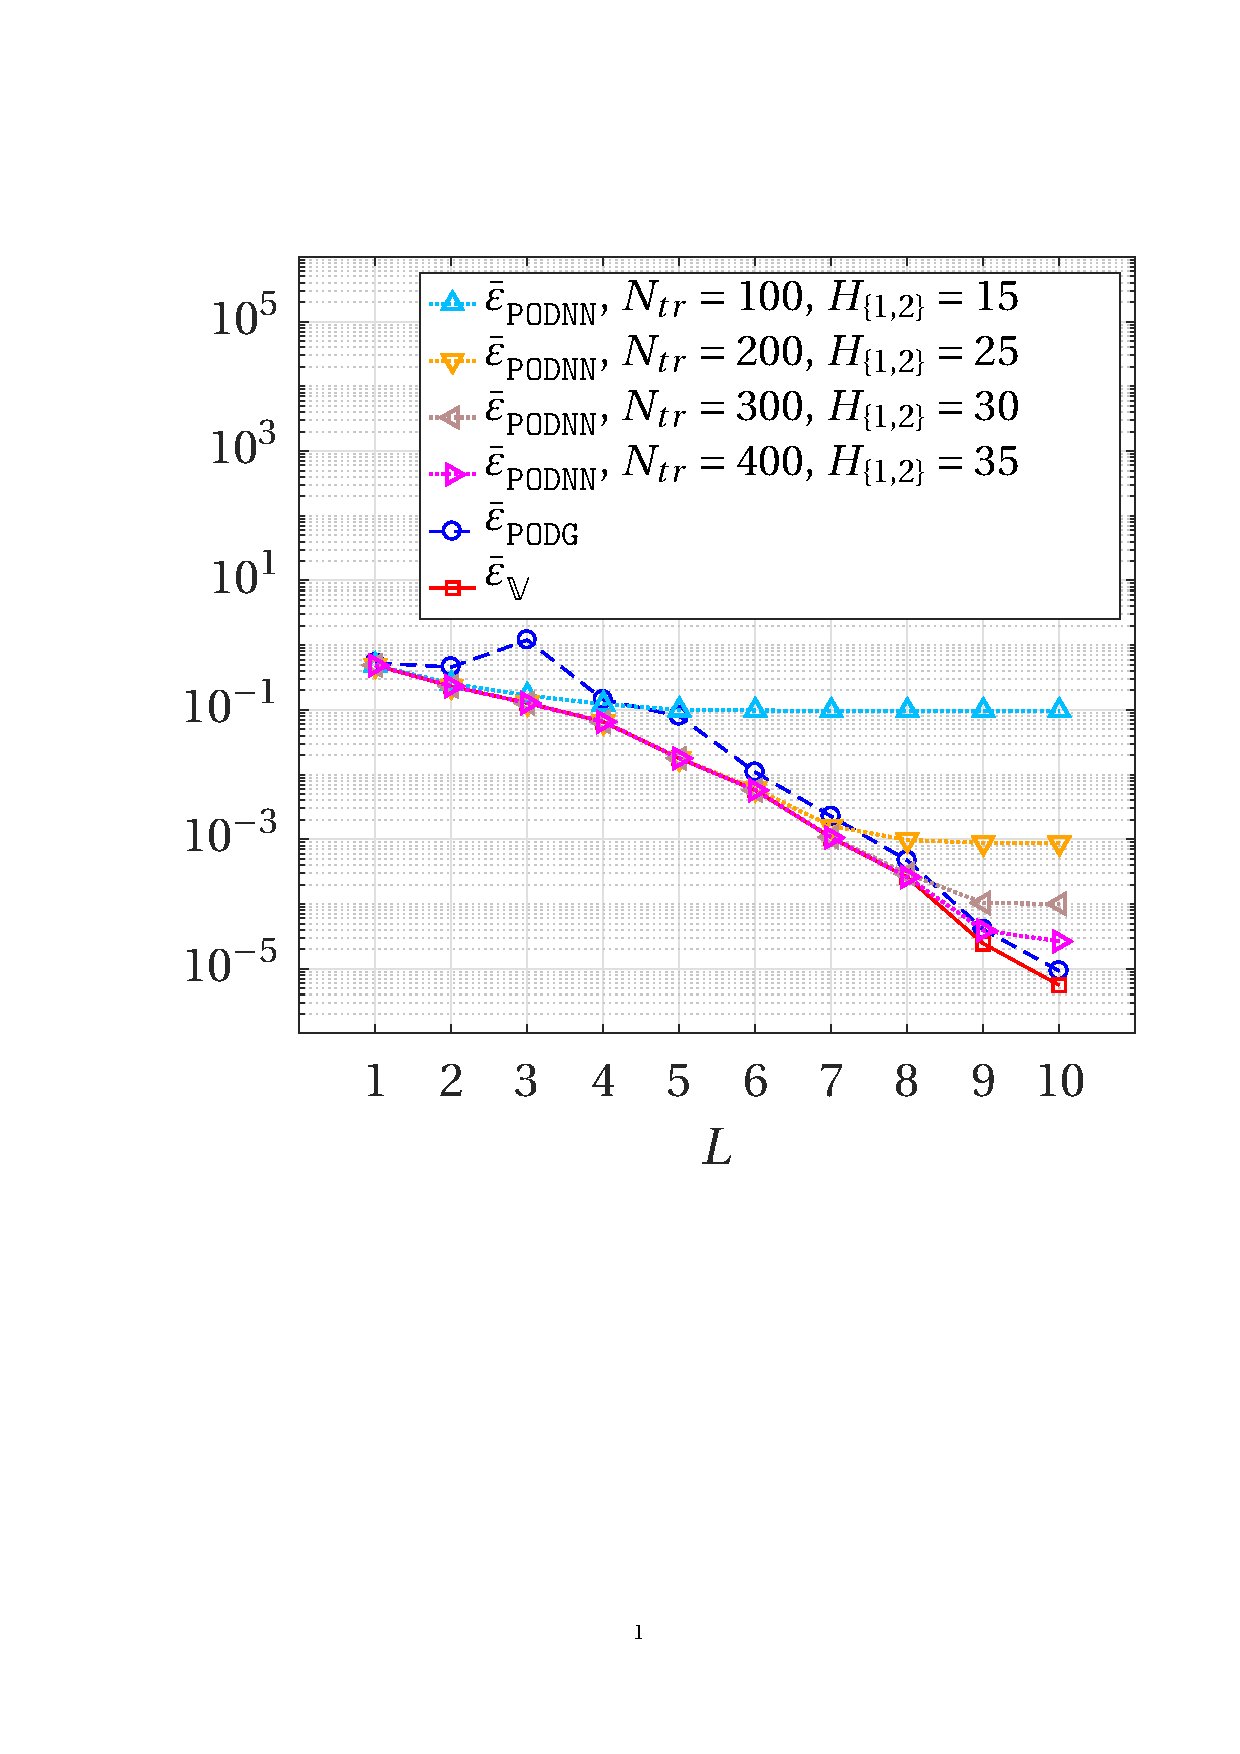
\includegraphics[scale = 0.385, trim = {1cm 9.5cm 1cm 3.5cm}, clip]{poisson1d_error_vs_rank}
			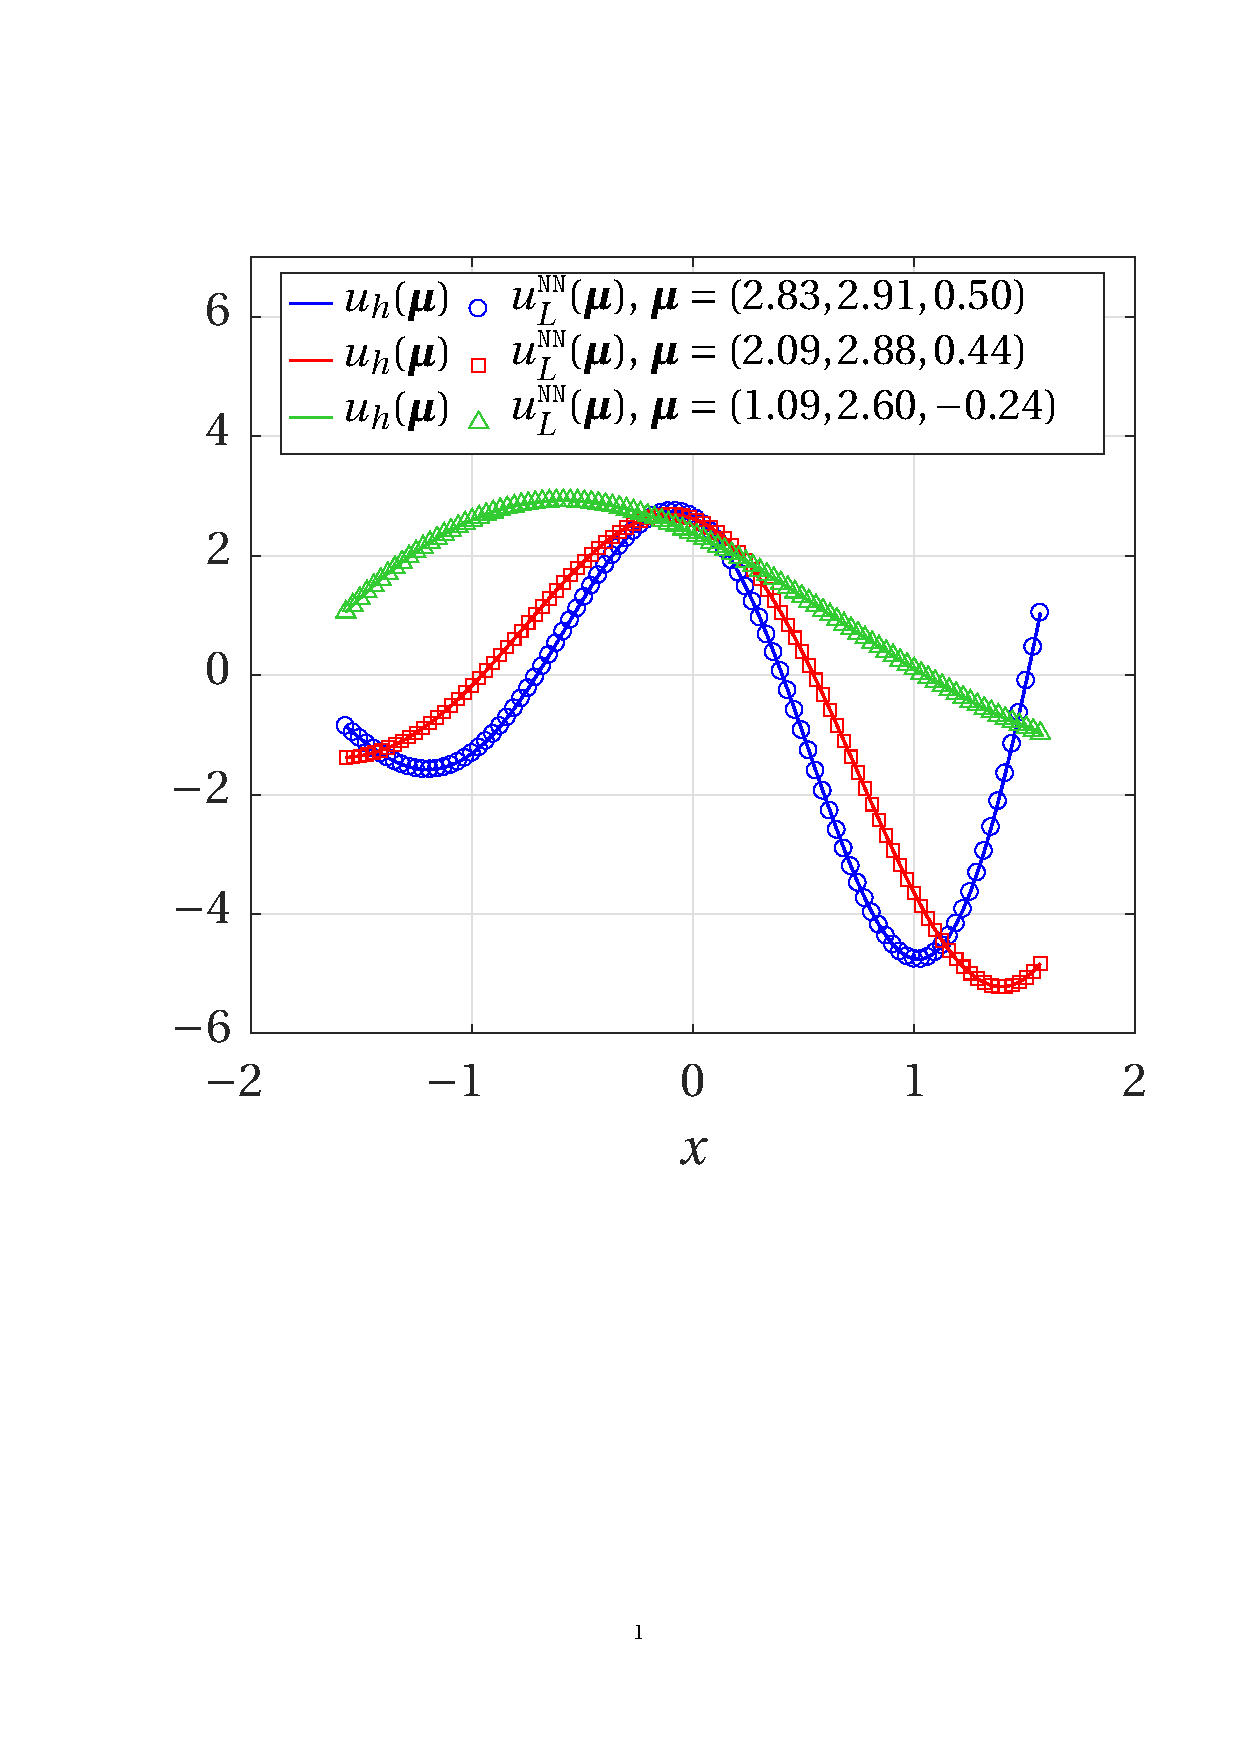
\includegraphics[scale = 0.385, trim = {1cm 9.5cm 1cm 3.5cm}, clip]{poisson1d_fe_vs_podnn}
			
			\vspace*{-0.2cm}
			
			\caption{Convergence analysis for the POD-G and POD-NN methods applied to problem \eqref{eq:poisson1d} (\emph{left}) and comparison between the FE and the POD-NN solutions for three parameter values (\emph{right}). These latter results have been obtained via a neural network with $H_1 = H_2 = 35$ units per hidden layer and employing $L = 10$ POD modes.}
			\label{fig:poisson1d-fig1}
		\end{figure}
				
		Consider the following BVP for the one-dimensional Poisson equation, featuring an exponential nonlinearity (in the diffusion coefficient) and involving three parameters:
		\vspace*{-0.2cm}
		\begin{linenomath}\begin{equation}
			\label{eq:poisson1d}
			\begin{cases}
				& - \big( \exp(u(\bg{\mu})) ~ u(\bg{\mu})' \big)' = s(x; \, \bg{\mu}) \hspace*{0.3cm} \text{in $\Omega = \left( -\dfrac{\pi}{2}, \, \dfrac{\pi}{2} \right)$} \, , \\[0.3cm]
				& u(\bg{\mu}) \big|_{x = \pm \nicefrac{\pi}{2}} = \textcolor{blue}{\mu_2 \sin\left( 2 \pm \dfrac{\mu_1 \, \pi}{2} \right) \exp \left( \pm \dfrac{\mu_3 \, \pi}{2} \right)} \, .
			\end{cases}
			\vspace*{-0.2cm}
		\end{equation}\end{linenomath}
		Here, $\bg{\mu} = \big(\mu_1, \, \mu_2, \, \mu_3 \big) \in \mathcal{P} = \big[ 1, \, 3 \big] \times \big[ 1, \, 3 \big] \times \big[ -0.5, \, 0.5 \big]$ and $s(\cdot; \bg{\mu})$ is defined such that 
		\vspace*{-0.2cm}
		\begin{linenomath}\begin{equation*}
			\textcolor{blue}{u_{ex}(x; \, \bg{\mu}) = \mu_2 \sin \big(2 + \mu_1 \, x \big) \, \exp \big( \mu_3 \, x \big)} 
			\vspace*{-0.2cm}
		\end{equation*}\end{linenomath}
		is the exact solution to the problem for any $\bg{\mu} \in \mathcal{P}$. The left plot of Fig. \ref{fig:poisson1d-fig1} shows the convergence of the POD-G and POD-NN solutions with respect to the number of basis functions $L$ retained in the model, generated via POD of $N = 100$ FE snapshots computed over a uniform mesh of $100$ nodes. Observe how the performance of the POD-NN method depends highly on the number of \textcolor{red}{training data} and hidden neurons used. In fact, for $N_{tr} = 100$ and $H_1 = H_2 = 15$ (upward-pointing triangles), the method can approximate only the first five generalized coordinates, actually providing more satisfactory results than POD-G does. Yet, the error stagnates for $L > 5$. However, as we expand the training set, we obtain more accurate predictions for a larger number of POD coefficients, provided that we allow the size of the network to increase. Particularly, employing $N_{tr} = 400$ training samples and $H_1 = H_2 = 35$ internal neurons (right-pointing triangles), the POD-NN error features an exponential decay for $L \leq 10$, resembling the projection error (squares). The reliability of the proposed RB method is also confirmed by the right plot of Fig. \ref{fig:poisson1d-fig1}, offering a comparison between the FE and POD-NN solutions for some parameter values.
				
		Diving deeper into the analysis of the POD-NN method, the leftmost plot of Fig. \ref{fig:poisson1d-fig2} offers the results concerning the search for an optimal three-layers network configuration using the methodology described in Section \ref{section:A non-intrusive RB method using neural networks}. The steps followed by the routine are represented by solid tracts; however, for the sake of completeness, we also report the test error (i.e., the minimum over multiple restarts) for any considered number of hidden neurons per layer ($H_1$ and $H_2$) and any dimension of the training set ($N_{tr}$). We remark that the basic assumption which the proposed routine relies on is fulfilled: as the number of available samples increases, the number of neurons which allows to attain the minimum error increases as well, while the minimum error itself decreases.
		
		\textcolor{red}{To motivate its employment, in the rightmost panels of Fig. \ref{fig:poisson1d-fig2} we compare the LM algorithm against two other widely-used weight-updating routines: the scaled conjugate gradient (SCG) \cite{Mol93} and the BFGS quasi-Newton method \cite{GMW81}. The comparison takes into consideration the test error (\emph{centre}) and the average training time (\emph{right}) for different amounts of training samples; the network architectures used are those suggested by the LM-based procedure analyzed above. For any considered size of the training set, LM turns out to be the most accurate method. For instance, for $N_{tr} = 400$ and $H_1 = H_2 = 35$, the average error yielded by LM is respectively two and three orders of magnitude smaller than that by BFGS and SCG. As one may expect, this comes with a cost: while BFGS requires $470~s$ and SCG only $1.1~s$, LM averagely takes $900~s$. However, we argue that the overheads associated with LM are well paid back by the large accuracy boost it guarantees. Further, recall that training is entirely performed \emph{offline} and as such it does not affect the \emph{online} running time. Yet, it is crucial to get reliable results. Hence, one should always sacrifice performance for the sake of accuracy during the offline phase, whenever resources are not constraining.}

		\begin{figure}[t!]
			\center
			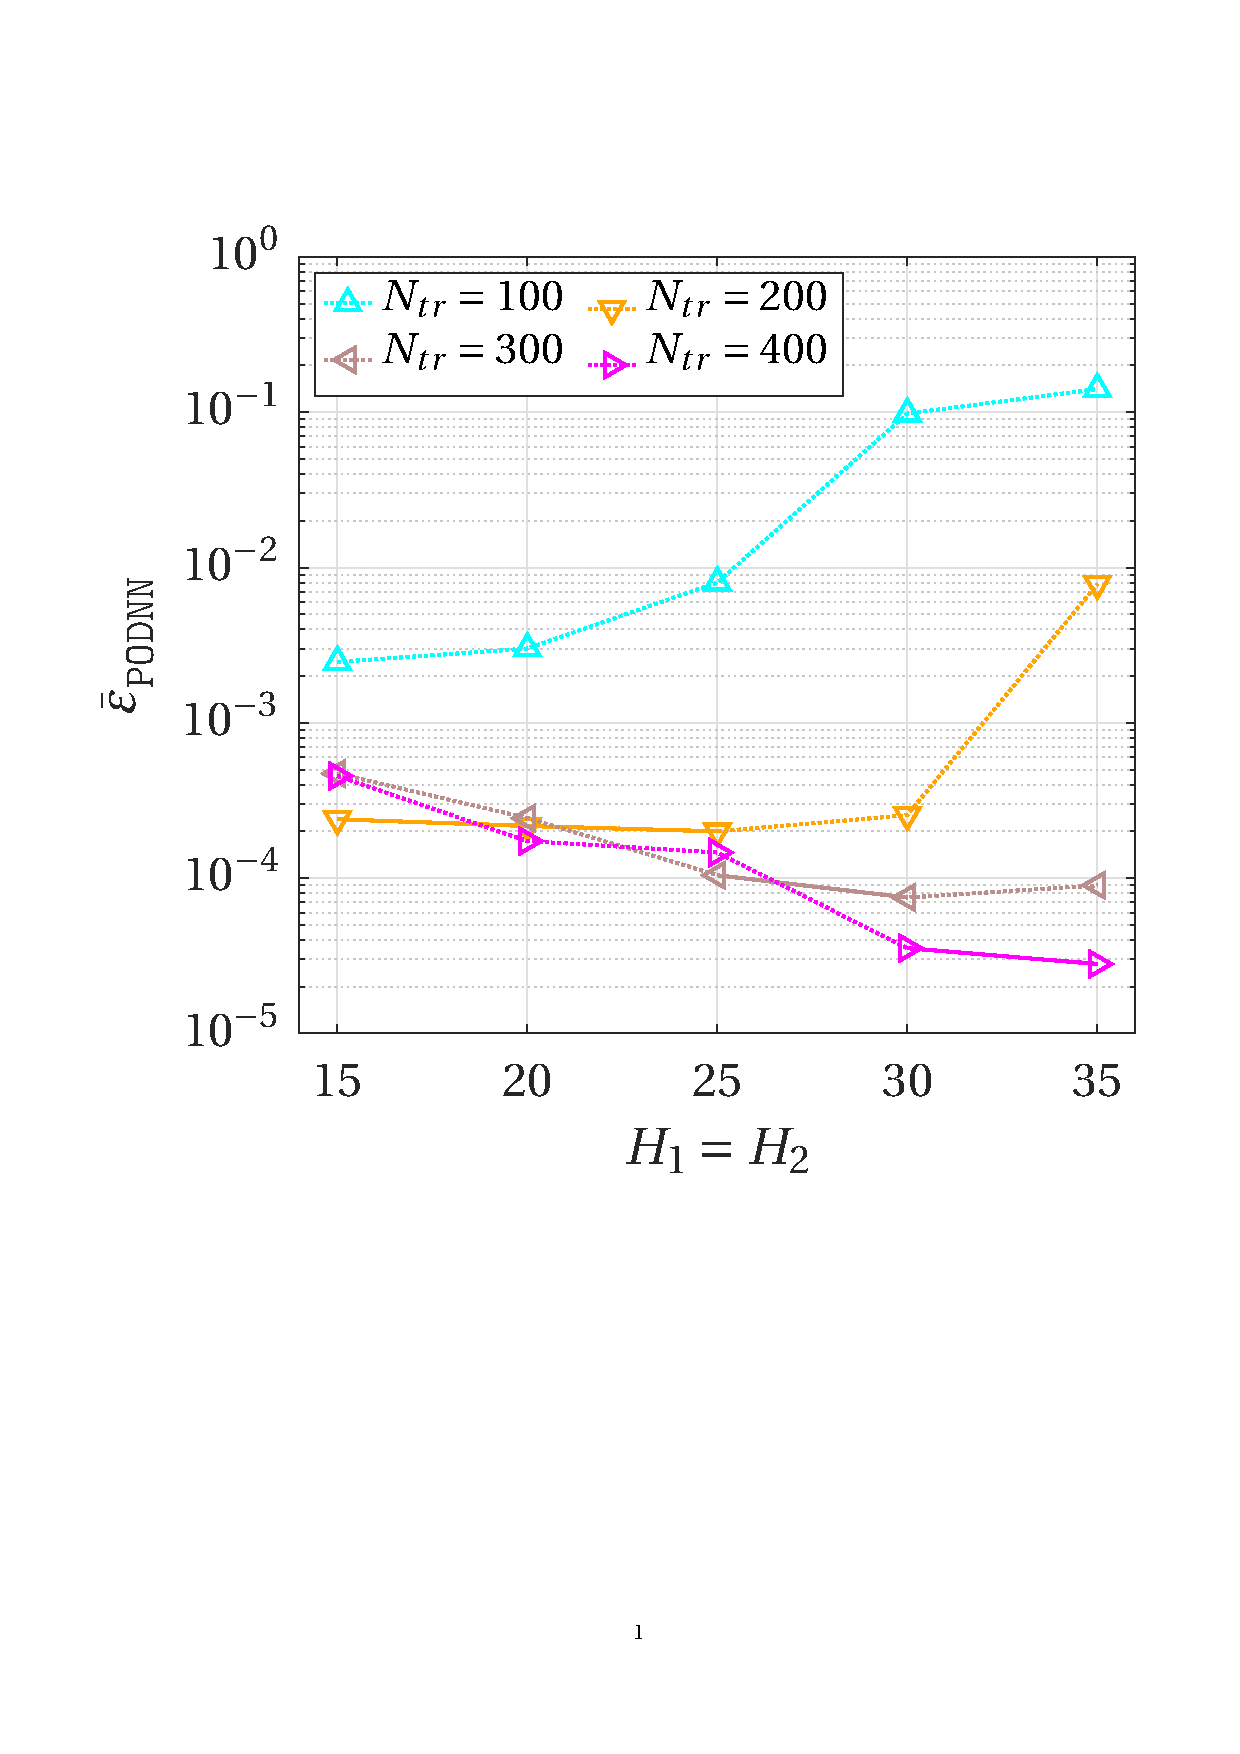
\includegraphics[scale = 0.3, trim = {1cm 9.8cm 1.5cm 3.5cm}, clip]{poisson1d_nn_convergence}
			\hspace*{0.3cm}
			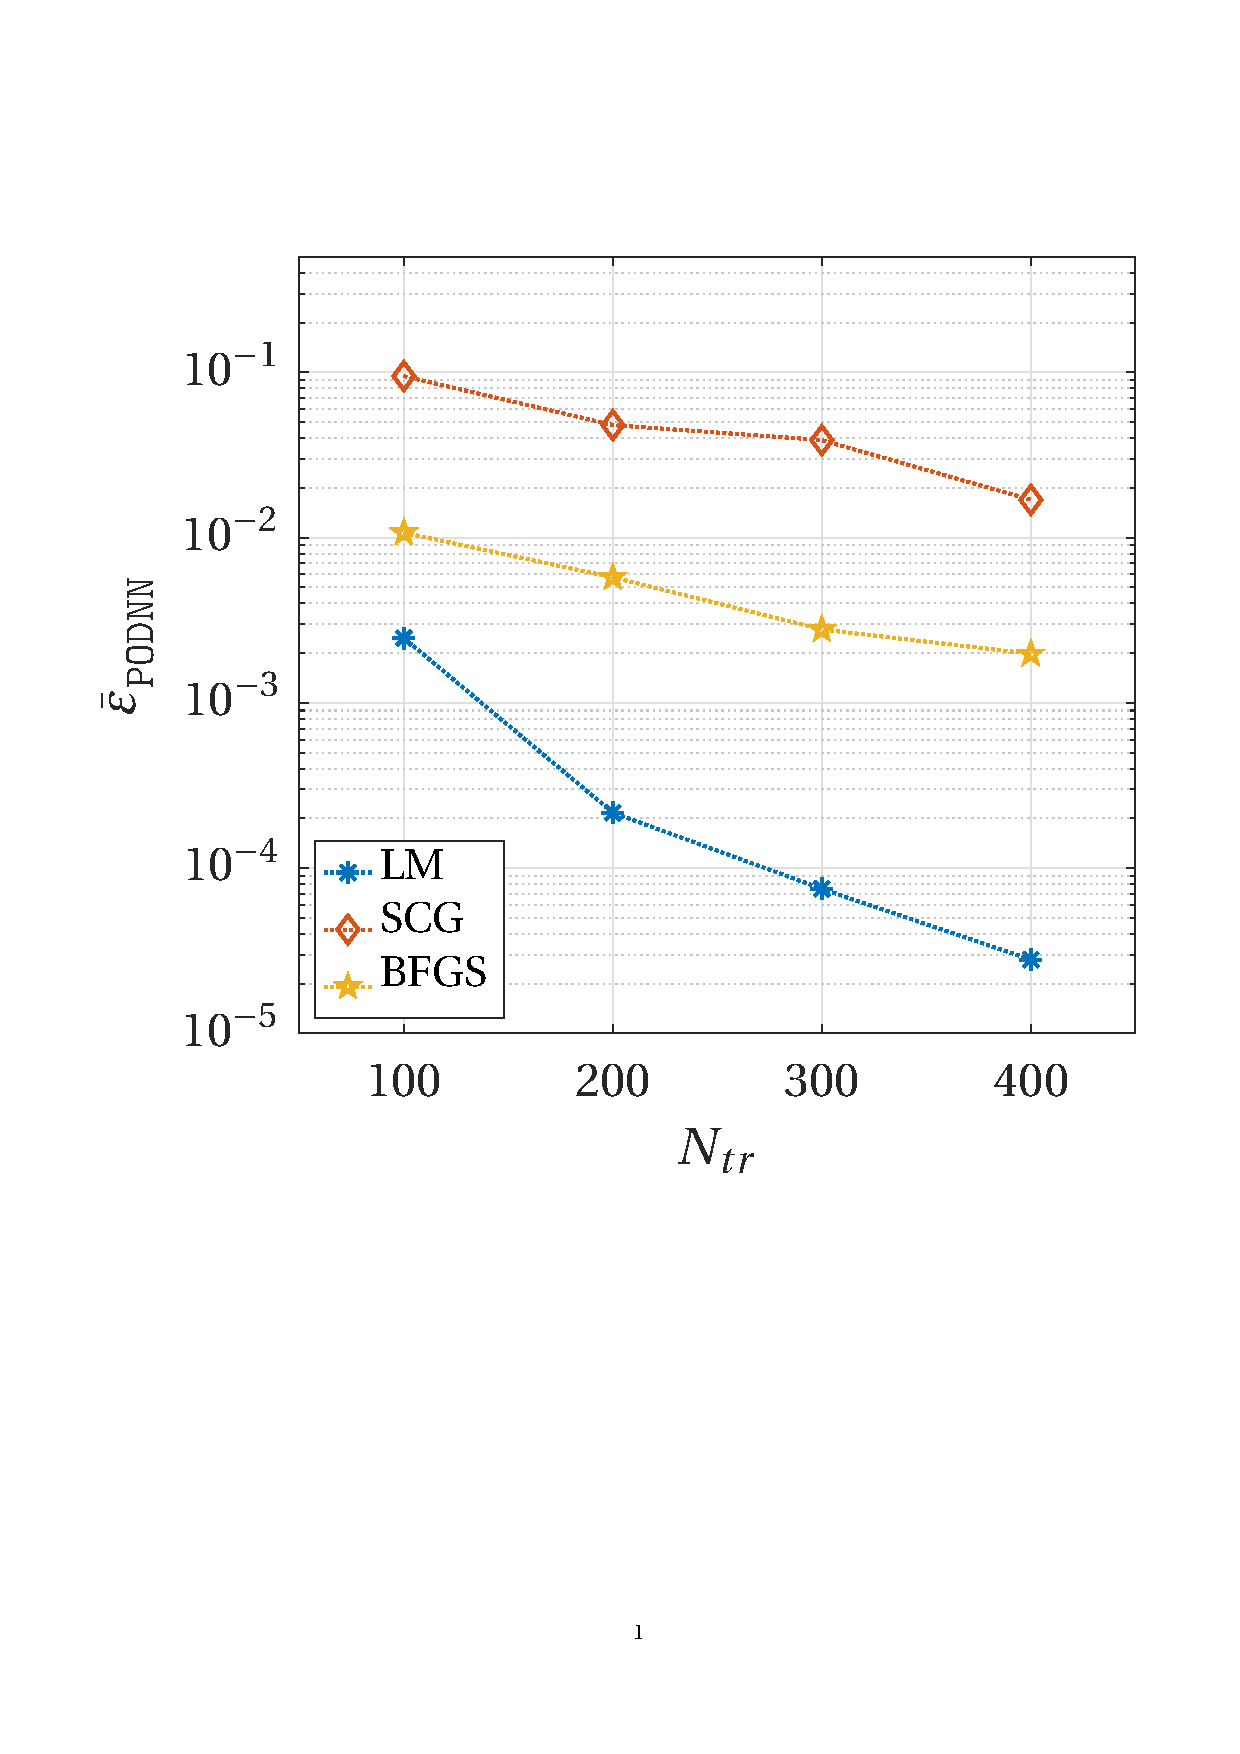
\includegraphics[scale = 0.3, trim = {1cm 9.8cm 1.5cm 3.5cm}, clip]{poisson1d_training_comparison_error}
			\hspace*{0.3cm}
			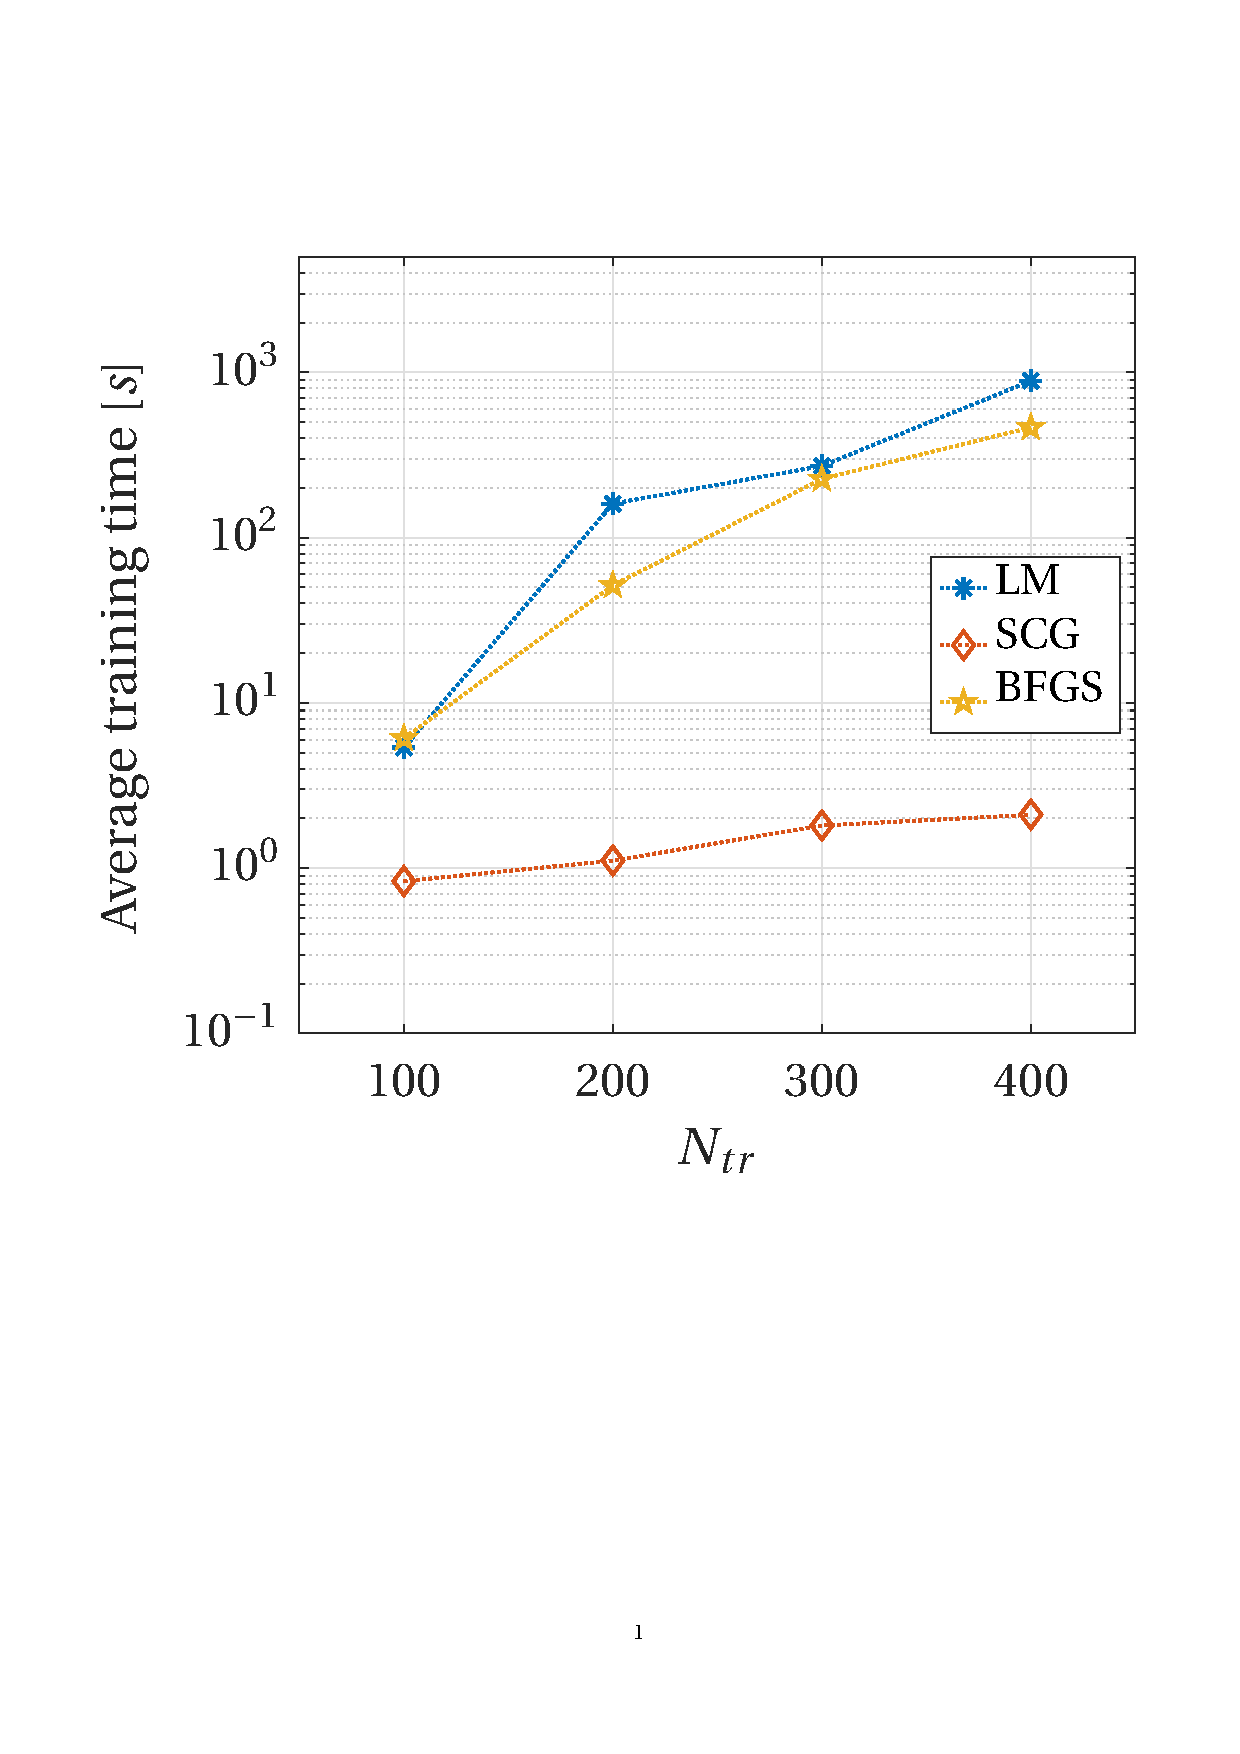
\includegraphics[scale = 0.3, trim = {1cm 9.8cm 1.5cm 3.5cm}, clip]{poisson1d_training_comparison_time}
			
			\caption{\textcolor{red}{\emph{Left}: error analysis for the POD-NN RB method applied to problem \eqref{eq:poisson1d}. Several numbers of training samples are considered; the solid sections represent the steps followed by the automatic routine described in Section \ref{section:A non-intrusive RB method using neural networks}. \emph{Centre and right}: comparison between the LM, SCG and BFGS training algorithms.}}
			\label{fig:poisson1d-fig2}
		\end{figure}
				
		
	%
	% Subsection 6.1.2 : Two-dimensional test case
	%
	
	\subsubsection{Two-dimensional test case}
	\label{section:Two-dimensional test case}
		
		\begin{figure}[b!]
			\center
			\begin{minipage}{0.4\textwidth}
				\center
				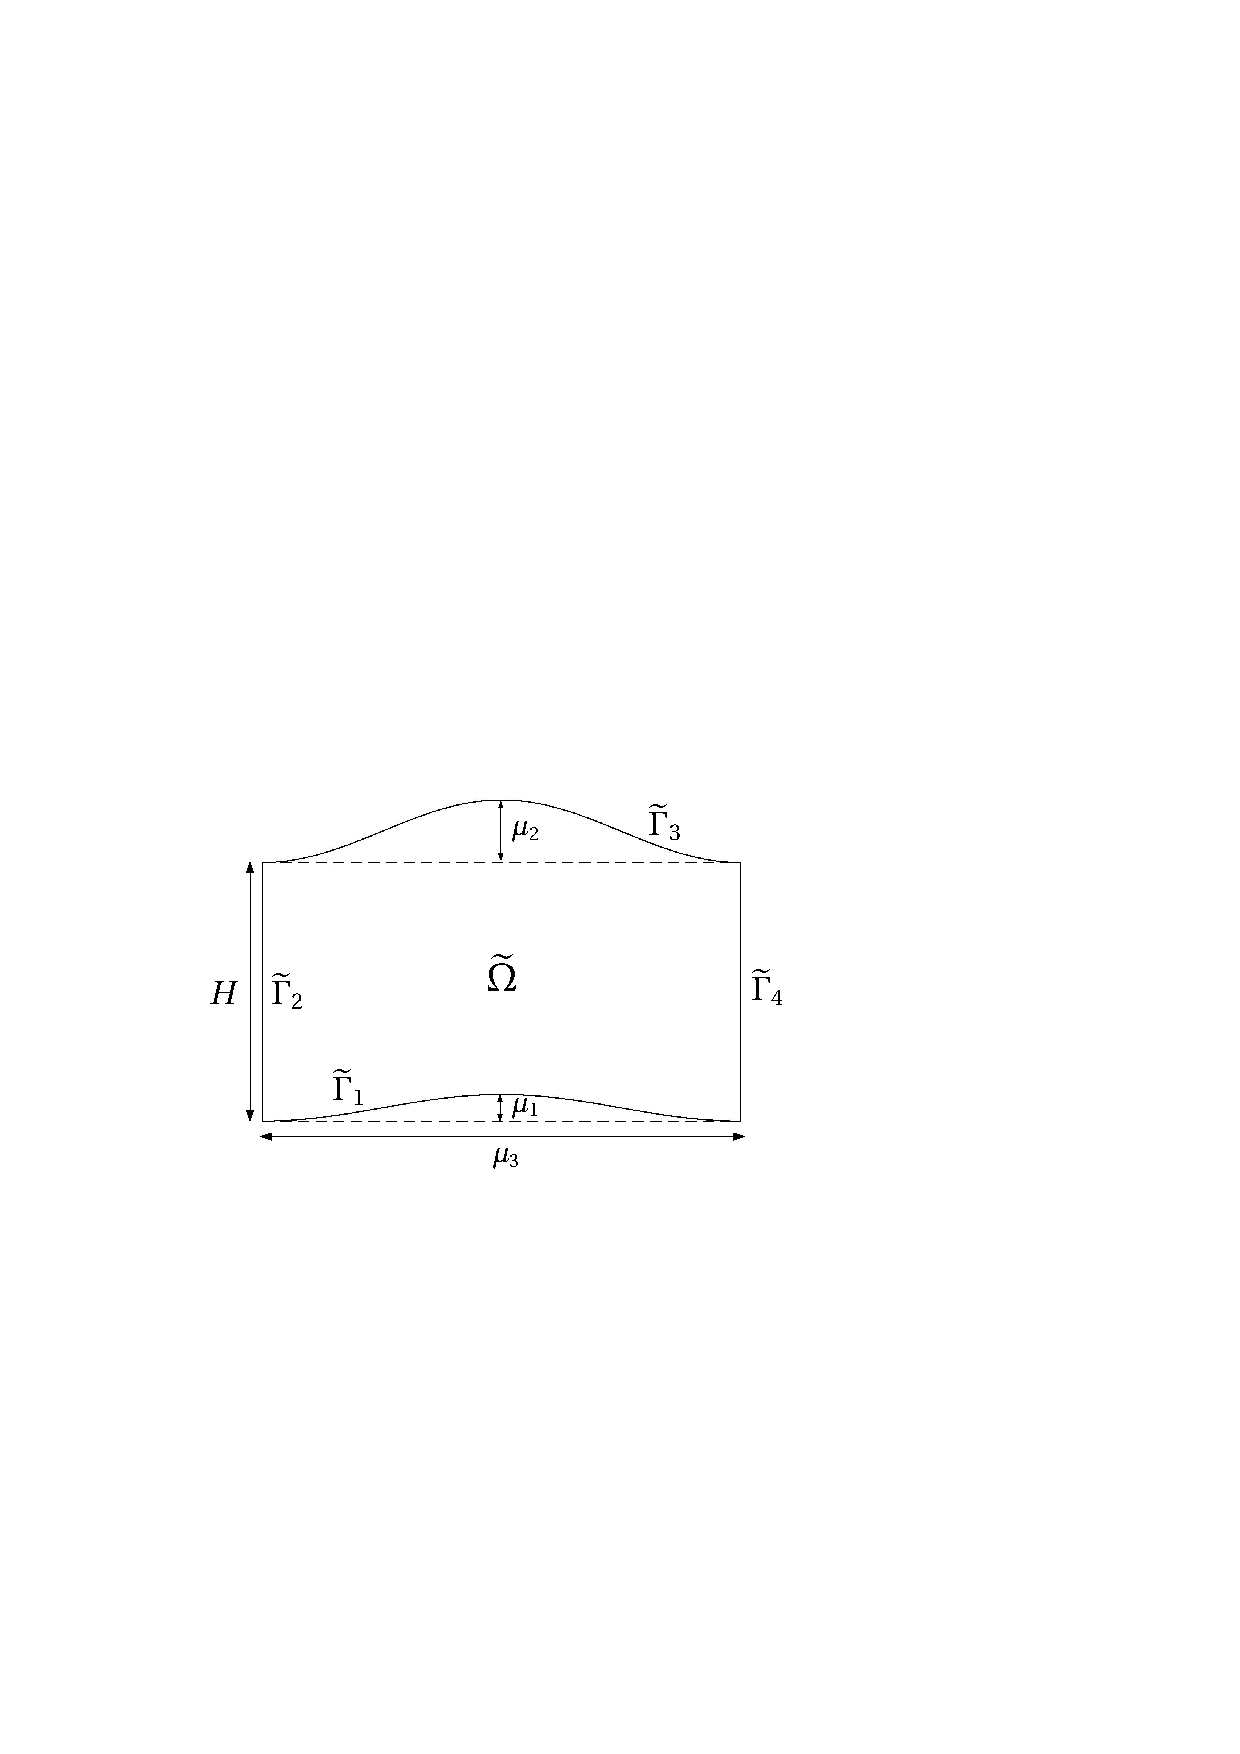
\includegraphics[scale = 0.65, trim = {0 0 0 0.5cm}, clip]{domain_stenosis} 
			\end{minipage}
			\begin{minipage}{0.4\textwidth}
				\center
				\vspace*{-0.2cm}
				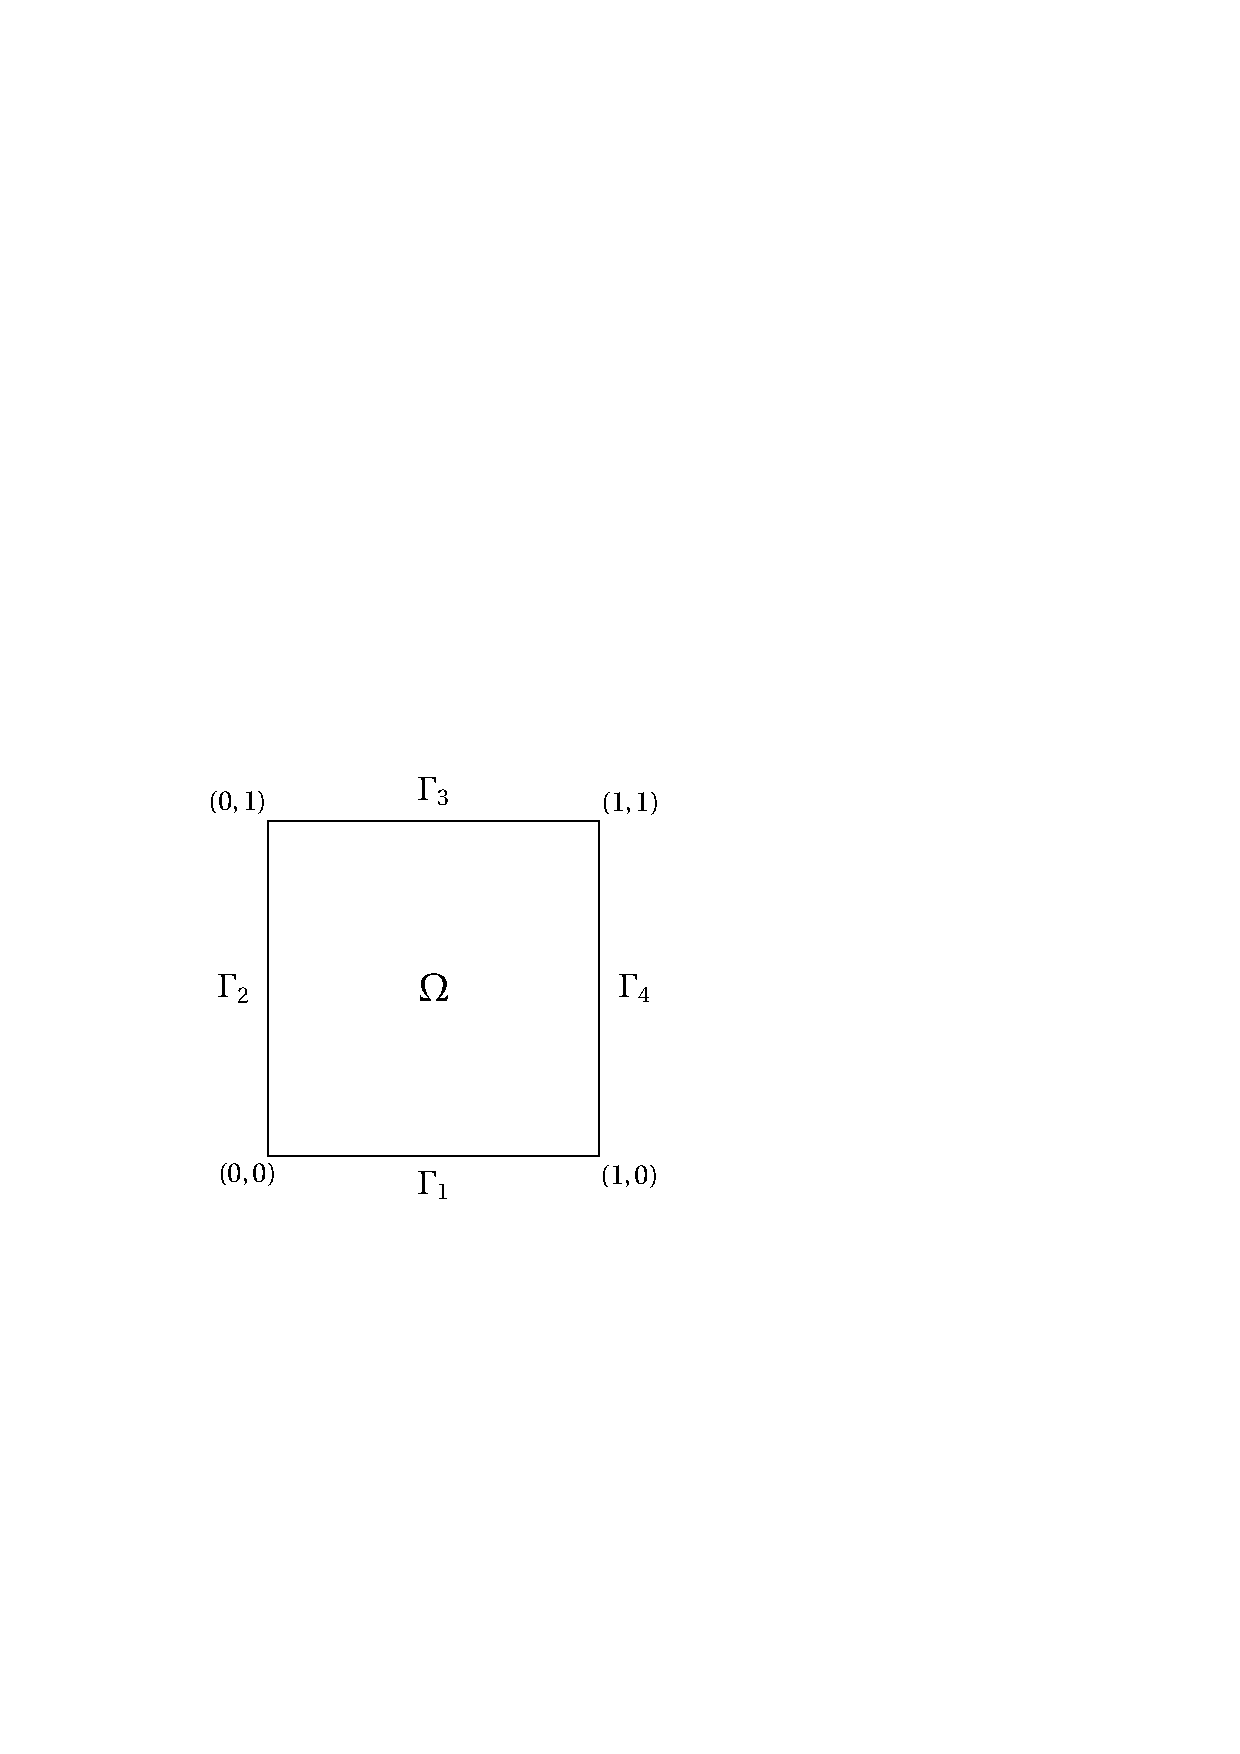
\includegraphics[scale = 0.65, trim = {0 0 0 0}, clip]{bc_square_poster}
			\end{minipage}
			
			\vspace*{-0.3cm}
			
			\caption{The physical (\emph{left}) and reference (\emph{right}) domains for the Poisson problem \eqref{eq:poisson2d}.}
			\label{fig:poisson2d-fig1}

			\vspace*{-0.1cm}

			\center
			\subfloat{\includegraphics[scale = 0.275, trim = {1cm 3cm 4cm 2.5cm}, clip]{poisson2d_fe_solution}}
			\subfloat{\includegraphics[scale = 0.275, trim = {1cm 3cm 4cm 2.5cm}, clip]{poisson2d_error_projection}} \\[-0.7cm]
			\subfloat{\includegraphics[scale = 0.275, trim = {1cm 3cm 4cm 2.5cm}, clip]{poisson2d_error_podg}}
			\subfloat{\includegraphics[scale = 0.275, trim = {1cm 3cm 4cm 2.5cm}, clip]{poisson2d_error_podnn}}
			
			%\vspace*{-0.2cm}
			
			\caption{FE solution (\emph{top left}) to the Poisson problem \eqref{eq:poisson2d} with $\bg{\mu} = (0.349, \, -0.413, \, 4.257)$, and pointwise errors yielded by either its projection onto $V_{\texttt{rb}}$ (\emph{top right}), or the POD-G method (\emph{bottom left}), or the POD-NN method (\emph{bottom right}). The results have been obtained by employing $L = 30$ POD modes.}
			\label{fig:poisson2d-fig2}
		\end{figure}

		\begin{figure}[t!]
			\center
			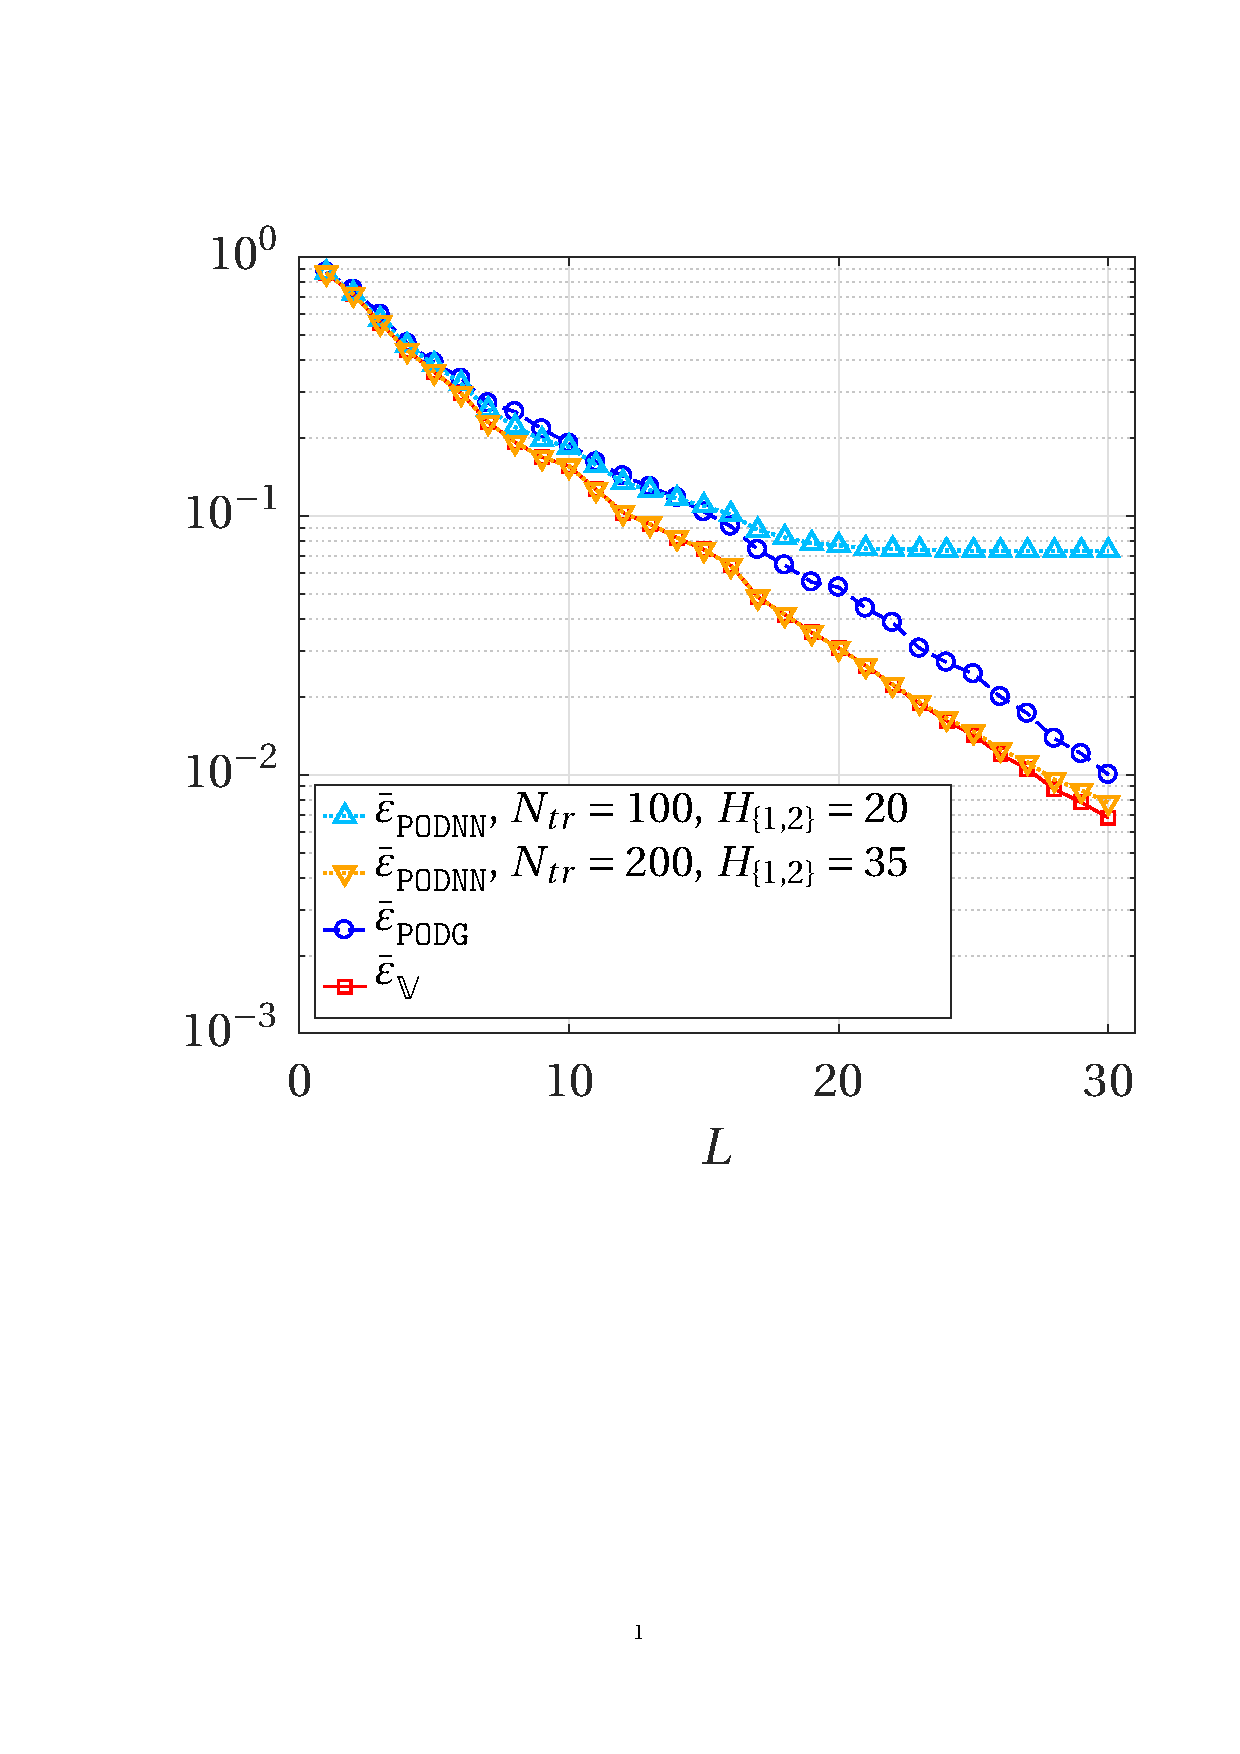
\includegraphics[scale = 0.394, trim = {1.5cm 9.6cm 1.5cm 3.8cm}, clip]{poisson2d_error_vs_rank}
			\hspace*{0.8cm}
			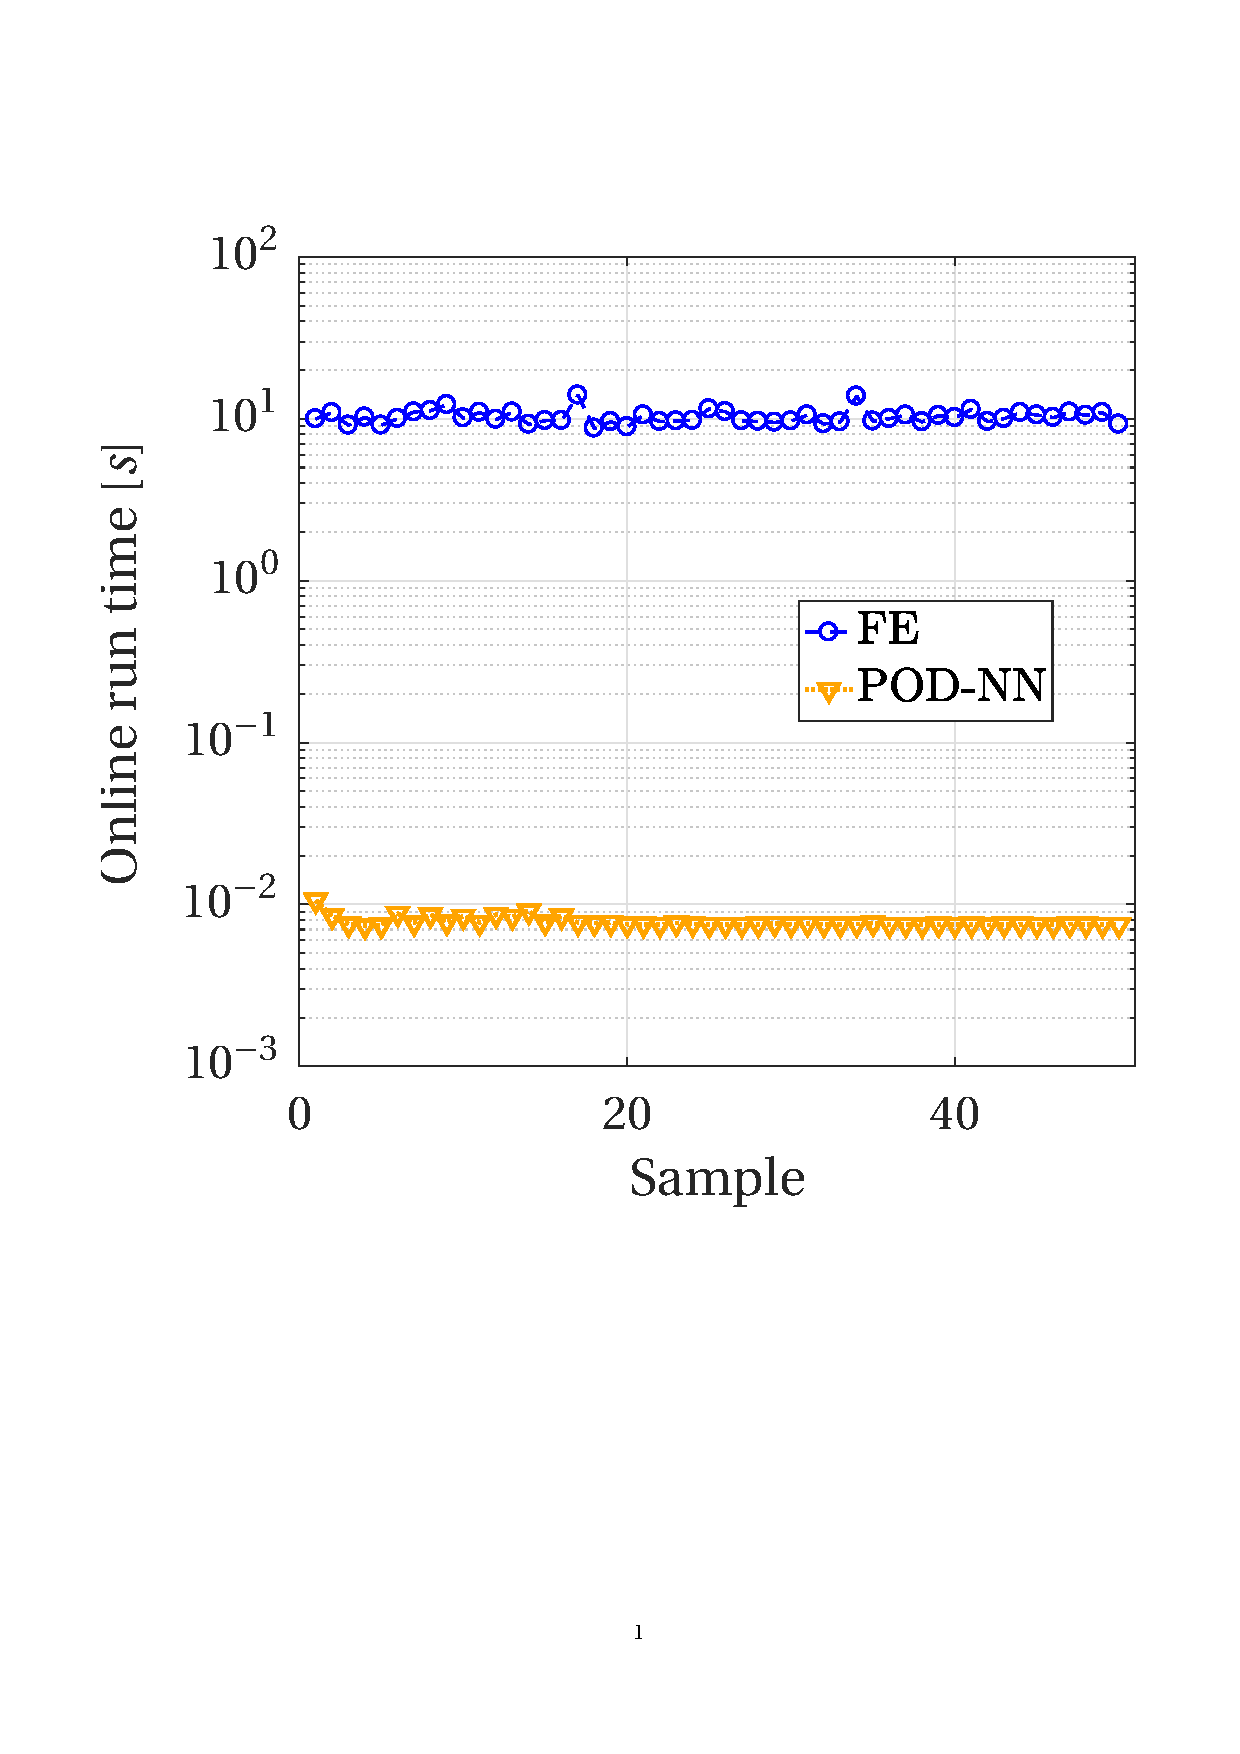
\includegraphics[scale = 0.38, trim = {1.5cm 8.95cm 1.5cm 3.8cm}, clip]{poisson2d_time}
			
			\vspace*{-0.1cm}
			
			\caption{Error analysis (\emph{left}) and online CPU time (\emph{right}) for the POD-G and the POD-NN methods applied to problem \eqref{eq:poisson2d}. The reduced basis have been generated via POD, relying on $N = 100$ snapshots. The second plot refers to RB models including $L = 30$ modal functions; within the POD-NN framework, an MLP emboding $35$ neurons per inner layer has been used.}
			\label{fig:poisson2d-fig3}
			
			\vspace*{0.3cm}
			
			\center
			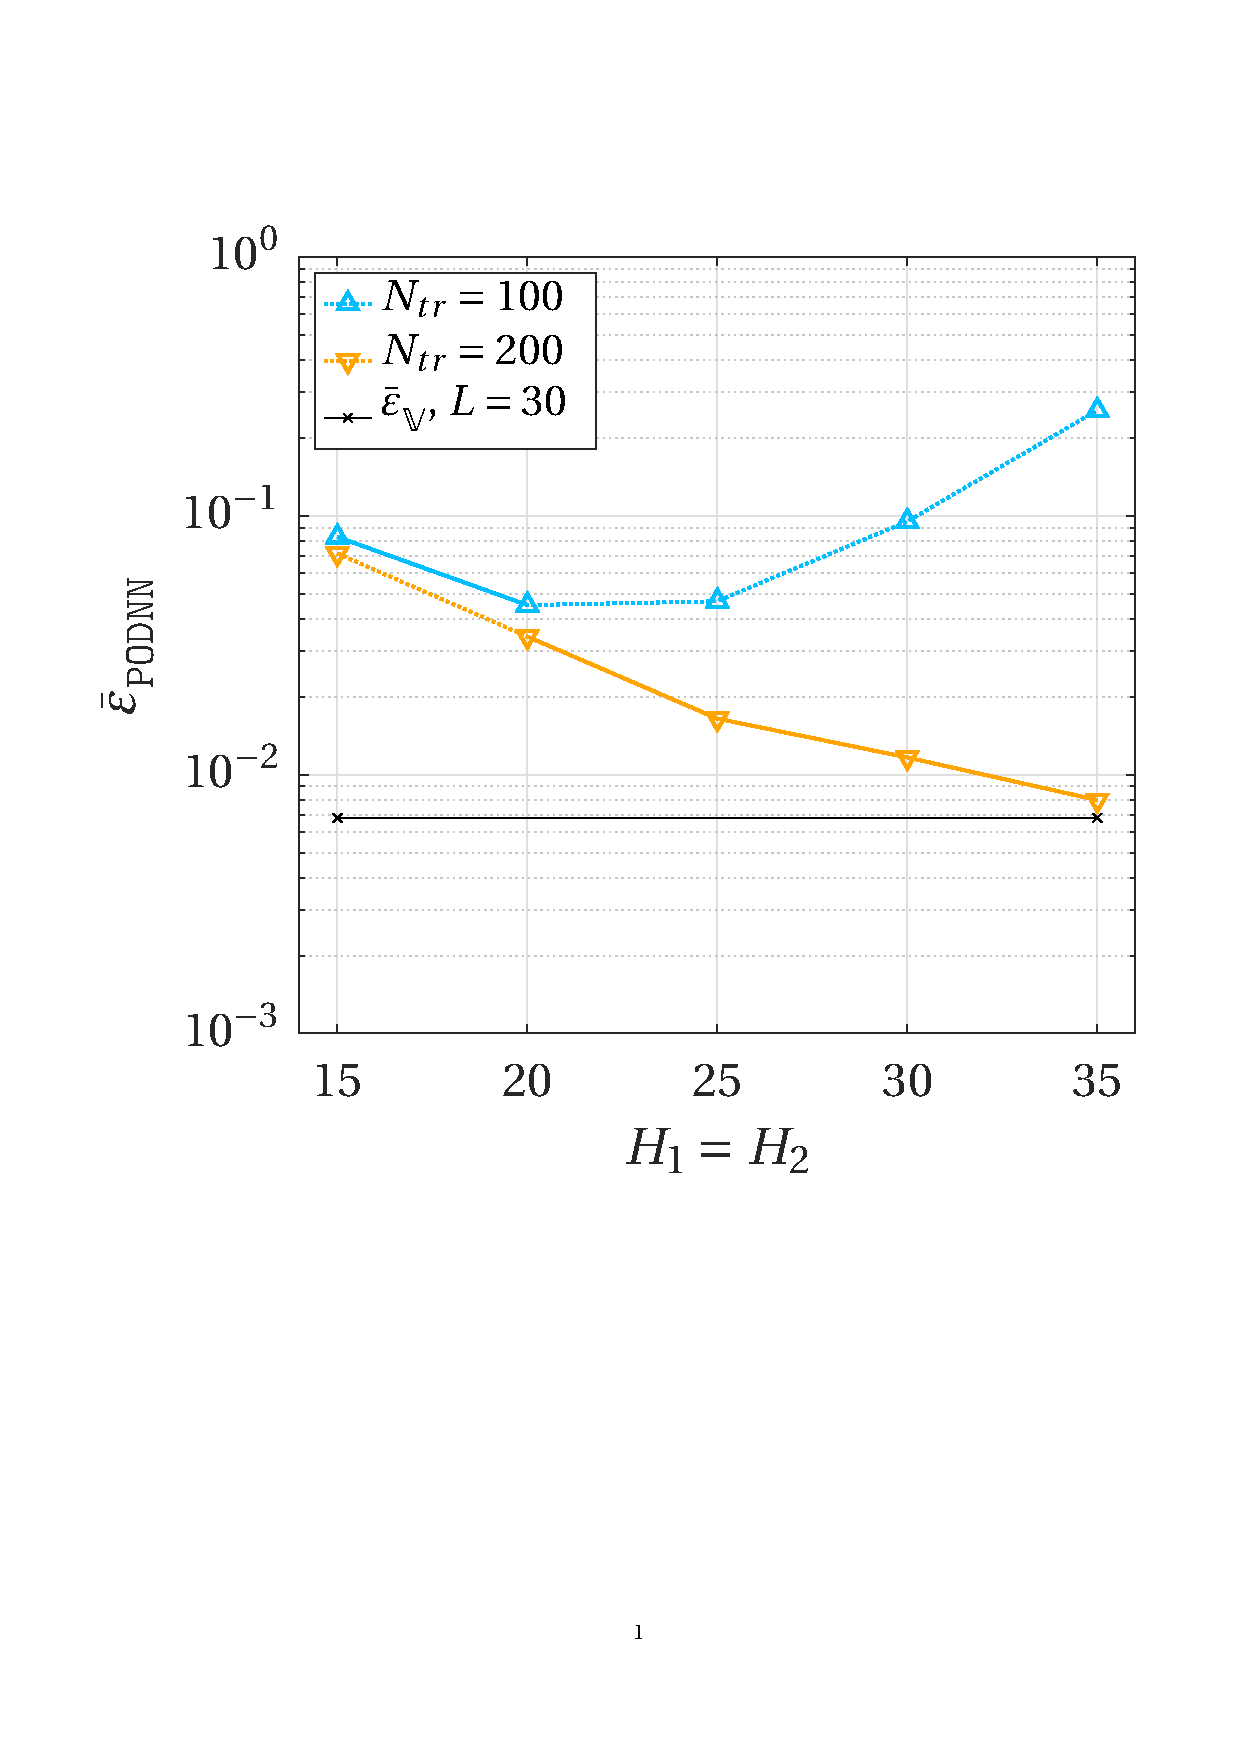
\includegraphics[scale = 0.38, trim = {1.5cm 9.6cm 1.5cm 3.8cm}, clip]{poisson2d_nn_convergence}
			\hspace*{1cm}
			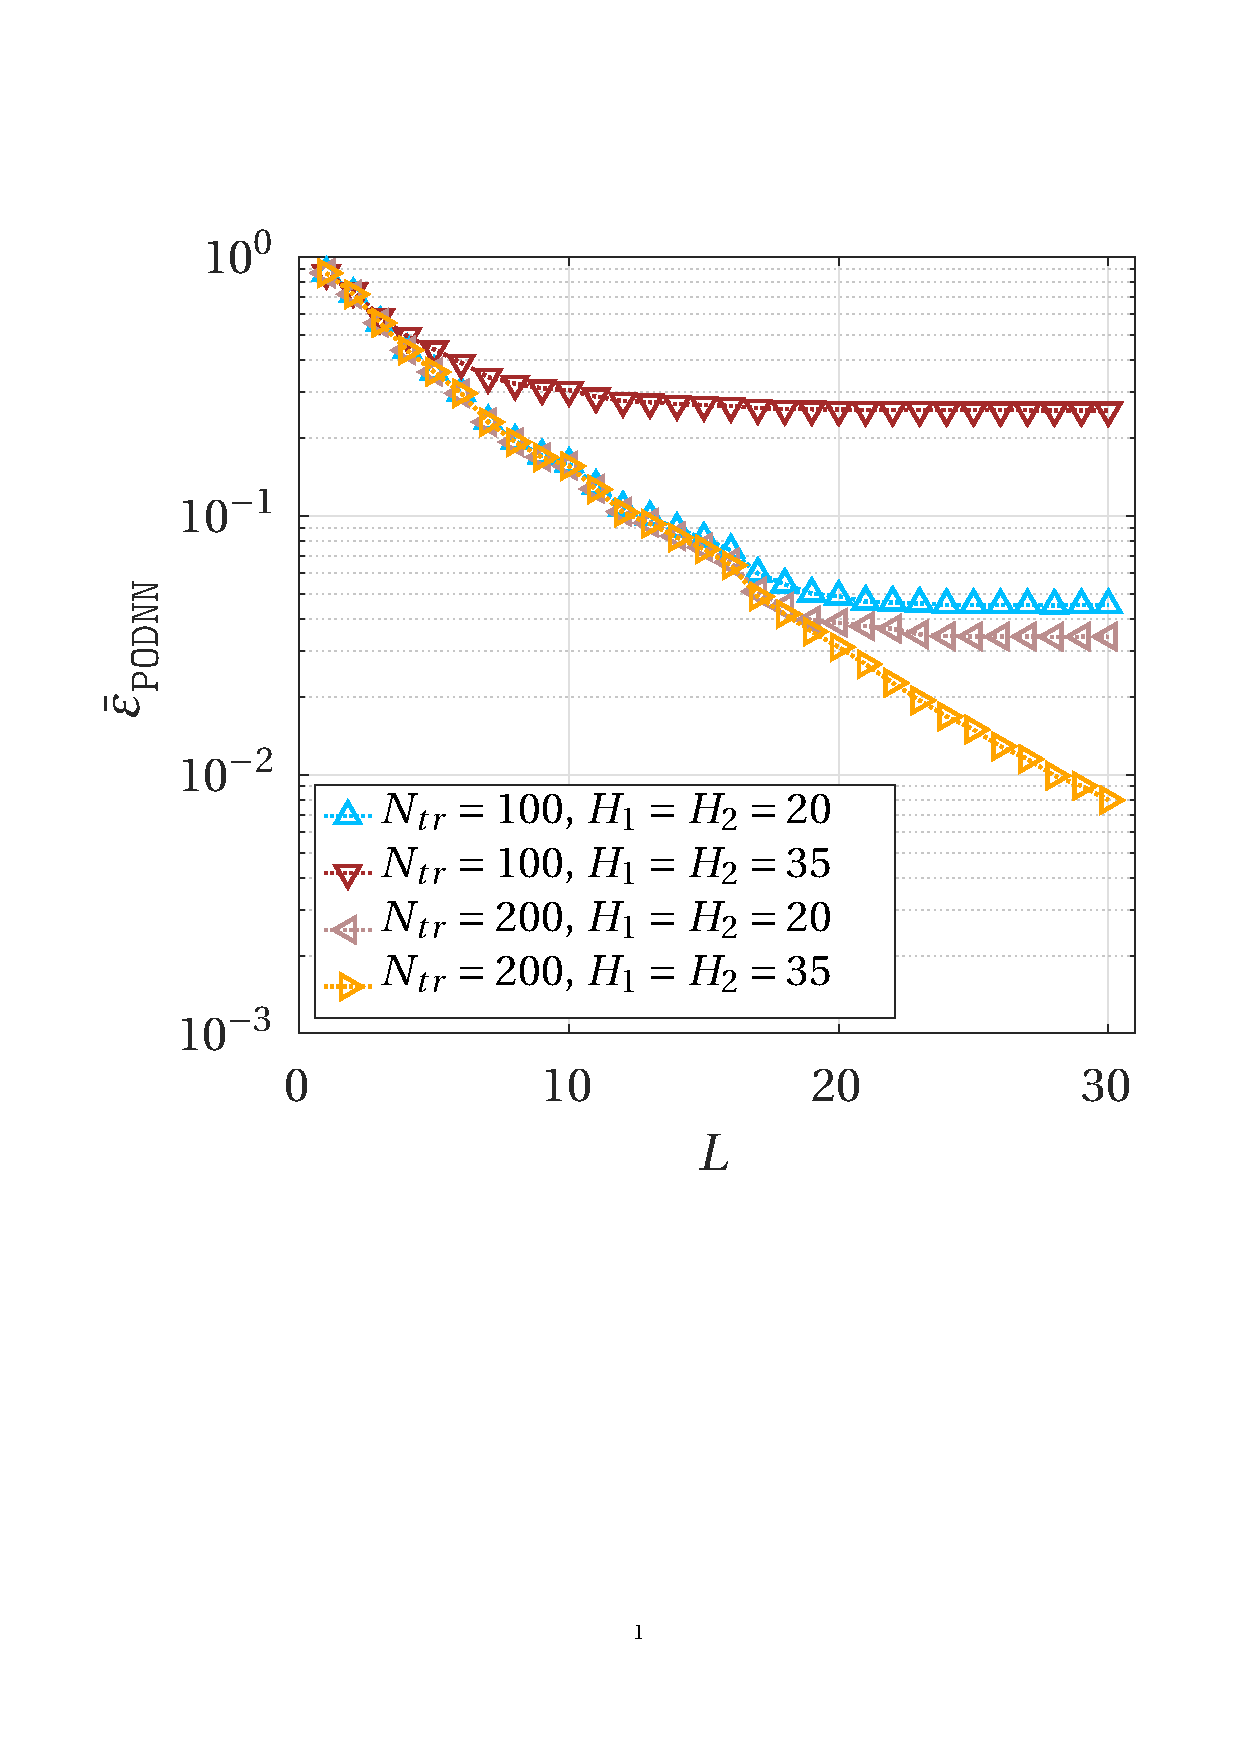
\includegraphics[scale = 0.385, trim = {1.5cm 9.8cm 1.5cm 3.8cm}, clip]{poisson2d_nn_comparison}
			
			\vspace*{-0.1cm}
						
			\caption{Convergence analysis with respect to the number of hidden neurons (\emph{left}) and modal functions (\emph{right}) used within the POD-NN framework applied to problem \eqref{eq:poisson2d}. The results provided in the first plot have been obtained using $L = 30$ modes; the solid tracts refer to the steps performed by the automatic routine carried out to find an optimal network configuration.}
			\label{fig:poisson2d-fig4}
		\end{figure}	
		Let $\bg{\mu} = [\mu_1, \, \mu_2, \, \mu_3] \in \mathcal{P} = [-0.5, \, 0.5] \times [-0.5, \, 0.5] \times [1, \, 5]$ and $\wt{\Omega}(\bg{\mu})$ be the stenosis geometry reported on the left in Fig. \ref{fig:poisson2d-fig1}, parametrized in the depths $\mu_1$ and $\mu_2$ of the bottom and top restrictions (or inflations), respectively, and the length $\mu_3$ of the vessel. The Poisson problem we deal with reads:
		\begin{linenomath}\begin{linenomath}\begin{equation}
			\label{eq:poisson2d}
			\begin{cases}
				& - \wt{\nabla} \cdot \big( \exp(\wt{u}(\bg{\mu})) ~ \wt{\nabla} \wt{u}(\bg{\mu}) \big) = \wt{s}(\wt{x}, \, \wt{y}) \hspace*{20pt} \text{in $\wt{\Omega}(\bg{\mu})$} \, , \\
				& \wt{u}(\bg{\mu}) = \wt{\sigma}_x \sin(\pi \, \wt{\sigma}_x) \cos(\pi \, \wt{\sigma}_y) \hspace*{33.5pt} \text{on $\partial \wt{\Omega}(\bg{\mu})$} \, .
			\end{cases}
		\end{equation}\end{linenomath}\end{linenomath}
		with the source term $\wt{s} = \wt{s}(\wt{x}, \, \wt{y})$ properly chosen so that the exact solution to the problem is given by \[ \wt{u}_{ex}(\wt{x}, \, \wt{y}) = \wt{y} \, \sin(\pi \, \wt{x}) \cos(\pi \, \wt{y}) \] for all $\bg{\mu} \in \mathcal{P}$. Although the state equation has an exponential nonlinearity and the computational domain presents curvilinear boundaries, both of the RB methodologies studied in this work provide accurate solutions, close to the optimal one, i.e., $u_h^{\mathbb{V}}(\bg{\mu})$.	This can be seen in Fig. \ref{fig:poisson2d-fig2}, offering the finite element solution (\emph{top left}) to \eqref{eq:poisson2d} when $\bg{\mu} = (0.349, \, -0.413, \, 4.257)$, and the pointwise errors committed by either the projection onto $V_{\texttt{rb}}$ (\emph{top right}), or the POD-G method (\emph{bottom left}), or the POD-NN method (\emph{bottom right}). The computational mesh consists of $2792$ nodes, resulting in $N_h = 2632$ degrees of freedom (as many as the inner nodes) for the FE scheme. The reduced space $V_{\texttt{rb}}$ is generated by $L = 30$ basis functions, given by POD of $N = 100$ snapshots. Specifically, the results concerning the POD-NN method have been obtained by employing a neural network equipped with $H_1 = H_2 = 35$ neurons per hidden layer and trained with $N_{tr} = 200$ learning samples. In this way, the POD-NN procedure leads to an error which shows patterns similar to those featured by the projection error. This is not surprising, due to the way neural networks are trained within the POD-NN framework (see Section \ref{section:A non-intrusive RB method using neural networks}). 
		
		
		A quantitative evidence of the efficacy of the RB approximations is given in the plot on the left in Fig. \ref{fig:poisson2d-fig3}, which reports the convergence analysis for both the POD-G and the POD-NN methods with respect to the number $L$ of retained modal basis functions. As usual, the error has to be interpreted as an average over a parameter data set $\Xi_{te}$, here consisting of $N_{te} = 50$ samples. However, the second plot of Fig. \ref{fig:poisson2d-fig3} reveals how POD-NN produces a response for any online query approximately $10^3$ times faster than POD-G does. \textcolor{red}{On the other hand, the proposed methodology implies a larger offline computational cost. Here, while generating the POD basis takes less than half an hour, the MLPs learning phase (see Fig. \ref{fig:poisson2d-fig4}, \emph{left}) lasts around $8$ hours, of which approximately one hour is devoted to compute the snapshots for training and validation.} 

		Let us further analyze the first plot of Fig. \ref{fig:poisson2d-fig3}. When the proper orthogonal decomposition of a set of $N = 100$ snapshots is coupled with a three-layers perceptron with $35$ neurons per hidden layer, trained to approximate the map \eqref{eq:map-to-approximate} relying on $N_{tr} = 200$ \textcolor{red}{learning data}, the relative error is smaller than the error committed by the POD-Galerkin procedure for each $L \leq 30$. Yet, halfing the number of \textcolor{red}{learning data} employed, the POD-NN error curve stops decreasing at $L = 20$, then incurring a plateu. In this regard, Fig. \ref{fig:poisson2d-fig4} suggests that as the size of the available training set decreases, one should reduce the amount of computing units to be embodied in the network, to limit the risk of overfitting. Particularly, when only $N_{tr} = 100$ training samples are used, the optimal network configuration comprises $20$ neurons per internal layer (\emph{left}). However, doubling the dimension of the training set, the same configuration does not allow to fully exploit the augmented amount of information. In that case, a network with, e.g., $35$ neurons per hidden layer is preferable (\emph{right}). 
	
		The distinguishing and novel feature of the POD-NN method is represented by the employment of multi-layer perceptrons to recover the coefficients of the reduced model. To motivate this choice, let us pursue a more traditional approach in the interpolation step by resorting to cubic splines \cite{Deb78}. To this end, let $\Xi_{\delta} \subset \mathcal{P}$ be a tensor-product grid on the parameter domain, based on, e.g., Chebyshev nodes. In the offline phase, for each $\bg{\mu}_{\delta} \in \Xi_{\delta}$, we compute the truth solution $\mathbf{u}_h(\bg{\mu}_{\delta}) \in \mathbb{R}^{N_h}$ and we extract the expansion coefficients $\mathbb{V}^T \mathbf{u}_h(\bg{\mu}_{\delta}) \in \mathbb{R}^L$. At the online stage, given a new parameter value $\bg{\mu} \in \mathcal{P}$, the $i$-th expansion coefficient, $i = 1, \, \ldots \, , L$, is sought by cubic spline interpolation of the samples 
		\vspace*{-0.1cm}
		\begin{linenomath}\begin{equation*}
			\big\lbrace \big( \bg{\mu}_{\delta}, \, \big( \mathbb{V}^T \mathbf{u}_h(\bg{\mu}_{\delta}) \big)_i \big) \big\rbrace_{\bg{\mu}_{\delta} \in \Xi_{\delta}} \, . 
			\vspace*{-0.1cm}
		\end{equation*}\end{linenomath}
		Hence, denoting by $\mathbf{u}_{\texttt{rb}}^{\texttt{CS}}(\bg{\mu}) \in \mathbb{R}^L$ the approximation of $\mathbb{V}^T \mathbf{u}_h(\bg{\mu})$, the reduced order approximation of $\mathbf{u}_h(\bg{\mu})$ is given by $\mathbf{u}_L^{\texttt{CS}}(\bg{\mu}) = \mathbb{V} \, \mathbf{u}_{\texttt{rb}}^{\texttt{CS}}(\bg{\mu})$. Similarly to the POD-G and the POD-NN methods, the accuracy of the resulting POD-CS procedure can be assessed by evaluating and averaging the relative error $\varepsilon_{\texttt{PODCS}}^{}(L, \, \bg{\mu})$, defined as
		\vspace*{-0.1cm}
		\begin{linenomath}\begin{equation*}
			\varepsilon_{\texttt{PODCS}}^{}(L, \, \bg{\mu}) = \dfrac{\norm{\mathbf{u}_h(\bg{\mu}) - \mathbf{u}_L^{\texttt{CS}}(\bg{\mu})}}{\norm{\mathbf{u}_h(\bg{\mu})}} = \dfrac{\norm{\mathbf{u}_h(\bg{\mu}) - \mathbb{V} \, \mathbf{u}_{\texttt{rb}}^{\texttt{CS}}(\bg{\mu})}}{\norm{\mathbf{u}_h(\bg{\mu})}} \, ,
		\end{equation*}\end{linenomath}
		on a test parameter set $\Xi_{te} \subset \mathcal{P}$, with $\Xi_{te} \cap \Xi_{\delta} = \emptyset$.
				
		\begin{figure}[b!]
			\center
			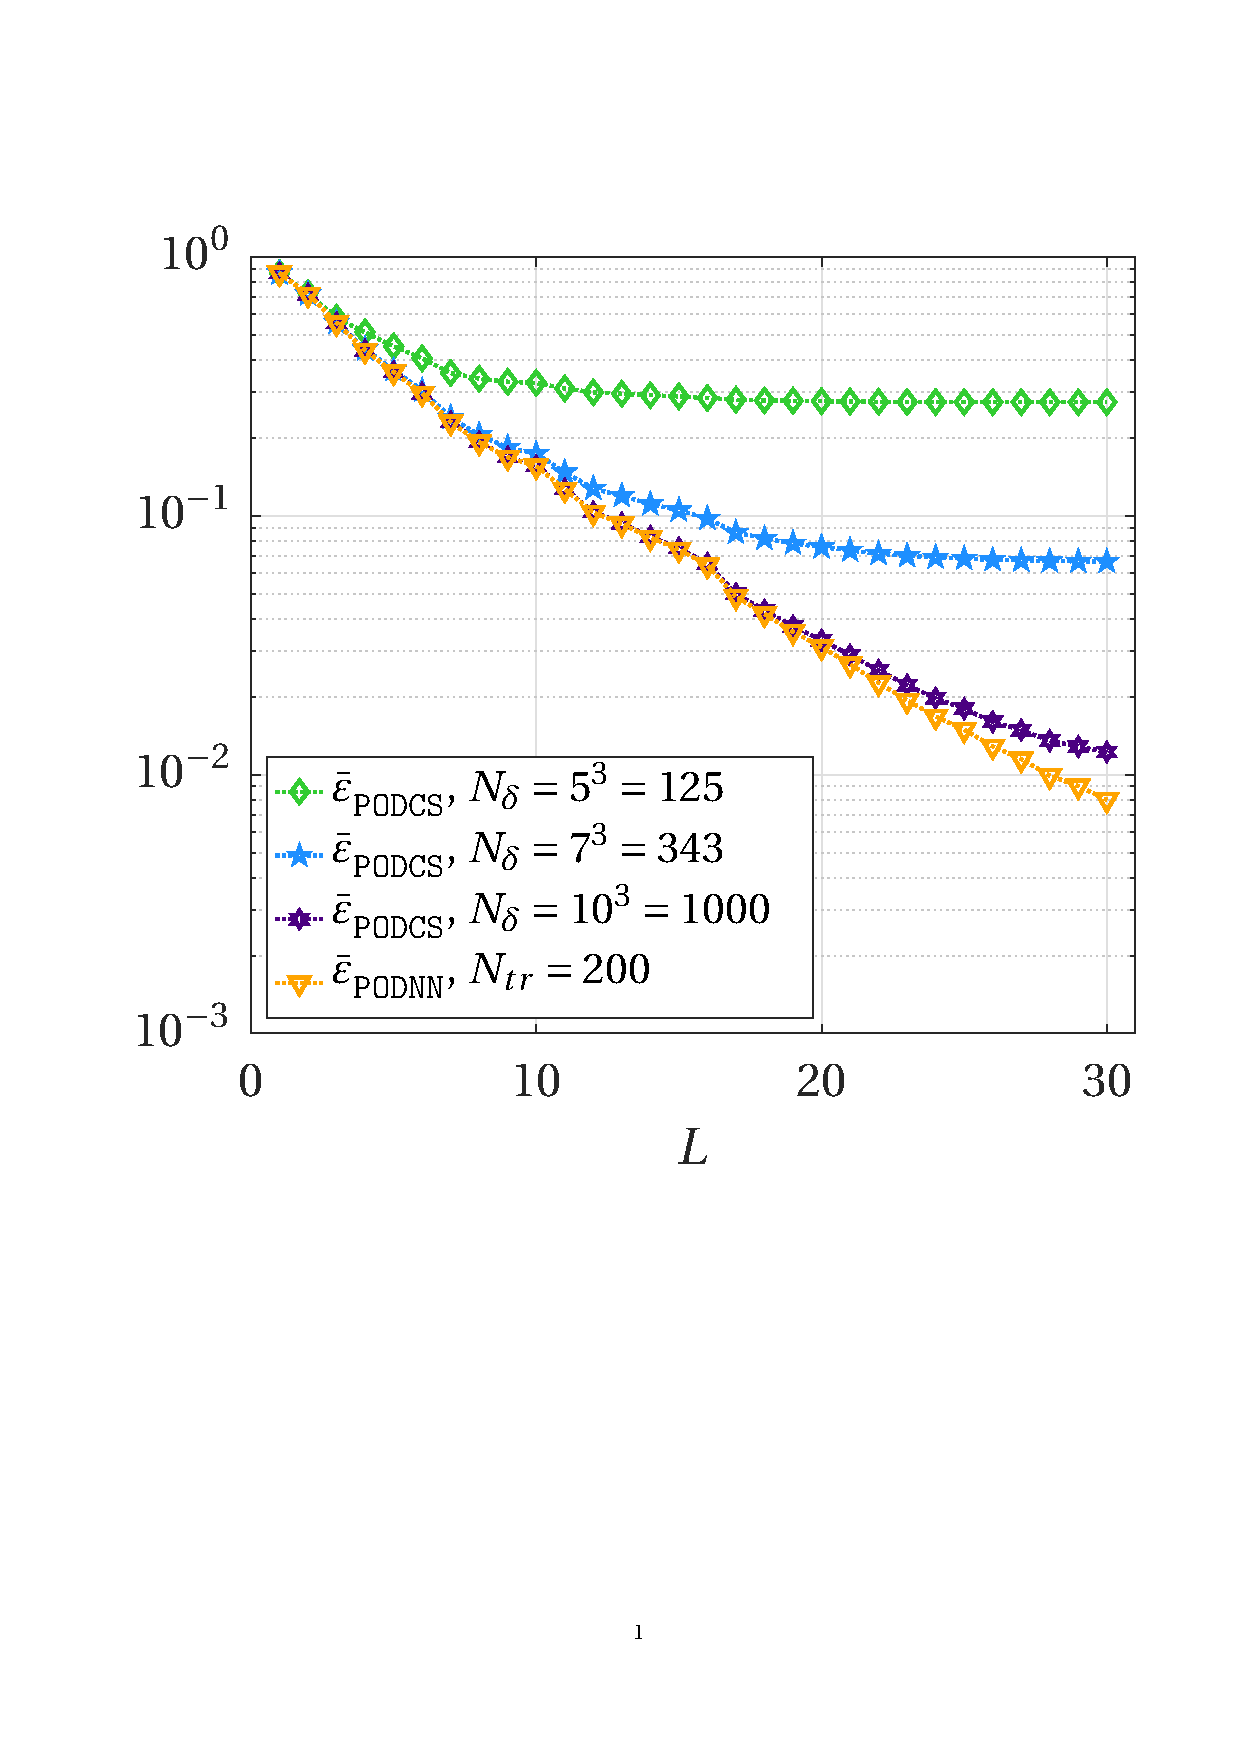
\includegraphics[scale = 0.38, trim = {1.5cm 9.34cm 1.5cm 3.8cm}, clip]{poisson2d_cs_error}
			\hspace*{1cm}
			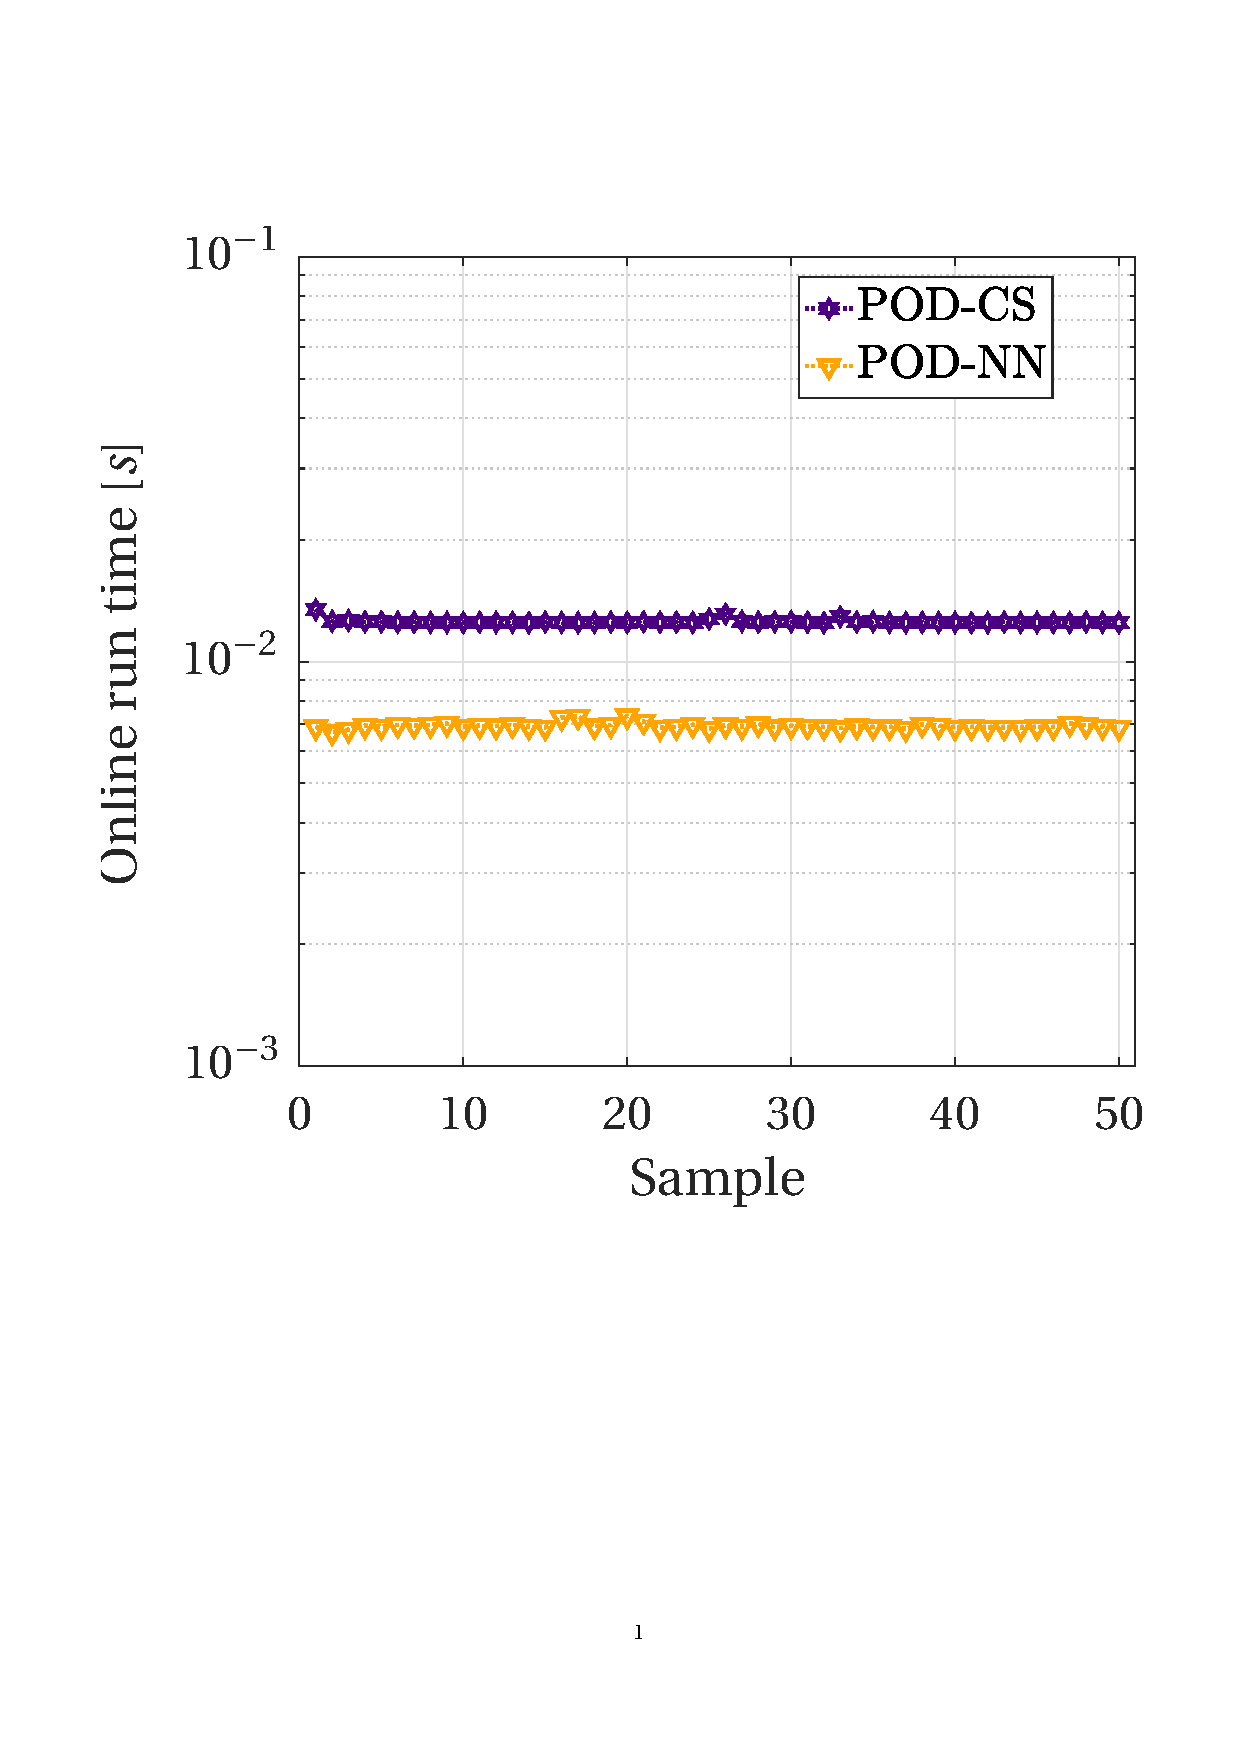
\includegraphics[scale = 0.372, trim = {1.5cm 8.9cm 1.5cm 3.8cm}, clip]{poisson2d_cs_time}
			
			\vspace*{-0.2cm}
			
			\caption{Average relative errors (\emph{left}) and online run times (\emph{right}) on $\Xi_{te}$ for the POD-CS and the POD-NN methods applied to problem \eqref{eq:poisson2d}. For the latter, the results refer to an MLP equipped with $H_1 = H_2 = 35$ neurons per hidden layer.}
			\label{fig:poisson2d-fig5}
		\end{figure}

		For the Poisson problem \eqref{eq:poisson2d}, we report in the left plot of Fig. \ref{fig:poisson2d-fig5} the relative errors by both the POD-CS and the POD-NN methods. For the former, we provide the results obtained on tensor-product grids consisting of $N_{\delta}$ interpolation points, with $N_{\delta} \in \lbrace 5^3, \, 7^3, \, 10^3 \rbrace$. For the latter, $H_1 = H_2 = 35$ neurons per hidden layer and $N_{tr} = 200$ \textcolor{red}{training data} have been used. Although the online performance of the two procedures are basically the same, as shown by the second plot in Fig. \ref{fig:poisson2d-fig5}, we observe that the level of predictive accuracy enabled by the POD-NN method can be attained or at least approached by cubic spline interpolation only when this relies on $N_{\delta} = 1000$ samples. In fact, as mentioned in the Introduction, a standard interpolation technique may require a large number of samples to be able to enforce the constraints characterizing the nonlinear manifolds which the reduced bases typically belong to \cite{Ams10}. Hence, although this approach provides a valuable alternative for paremetrized problems with a few parameters, it may be infeasible in real-life applications involving a large number of parameters. Conversely, the hope behind the choice of a neural network-based regression is that the amount of required snapshots properly scales with the dimension of the parameter space. This would justify the overheads due to the training phase.
		
		
		
	%
	% Subsection 6.2 : Steady incompressible Navier-Stokes equations
	%
		
	\subsection{Steady incompressible Navier-Stokes equations}
	\label{section:Steady incompressible Navier-Stokes equations}
	
		The system of the Navier-Stokes equations model the conservation of mass and momentum for an incompressible Newtonian viscous fluid confined in a two- or three-dimensional region \cite{Ran99}. Letting $\bg{\mu} \equiv \bg{\mu}_g$ and $\wt{\bg{v}} = \wt{\bg{v}}(\wt{\bg{x}}; \, \bg{\mu})$ and $\wt{p} = \wt{p}(\wt{\bg{x}}; \, \bg{\mu})$ be, respectively, the velocity and pressure of the fluid, the parametrized steady version of the Navier-Stokes equations considered here reads
		\begin{subequations}
			\label{eq:ns-differential}
			\begin{empheq}[left=\empheqlbrace]{align}
				\label{eq:mass-conservation}
				\wt{\nabla} \cdot \wt{\bg{v}}(\bg{\mu}) & = 0 & \hspace*{-2cm} \text{in $\wt{\Omega}(\bg{\mu})$} \, , \\
				\label{eq:momentum-conservation}
				- \nu(\bg{\mu}) ~ \wt{\Delta} \wt{\bg{v}}(\bg{\mu}) + (\wt{\bg{v}}(\bg{\mu}) \cdot \wt{\nabla}) \wt{\bg{v}}(\bg{\mu}) + \dfrac{1}{\rho(\bg{\mu})} \wt{\nabla} \wt{p}(\bg{\mu}) & = \bg{0} & \hspace*{-2cm} \text{in $\wt{\Omega}(\bg{\mu})$} \, , \\
				\wt{\bg{v}}(\bg{\mu}) & = \wt{\bg{h}} & \hspace*{-2cm} \text{on $\wt{\Gamma}_D(\bg{\mu})$} \, , \\
				\wt{p}(\bg{\mu}) \wt{\bg{n}} - \nu(\bg{\mu}) \wt{\nabla} \wt{\bg{v}}(\bg{\mu}) \cdot \wt{\bg{n}} & = \bg{0} & \hspace*{-2cm} \text{on $\wt{\Gamma}_N(\bg{\mu})$} \, .
			\end{empheq}
		\end{subequations}
		Here, $\wt{\bg{h}}$ denotes the velocity field prescribed on $\wt{\Gamma}_D(\bg{\mu})$, whereas homogeneous Neumann conditions are applied on $\wt{\Gamma}_N(\bg{\mu})$. Furthermore, $\rho(\bg{\mu})$ and $\nu(\bg{\mu})$ represent the uniform density and kinematic viscosity of the fluid, respectively. Note that, despite that these quantities encode physical properties, we let them depend on the geometrical parameters as well. Indeed, fluid dynamics can be characterized (and controlled) by means of a wealth of dimensionless quantities, e.g., the Reynold's number, which combine physical properties of the fluid with geometrical features of the domain. Therefore, a numerical study of the sensitivity of the system \eqref{eq:ns-differential} with respect to $\bg{\mu}$ may be carried out by adapting either $\rho(\bg{\mu})$ or $\nu(\bg{\mu})$ as $\bg{\mu}$ varies, so to preserve a dimensionless quantity of interest.
		
		To write the differential system \eqref{eq:ns-differential} in weak form over a $\bg{\mu}$-independent configuration $\Omega$, let us introduce the velocity and pressure spaces \[ \wt{X}(\bg{\mu}) = \big[ H^1_{\wt{\Gamma}_D} \big( \wt{\Omega}(\bg{\mu}) \big) \big]^d ~~ \text{and} ~~ \wt{Q}(\bg{\mu}) = L^2 \big( \wt{\Omega}(\bg{\mu}) \big) \, , \] respectively, with \[ X = \big[ H^1_{\Gamma_D} \big( \Omega \big) \big]^d ~~ \text{and} ~~ Q = L^2 \big( \Omega \big) \] be their respective counterparts over $\Omega$. By multiplying \eqref{eq:ns-differential} by test functions $\big( \wt{\bg{\chi}}, \, \wt{\xi} \big) \in \wt{V}(\bg{\mu}) = \wt{X}(\bg{\mu}) \times \wt{Q}(\bg{\mu})$, integrating by parts and then tracing everything back onto $\Omega$ by means of the parametrized map $\bg{\Phi}(\cdot; \, \bg{\mu})$, we end up with the following parametrized weak variational problem: given $\bg{\mu} \in \mathcal{P}$, find $u(\bg{\mu}) = (\bg{v}(\bg{\mu}), \, p(\bg{\mu})) \in V = X \times Q$ so that
		\vspace*{-0.1cm}
		\begin{linenomath}\begin{equation*}
			\begin{aligned}
				a(\bg{v}(\bg{\mu}), \, \bg{\chi}; \, \bg{\mu}) + c(\bg{v}(\bg{\mu}), \, \bg{v}(\bg{\mu}), \, \bg{\chi}; \, \bg{\mu}) + d(\bg{v}(\bg{\mu}), \, \bg{\chi}; \, \bg{\mu}) + b(p(\bg{\mu}), \, \nabla \cdot \bg{\chi}; \, \bg{\mu}) & = f_1(\bg{\chi}; \, \bg{\mu}) \, , \\
				b(\nabla \cdot \bg{v}(\bg{\mu}), \, \xi; \, \bg{\mu}) & = f_2(\xi; \, \bg{\mu}) \, ,
			\end{aligned}
		\end{equation*}\end{linenomath}
		for all $(\bg{\chi}, \, \xi) \in V$, with, for any $\bg{\mu} \in \mathcal{P}$,	
		\vspace*{-0.1cm}	
		\begin{linenomath}\begin{equation*}
			\begin{aligned}
				& c(\bg{\psi}, \, \bg{\chi}, \, \bg{\eta}; \, \bg{\mu}) = \int_{\Omega} \left( \bg{\psi} \cdot \mathbb{J}^{-T}_{\bg{\Phi}}(\bg{\mu}) \nabla \right) \bg{\chi} \cdot \bg{\eta} ~ \lvert \mathbb{J}_{\bg{\Phi}}(\bg{\mu}) \rvert \, d \Omega \, , \qquad && d(\bg{\psi}, \, \bg{\chi}; \, \bg{\mu}) = c(\bg{l}(\bg{\mu}), \, \bg{\psi}, \, \bg{\chi}; \, \bg{\mu}) + c(\bg{\psi}, \, \bg{l}(\bg{\mu}), \, \bg{\chi}; \, \bg{\mu}) \, , \\[0.1cm]
				& a(\bg{\psi}, \, \bg{\chi}; \, \bg{\mu}) = \nu(\bg{\mu}) \int_{\Omega} \mathbb{J}^{-T}_{\bg{\Phi}}(\bg{\mu}) \nabla \bg{\psi} ~ : ~ \mathbb{J}^{-T}_{\bg{\Phi}}(\bg{\mu}) \nabla \bg{\chi} ~ \lvert \mathbb{J}_{\bg{\Phi}}(\bg{\mu}) \rvert \, d \Omega \, , && f_1(\bg{\psi}; \, \bg{\mu}) = - a(\bg{l}(\bg{\mu}), \, \bg{\psi}; \, \bg{\mu}) - c(\bg{l}(\bg{\mu}), \, \bg{l}(\bg{\mu}), \, \bg{\psi}; \, \bg{\mu}) \, , \\[0.2cm]
				& b(\bg{\psi}, \, \xi; \, \bg{\mu}) = - \dfrac{1}{\rho(\bg{\mu})} \int_{\Omega} \left( \mathbb{J}^{-T}_{\bg{\Phi}}(\bg{\mu}) \nabla \cdot \bg{\psi} \right) ~ \xi ~ \lvert \mathbb{J}_{\bg{\Phi}}(\bg{\mu}) \rvert \, d \Omega \, , && f_2(\xi; \, \bg{\mu}) = - b(\bg{l}(\bg{\mu}), \, \xi; \, \bg{\mu}) \, ,
			\end{aligned}
			\vspace*{-0.1cm}
		\end{equation*}\end{linenomath}
		for all $\bg{\psi}$, $\bg{\chi}$, $\bg{\eta} \in X$ and $\xi \in Q$. In the definitions of $d(\cdot, \, \cdot; \, \bg{\mu})$, $f_1(\cdot; \, \bg{\mu})$ and $f_2(\cdot; \, \bg{\mu})$, $\bg{l}(\bg{\mu}) \in \big[ H^1(\Omega) \big]^d$ denotes the lifting vector field, with $\bg{l}(\bg{\mu}) \big\rvert_{\Gamma_D} = \bg{h}(\bg{\mu})$, $\bg{h}(\bg{x}; \, \bg{\mu}) = \wt{\bg{h}}(\bg{\Phi}(\bg{x}; \, \bg{\mu}))$ being the velocity field prescribed on $\Gamma_D$. Hence, the weak solution to \eqref{eq:ns-differential} defined over the fixed domain $\Omega$ is given by $\big( \bg{v}(\bg{\mu}) + \bg{l}(\bg{\mu}), p(\bg{\mu}) \big)$.
	
	
	%
	% Subsection 6.2.1 : The lid-driven cavity problem
	%
	
	\subsubsection{The lid-driven cavity problem}
	\label{section:The lid-driven cavity problem}
		
		In this subsection, we are concerned with the numerical simulation of a viscous flow within a parallelogram-shaped cavity, illustrated in Fig. \ref{fig:dc-domain} (\emph{left}). The geometry of the domain is affected by three parameters: $\mu_1 \in [1, \, 2]$ and $\mu_2 \in [1, \, 2]$ define the length of the horizontal and slanting (possibly vertical) edges, respectively, whereas $\mu_3 \in \big[ \nicefrac{\pi}{6}, \, \nicefrac{5 \pi}{6} \big]$ denotes the angle between the oblique sides and the positive $\wt{x}$-semiaxis. The Dirichlet boundary conditions enforced on the velocity field, graphically represented in Fig. \ref{fig:dc-domain} (\emph{center}), are such that the flow is driven by a unit horizontal velocity at the top boundary \cite{Per02}. Hence, this benchmark is typically referred to as the \emph{lid-driven cavity} problem. In addition, we fix the pressure at the lower-left corner, in order to retain the uniqueness of the solution \cite{Dho14}. Therefore, the computational mesh $\Omega_h$ (Fig. \ref{fig:dc-domain}, \emph{right}) is refined in the upper part of the domain, so to properly resolve the steep velocity gradient near the upper boundary and the pressure singularities at the top corners. 		

		\begin{figure}[t!]
			\center
			\begin{minipage}{0.32\textwidth}
				\center
				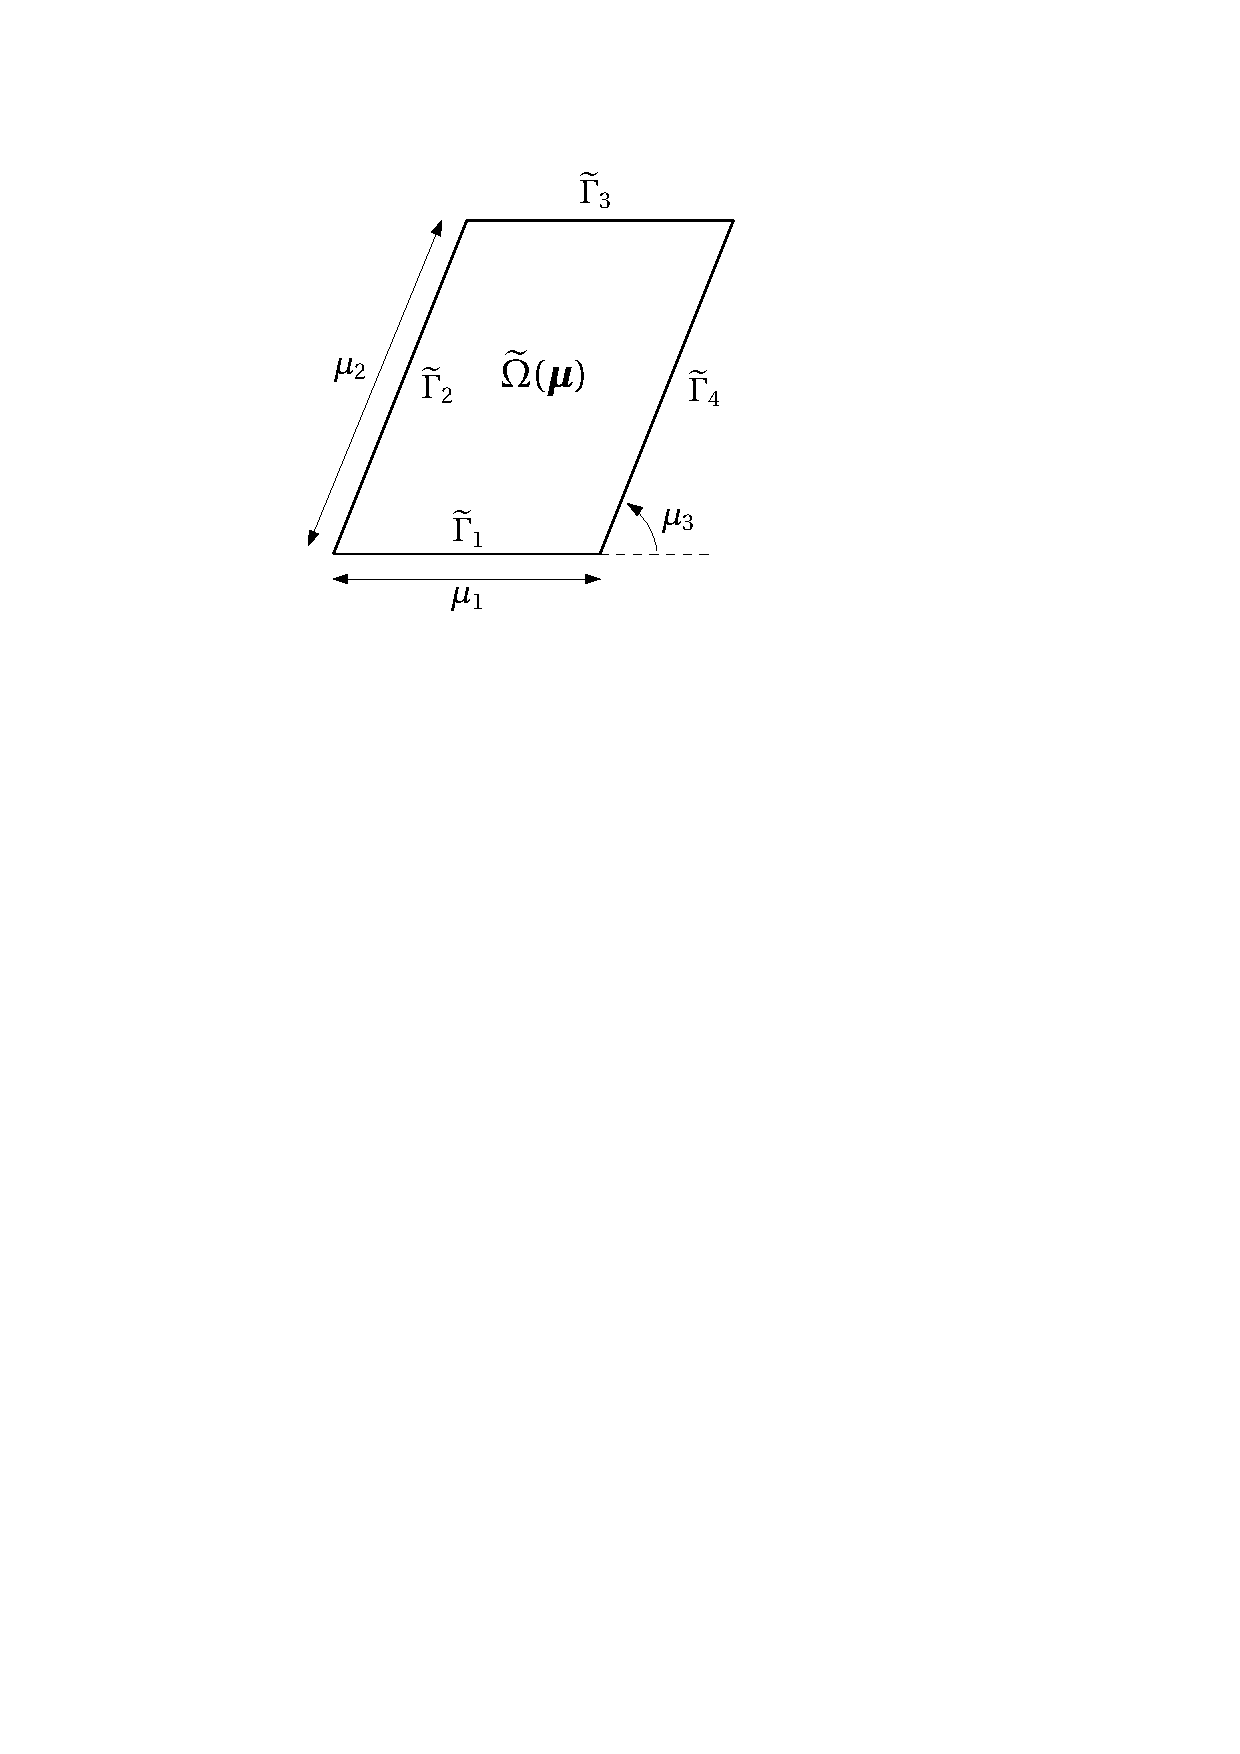
\includegraphics[scale = 0.6]{dc_domain}
			\end{minipage}
			\begin{minipage}{0.32\textwidth}
				\center
				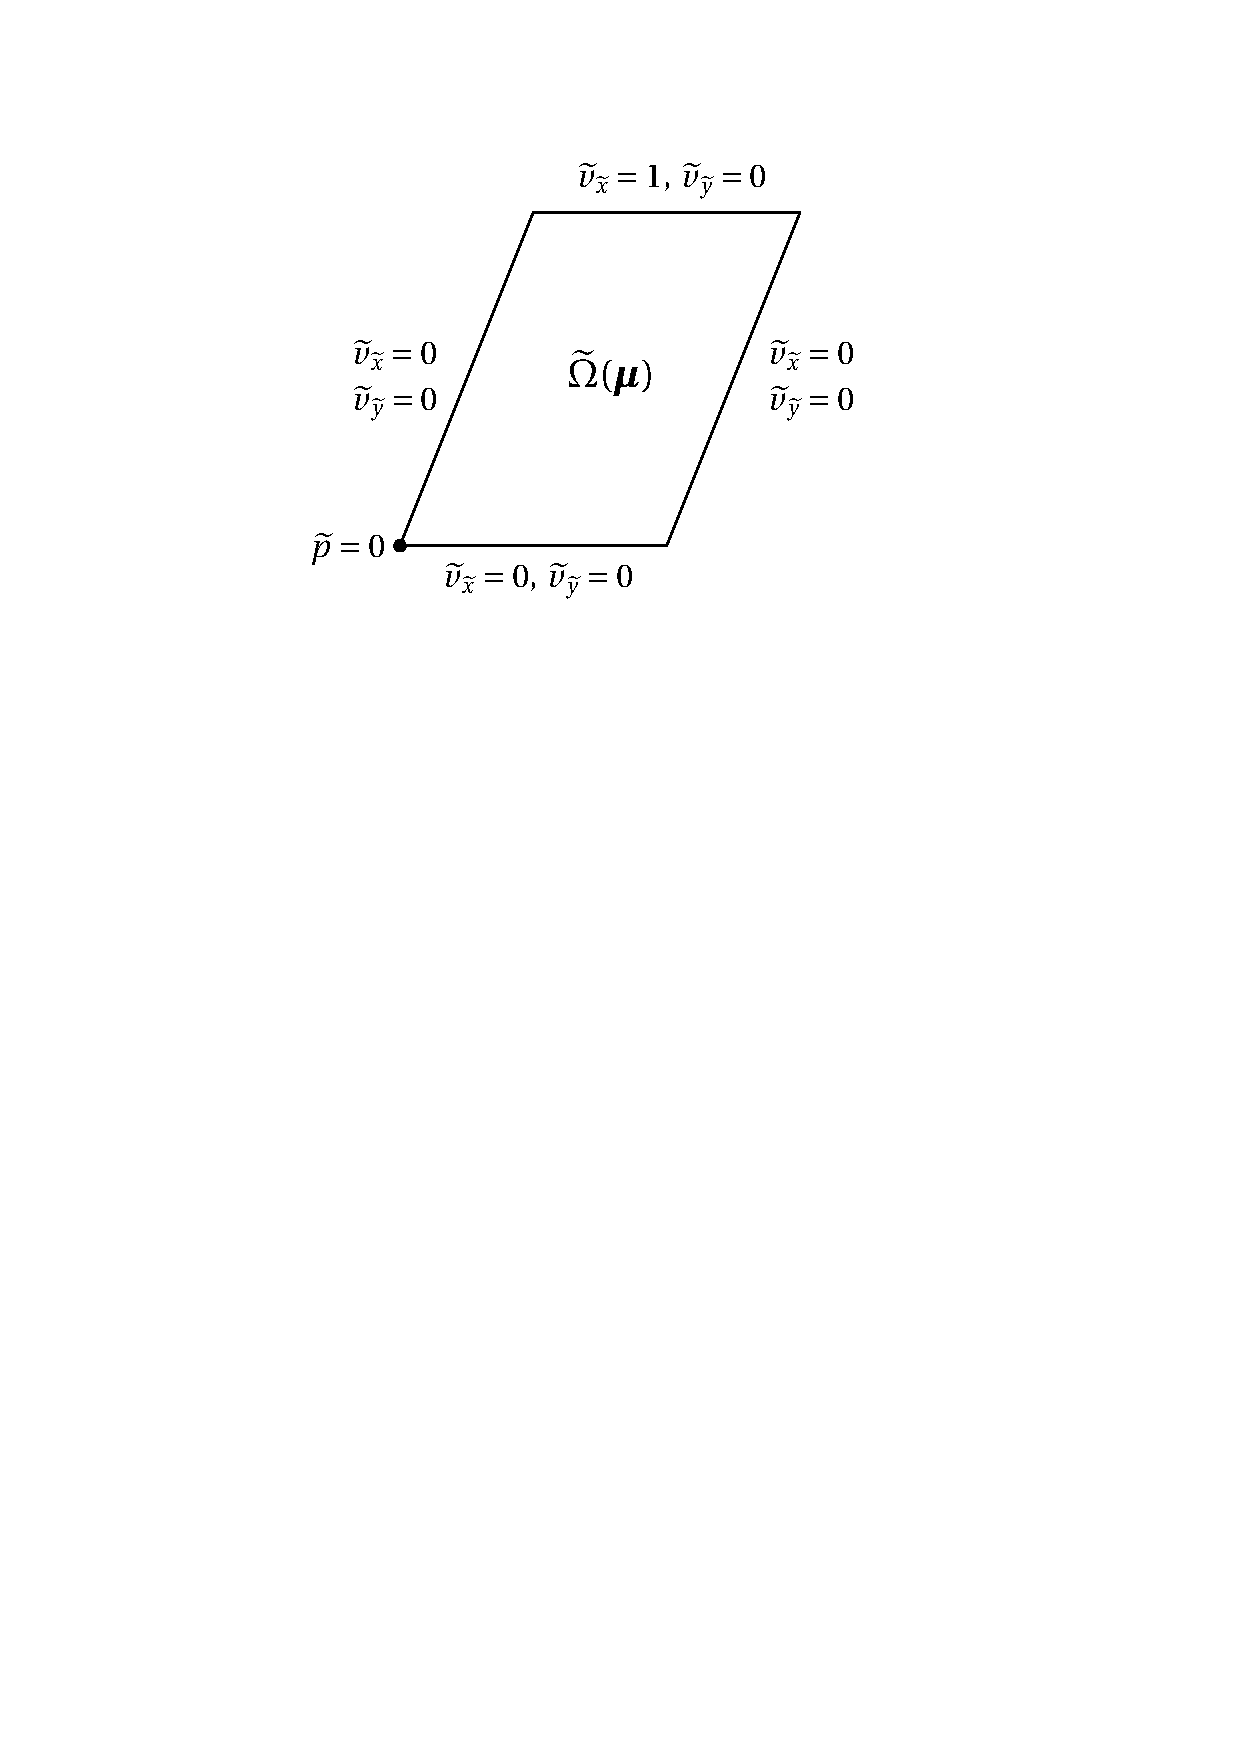
\includegraphics[scale = 0.6]{dc_domain_bc}
			\end{minipage}
			\begin{minipage}{0.32\textwidth}
				\center
				\vspace*{0.15cm}
				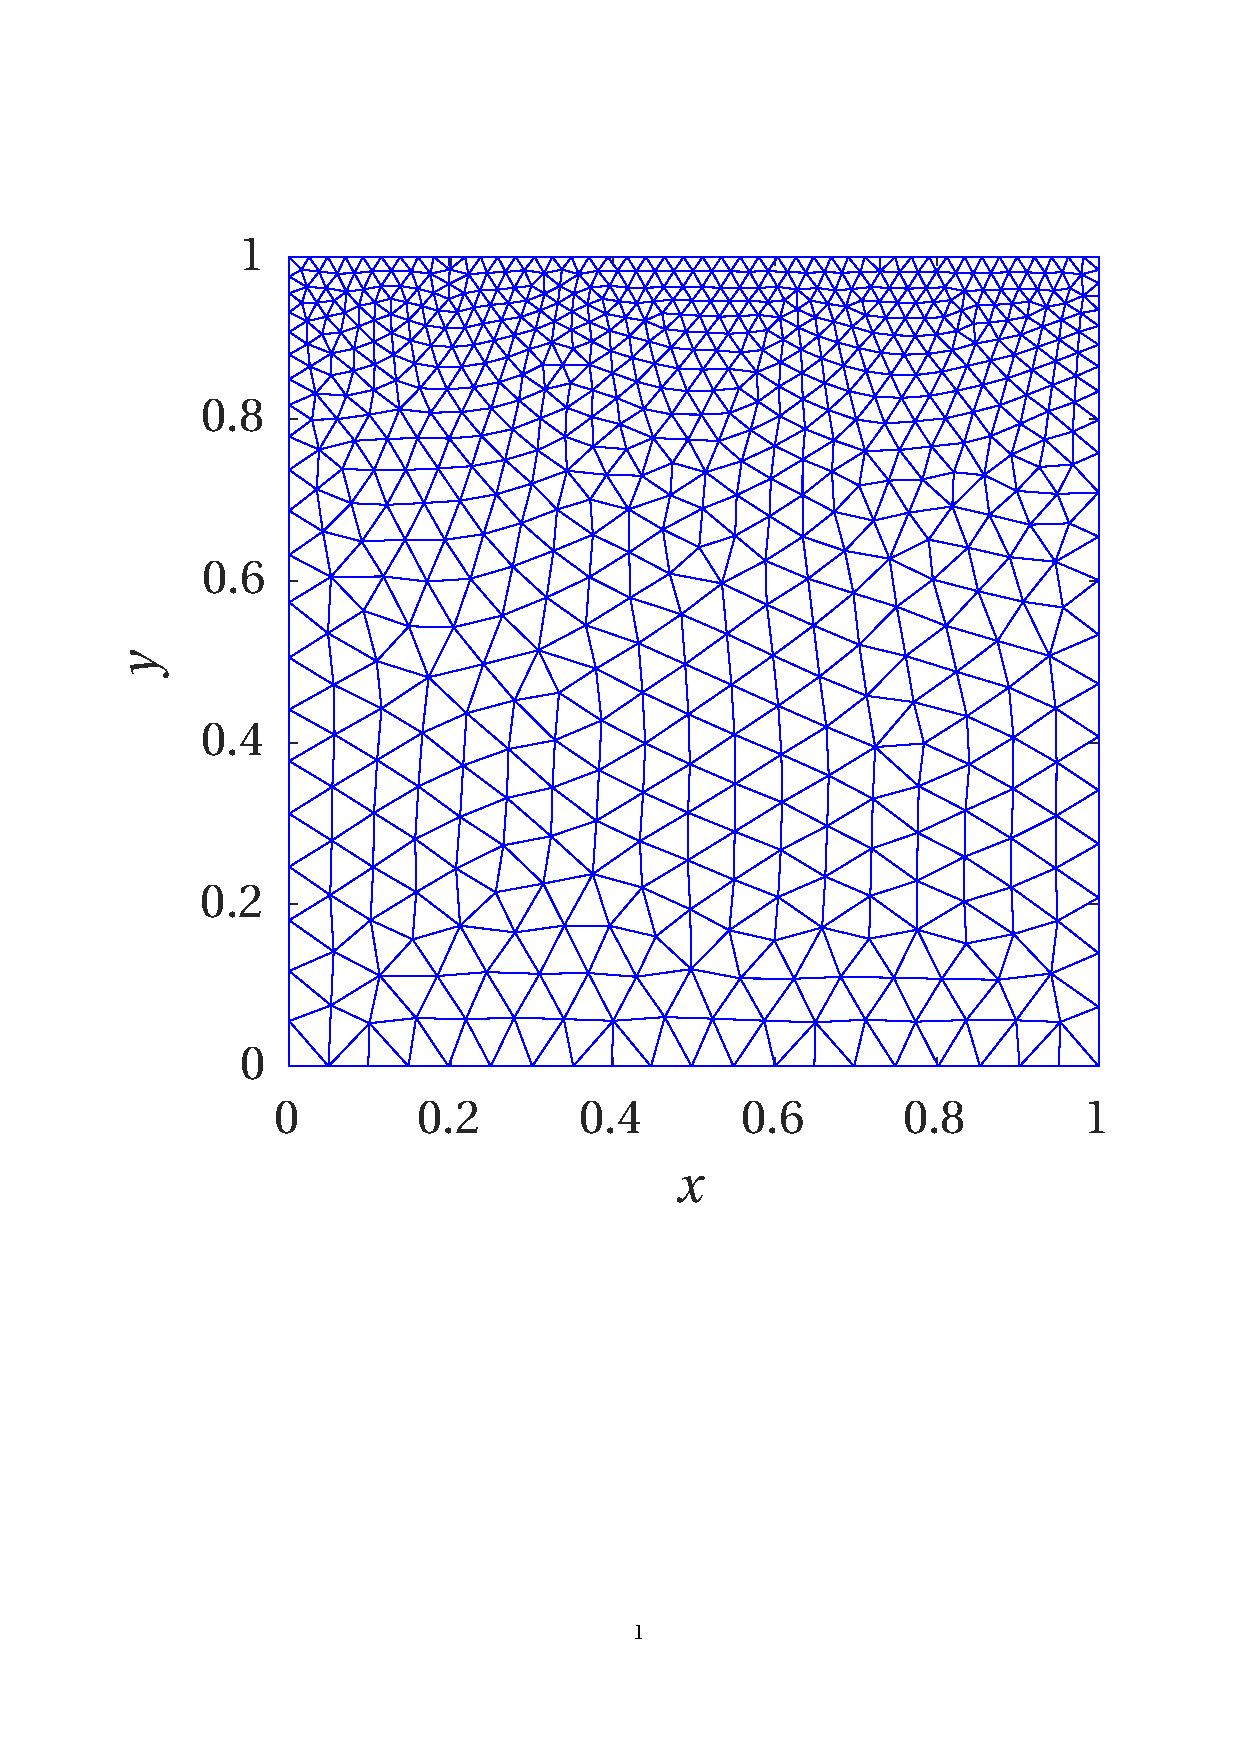
\includegraphics[scale = 0.275, trim = {2cm 9cm 1.5cm 3.5cm}, clip]{dc_mesh}
			\end{minipage}

			\vspace*{-0.1cm}
			
			\caption{Computational domain $\wt{\Omega}(\bg{\mu})$ (\emph{left}), enforced velocity at the boundaries (\emph{center}) and computational mesh $\Omega_h$ (\emph{right}) for the lid-driven cavity problem for the incompressible Navier-Stokes equations.}
			\label{fig:dc-domain}
			
			\center 
			\subfloat[$\bg{\mu} = \big( 1, \, \nicefrac{2}{\sqrt{3}}, \, \nicefrac{2 \pi}{3} \big)$]{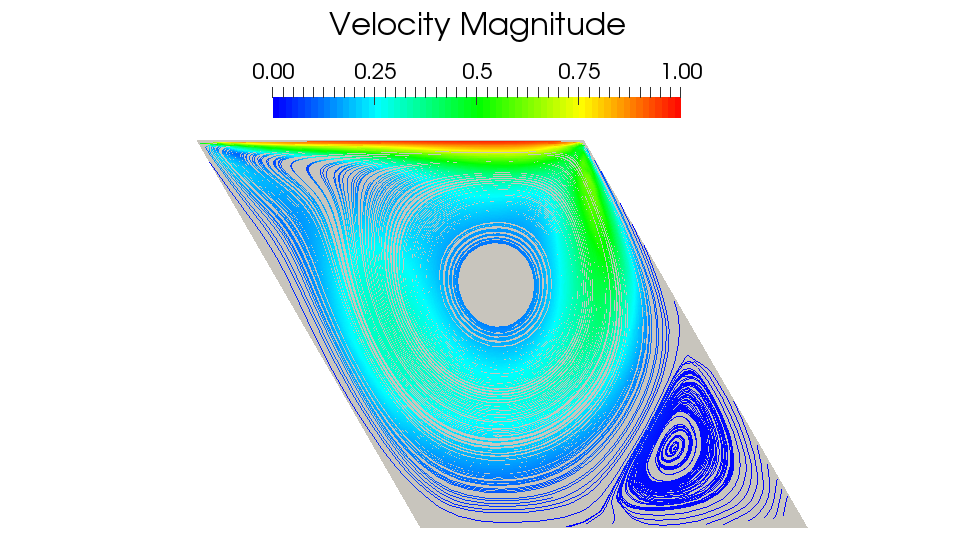
\includegraphics[scale = 0.25, trim = {6.5cm 0 5.5cm 0}, clip]{dc_400_vel_fem_solution_1}}
			\subfloat[$\bg{\mu} = \big( 1, \, 1, \, \nicefrac{\pi}{2} \big)$]{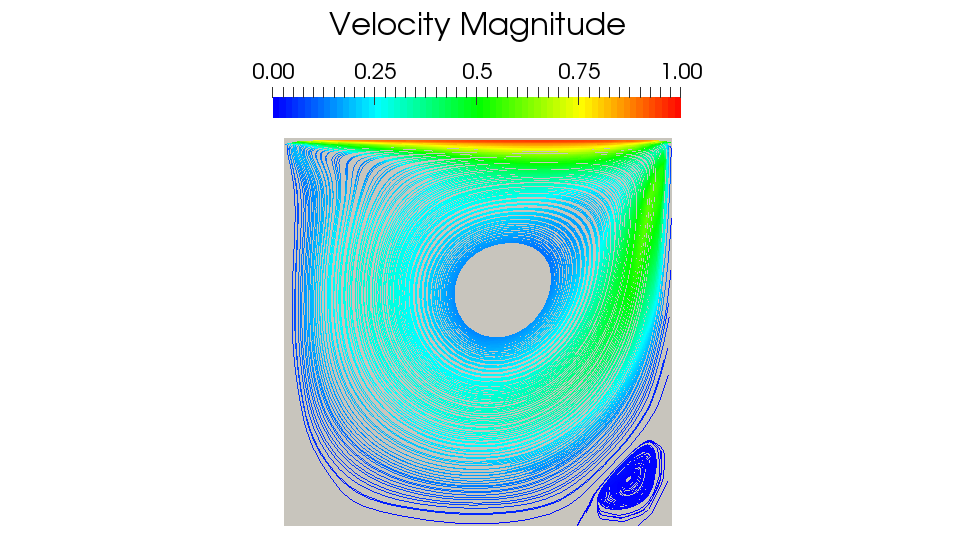
\includegraphics[scale = 0.25, trim = {7.5cm 0 7.5cm 0}, clip]{dc_400_vel_fem_solution_2}}
			\subfloat[$\bg{\mu} = \big( 1, \, \nicefrac{2}{\sqrt{3}}, \, \nicefrac{\pi}{3} \big)$]{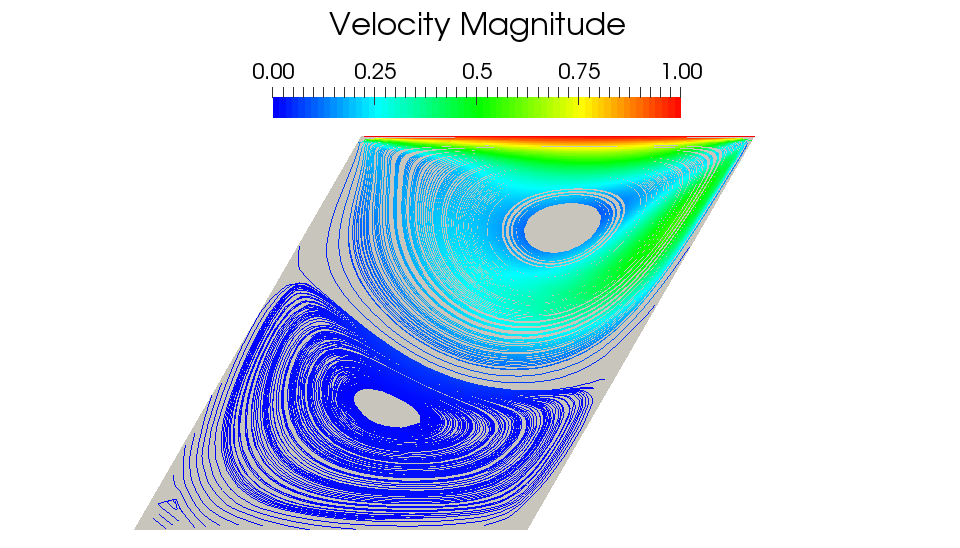
\includegraphics[scale = 0.25, trim = {4.8cm 0 5.5cm 0}, clip]{dc_400_vel_fem_solution_3}} \\
			\subfloat[$\bg{\mu} = \big( 1, \, \nicefrac{2}{\sqrt{3}}, \, \nicefrac{2 \pi}{3} \big)$]{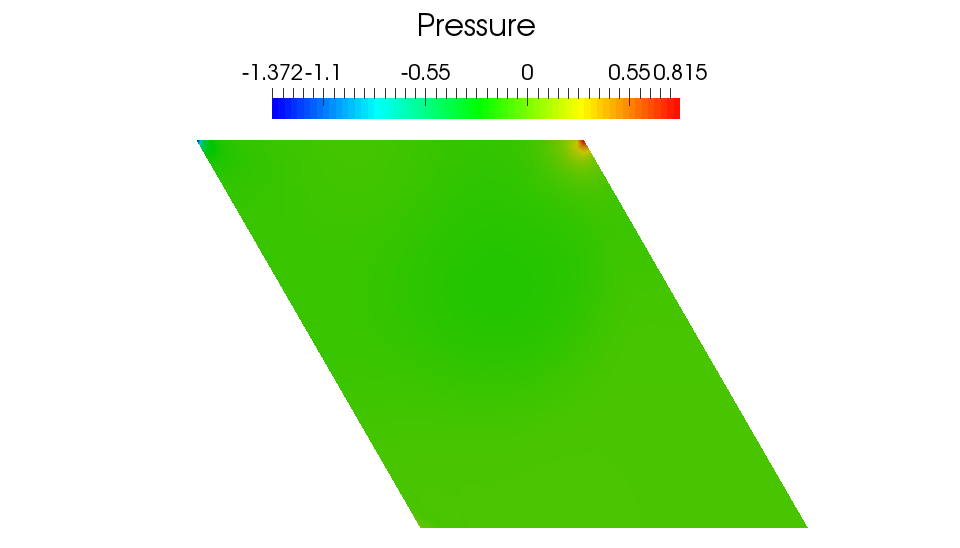
\includegraphics[scale = 0.25, trim = {6.5cm 0 5.5cm 0}, clip]{dc_400_p_fem_solution_1}}
			\subfloat[$\bg{\mu} = \big( 1, \, 1, \, \nicefrac{\pi}{2} \big)$]{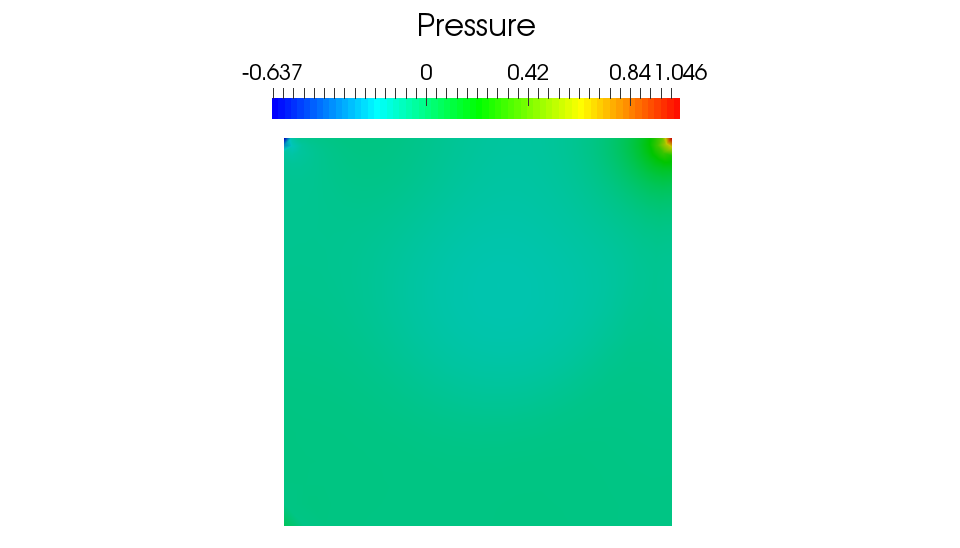
\includegraphics[scale = 0.25, trim = {7.5cm 0 7.5cm 0}, clip]{dc_400_p_fem_solution_2}}
			\subfloat[$\bg{\mu} = \big( 1, \, \nicefrac{2}{\sqrt{3}}, \, \nicefrac{\pi}{3} \big)$]{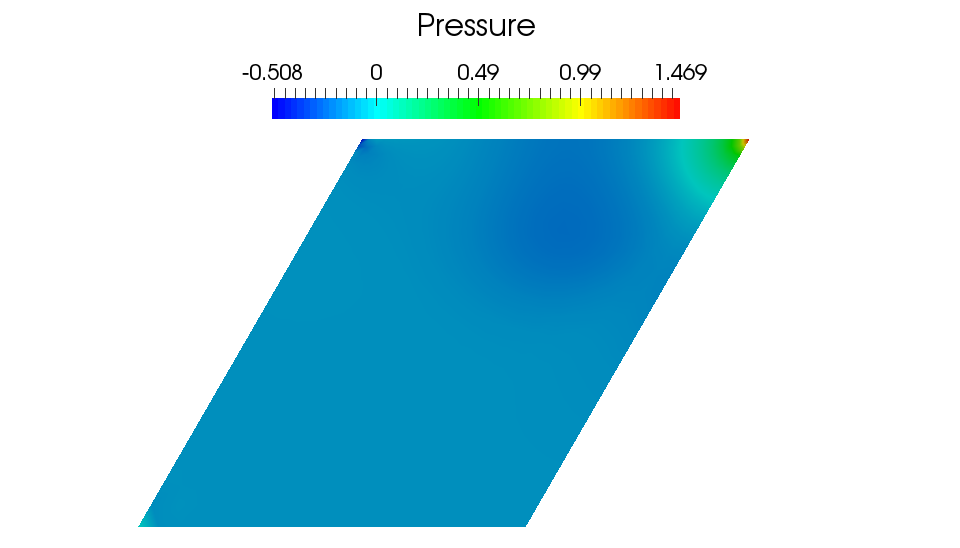
\includegraphics[scale = 0.25, trim = {5cm 0 5.5cm 0}, clip]{dc_400_p_fem_solution_3}}
					
			\caption{Velocity streamlines (\emph{top}) and pressure distribution (\emph{bottom}) for the lid-driven cavity problem, computed through the FE method. Three different parameter values are considered; for all configurations, the Reynold's number is $400$.}
			\label{fig:dc-solutions-different-domains}
		\end{figure}

		\clearpage

		For the Navier-Stokes equations, a suitable choice of the FE spaces is crucial to fulfill the well-known \emph{inf-sup} stability condition \cite{Ran99}. A common and effective choice consists in using quadratic finite elements for the components of the velocity field and linear finite elements for the pressure, leading to the so-called $\mathbb{P}^2 - \mathbb{P}^1$ (or Taylor-Hood) FE discretization \cite{Per02}. Figure \ref{fig:dc-solutions-different-domains} shows the velocity streamlines (\emph{top}) and the pressure distribution (\emph{bottom}) obtained through the resulting FE method for, from the left to the right, $\bg{\mu} = \big( 1, \, \nicefrac{2}{\sqrt{3}}, \, \nicefrac{2 \pi}{3} \big)$, $\bg{\mu} = \big( 1, \, 1, \, \nicefrac{\pi}{2} \big)$ or $\bg{\mu} = \big( 1, \, \nicefrac{2}{\sqrt{3}}, \, \nicefrac{\pi}{6} \big)$. Observe how the moving lid induces a large velocity gradient close to the top boundary, while it only slightly affects the fluid in the lower part of the cavity. In turn, this gives rise to two vortices, whose extent highly depends on the shape of the domain, or, equivalently, $\bg{\mu}$. Conversely, the pressure field does not undergo noticeable alterations across the parameter space. For all the configurations, a low-pressure region takes place at the upper-left corner of the domain and in the center of the major vortex (although it may be not clearly visible). Instead, the upper-right corner represents a stagnation point for the $\wt{x}$-velocity, and so therein the pressure assumes values larger than in the rest of the cavity \cite{Dho14}. All the results presented in Fig. \ref{fig:dc-solutions-different-domains} refer to a Reynold's number of $400$. For the specific problem at hand, the Reynold's number reads:
		\begin{linenomath}\begin{equation*}
			\vspace*{-0.1cm}
			Re = \dfrac{\max \big\lbrace \mu_1, \, \mu_2 \big\rbrace}{\nu(\bg{\mu})} \, .
		\end{equation*}\end{linenomath}
		In our analyses, $\nu(\bg{\mu})$ is adapted as the geometry varies so that the Reynold's number is either $200$ or $400$. 

		Regarding the reduced order modeling of the parametrized problem of interest, we slightly distance ourselves from the general workflow depicted in Sections \ref{section:Projection-based reduced basis method} and \ref{section:A non-intrusive RB method using neural networks}. Indeed, for the Navier-Stokes equations it is convenient to construct two separate reduced spaces \cite{Bal14, Chen17, QMN15}: $X_{\texttt{rb}}$, of dimension $L_{\bg{v}}$, for the velocity field and $Q_{\texttt{rb}}$, of dimension $L_p$, for the pressure distribution, respectively represented by the matrices 
		\begin{linenomath}\begin{equation*}
			\mathbb{V}_{\bg{v}} = \left[ \bg{\psi}_1^{\bg{v}} \, \big| \, \ldots \, \big| \, \bg{\psi}_{L_{\bg{v}}}^{\bg{v}} \right] \in \mathbb{R}^{N_h^{\bg{v}} \times L_{\bg{v}}} \hspace*{0.5cm} \text{and} \hspace*{0.5cm} \mathbb{V}_p = \left[ \bg{\psi}_1^p \, \big| \, \ldots \, \big| \, \bg{\psi}_{L_p}^p \right] \in \mathbb{R}^{N_h^p \times L_p} \, ,
		\end{equation*}\end{linenomath} 
		with $N_h^{\bg{v}}$ (respectively, $N_h^p$) the dimension of the FE velocity (resp., pressure) space. Although the underpinning finite element solver has been designed to fulfill the inf-sup condition, thus ensuring the stability of the scheme, when dealing with incompressible flows this property may not be automatically inherited by the POD-Galerkin reduced order solver. As a result, it may show severe instabilities \cite{Bur06}. Indeed, one has to carefully choose the reduced velocity space $X_{\texttt{rb}}$ so to meet an equivalent of the inf-sup condition at the reduced level. To this end, in our simulations we resort to a \emph{supremizer enrichment} of $X_{\texttt{rb}}$, as proposed in \cite{Bal14}. At each pressure snapshot $\mathbf{p}_h \big( \bg{\mu}^{(n)} \big) \in \mathbb{R}^{N_h^p}$, $n = 1, \, \ldots \, , N$, we associate the \emph{supremizer solution} $\mathbf{s}_h \big( \bg{\mu}^{(n)} \big) \in \mathbb{R}^{N_h^{\bg{v}}}$, defined as the solution to a linear system of the form
		\vspace*{-0.1cm}
		\begin{linenomath}\begin{equation*}
			\mathbb{A} \,\, \mathbf{s}_h \big( \bg{\mu}^{(n)} \big) = \mathbb{B} \big( \bg{\mu}^{(n)} \big) \, \mathbf{p}_h \big( \bg{\mu}^{(n)} \big) \, ,
			\vspace*{-0.1cm}
		\end{equation*}\end{linenomath}
		with $\mathbb{A} \in \mathbb{R}^{N_h^{\bg{v}} \times N_h^{\bg{v}}}$ and $\mathbb{B} \big( \bg{\mu}^{(n)} \big) \in \mathbb{R}^{N_h^{\bg{v}} \times N_h^p}$. Letting 
		\vspace*{-0.1cm}
		\begin{linenomath}\begin{equation*}
			\mathbb{V}_{\bg{s}} = \left[ \bg{\psi}_1^{\bg{s}} \, \big| \, \ldots \, \big| \, \bg{\psi}_{L_{\bg{s}}}^{\bg{s}} \right] \in \mathbb{R}^{N_h^{\bg{v}} \times L_{\bg{s}}} 
			\vspace*{-0.1cm}
		\end{equation*}\end{linenomath}
		be the POD basis of rank $L_{\bg{s}}$ extracted from the ensemble of snapshots $\big\lbrace \mathbf{s}_h \big( \bg{\mu}^{(1)} \big) , \, \ldots \, , \mathbf{s}_h \big( \bg{\mu}^{(N)} \big) \big\rbrace$, the POD-G approximation of the velocity field is then sought in the form
		\vspace*{-0.2cm}
		\begin{linenomath}\begin{equation*}
			\bar{\mathbf{v}}_L(\bg{\mu}) = \overline{\mathbb{V}}_{\bg{v}} \, \bar{\mathbf{v}}_{\texttt{rb}}(\bg{\mu}) = \sum_{i = 1}^{L_{\bg{v}}} v_{\texttt{rb}}^{(i)} \bg{\psi}_i^{\bg{v}} + \sum_{i = 1}^{L_{\bg{s}}} s_{\texttt{rb}}^{(i)} \bg{\psi}_i^{\bg{s}} \, ,
		\end{equation*}\end{linenomath} 
		where
		\begin{linenomath}\begin{equation*}
			\overline{\mathbb{V}}_{\bg{v}} = \left[ \mathbb{V}_{\bg{v}} ~ \mathbb{V}_{\bg{s}} \right] \in \mathbb{R}^{N_h^{\bg{v}} \times (L_{\bg{v}} + L_{\bg{s}})} \hspace*{0.5cm} \text{and} \hspace*{0.5cm} \bar{\mathbf{v}}_{\texttt{rb}}(\bg{\mu}) =
			\begin{bmatrix}
			\hspace*{-0.15cm}
			\begin{array}{c}
				\mathbf{v}_{\texttt{rb}}(\bg{\mu}) \\
				\mathbf{s}_{\texttt{rb}}(\bg{\mu})
			\end{array} 
			\hspace*{-0.15cm}
			\end{bmatrix} 
			\in \mathbb{R}^{L_{\bg{v}} + L_{\bg{s}}} \, .
		\end{equation*}\end{linenomath}
		In \cite{Bal14}, several numerical evidences suggest that a proper value for $L_{\bg{s}}$ should lay in between $L_p / 2$ and $L_p$. In our simulations, we set $L_{\bg{s}} = L_p = L_{\bg{v}}$, leading to a stable reduced (nonlinear) system in $L = 3 \, L_{\bg{v}}$ unknowns.

		Concerning the POD-NN procedure, for any $\bg{\mu} \in \mathcal{P}$, reduced order discretizations $\mathbf{v}_{L_{\bg{v}}}^{\texttt{NN}}(\bg{\mu})$ and $\mathbf{p}_{L_p}^{\texttt{NN}}(\bg{\mu})$ of $\bg{v}(\bg{\mu})$ and $p(\bg{\mu})$, respectively, are sought in the form
		\begin{linenomath}\begin{equation*}
			\mathbf{v}_{L_{\bg{v}}}^{\texttt{NN}}(\bg{\mu}) = \mathbb{V}_{\bg{v}} \, \mathbf{v}_{\texttt{rb}}^{\texttt{NN}}(\bg{\mu}) \hspace*{0.5cm} \text{and} \hspace*{0.5cm} \mathbf{p}_{L_p}^{\texttt{NN}}(\bg{\mu}) = \mathbb{V}_{p} \, \mathbf{p}_{\texttt{rb}}^{\texttt{NN}}(\bg{\mu}) \, .
		\end{equation*}\end{linenomath}
		Here, $\mathbf{v}_{\texttt{rb}}^{\texttt{NN}}(\bg{\mu})$ and $\mathbf{p}_{\texttt{rb}}^{\texttt{NN}}(\bg{\mu})$ denote the output vectors provided by two \emph{distinct} multi-layer perceptrons, respectively trained with the ensemble of input-output patterns
		\begin{linenomath}\begin{equation*}
			\big\lbrace \bg{\mu}^{(i)}, \, \mathbb{V}_{\bg{v}}^T \, \mathbf{v}_h \big( \bg{\mu}^{(i)} \big) \big\rbrace_{1 \leq i \leq N_{tr}} \hspace*{0.5cm} \text{and} \hspace*{0.5cm} \big\lbrace \bg{\mu}^{(i)}, \, \mathbb{V}_{p}^T \, \mathbf{p}_h \big( \bg{\mu}^{(i)} \big) \big\rbrace_{1 \leq i \leq N_{tr}} \, .
		\end{equation*}\end{linenomath}
		At this regard, let us point out two important remarks.
		\begin{enumerate}[label=(\roman*)]
			\item The supremizer solutions are not involved (either directly or indirectly) in the POD-NN framework. Indeed, they ensure the overall stability of the POD-G procedure, but they do not improve the accuracy of the method, and so they can be disregarded whenever stability is not an issue.
			\item The routine outlined in Section \ref{section:A non-intrusive RB method using neural networks}, aiming at finding an optimal network configuration, is applied \emph{separately} to the perceptrons designated to predict the velocity field and to the perceptrons required to approximate the pressure distribution. As a result, once the offline phase of the POD-NN method is completed, we end up with two different networks, equipped with $H_1^{\bg{v}} = H_2^{\bg{v}}$ and $H_1^p = H_2^p$ computing units per hidden layer, respectively.  
		\end{enumerate}

		\begin{figure}[t!]
			\center
			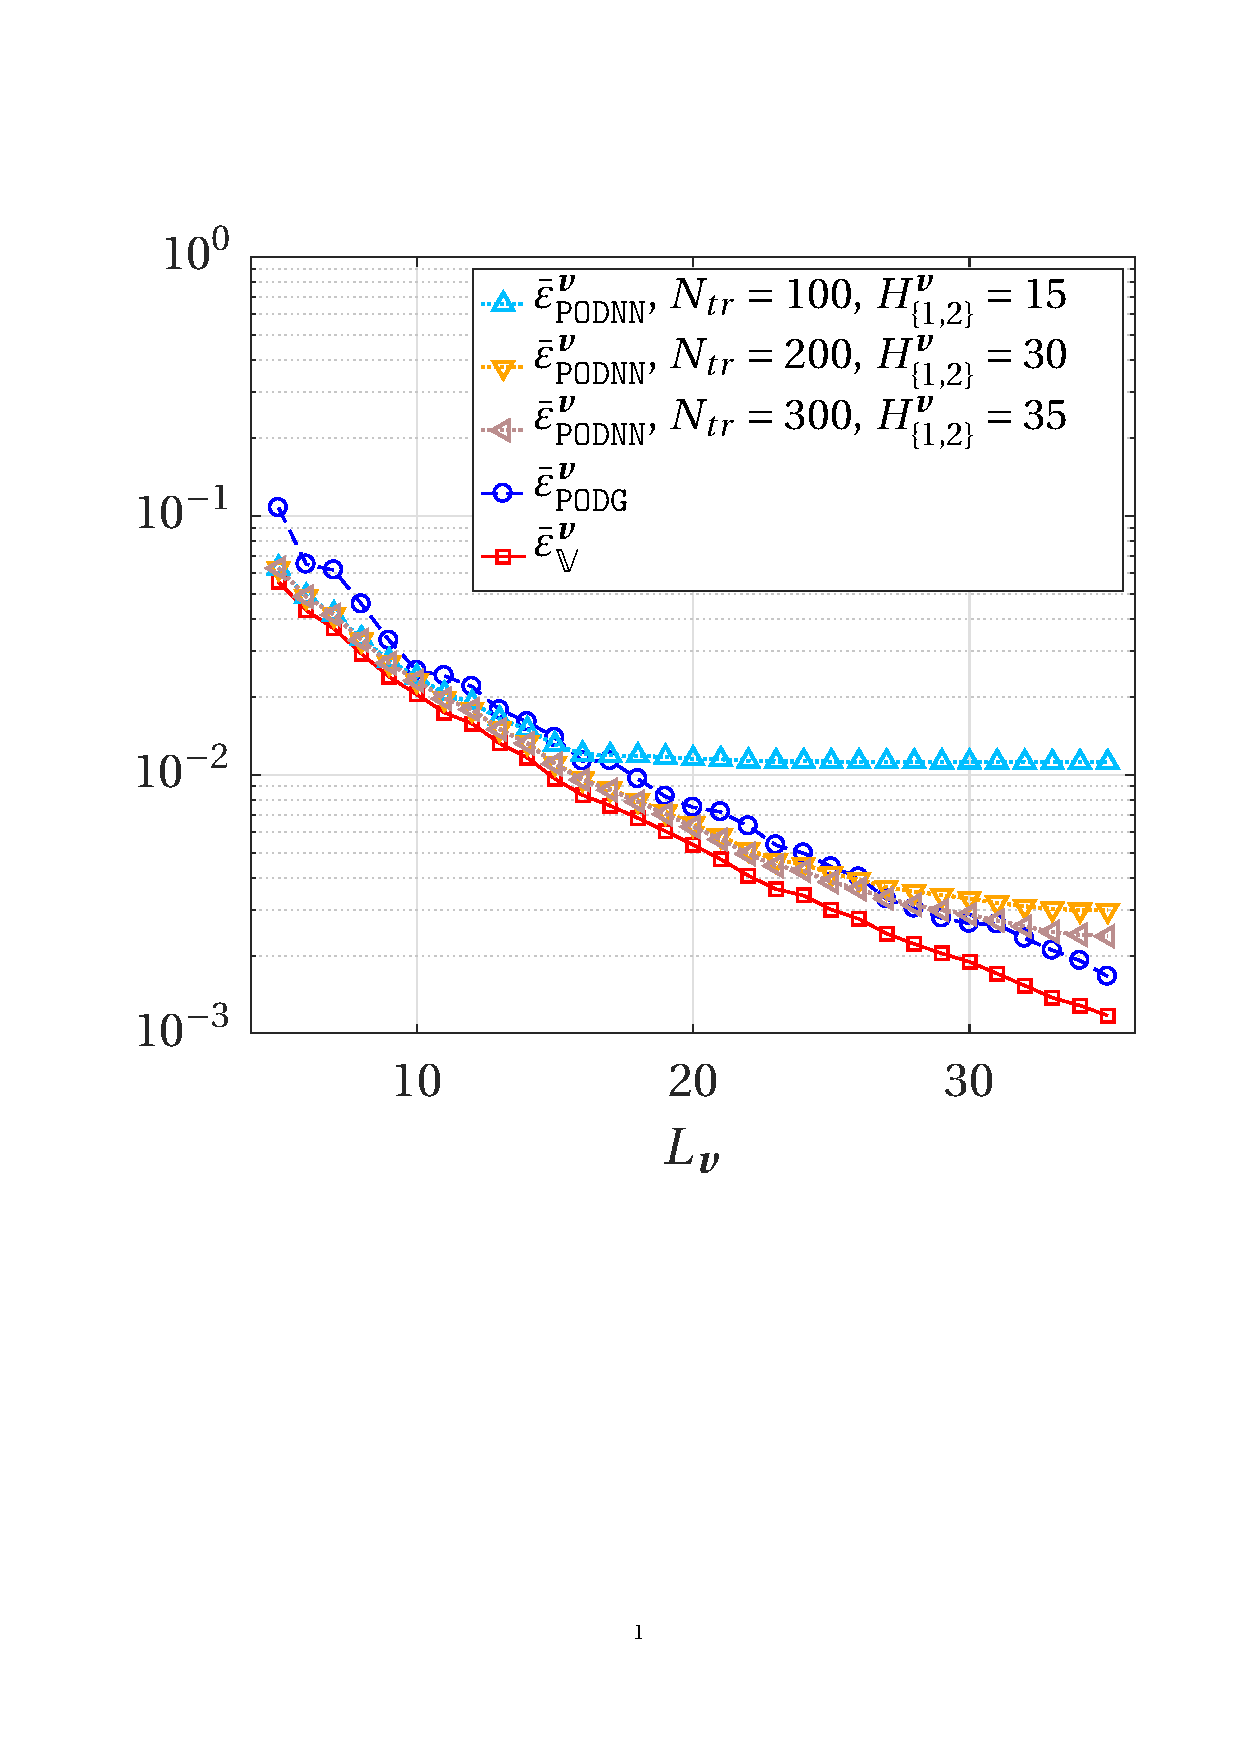
\includegraphics[scale = 0.37, trim = {2cm 9cm 1.5cm 3.5cm}, clip]{dc_200_vel_error_vs_rank}
			\hspace*{1cm}
			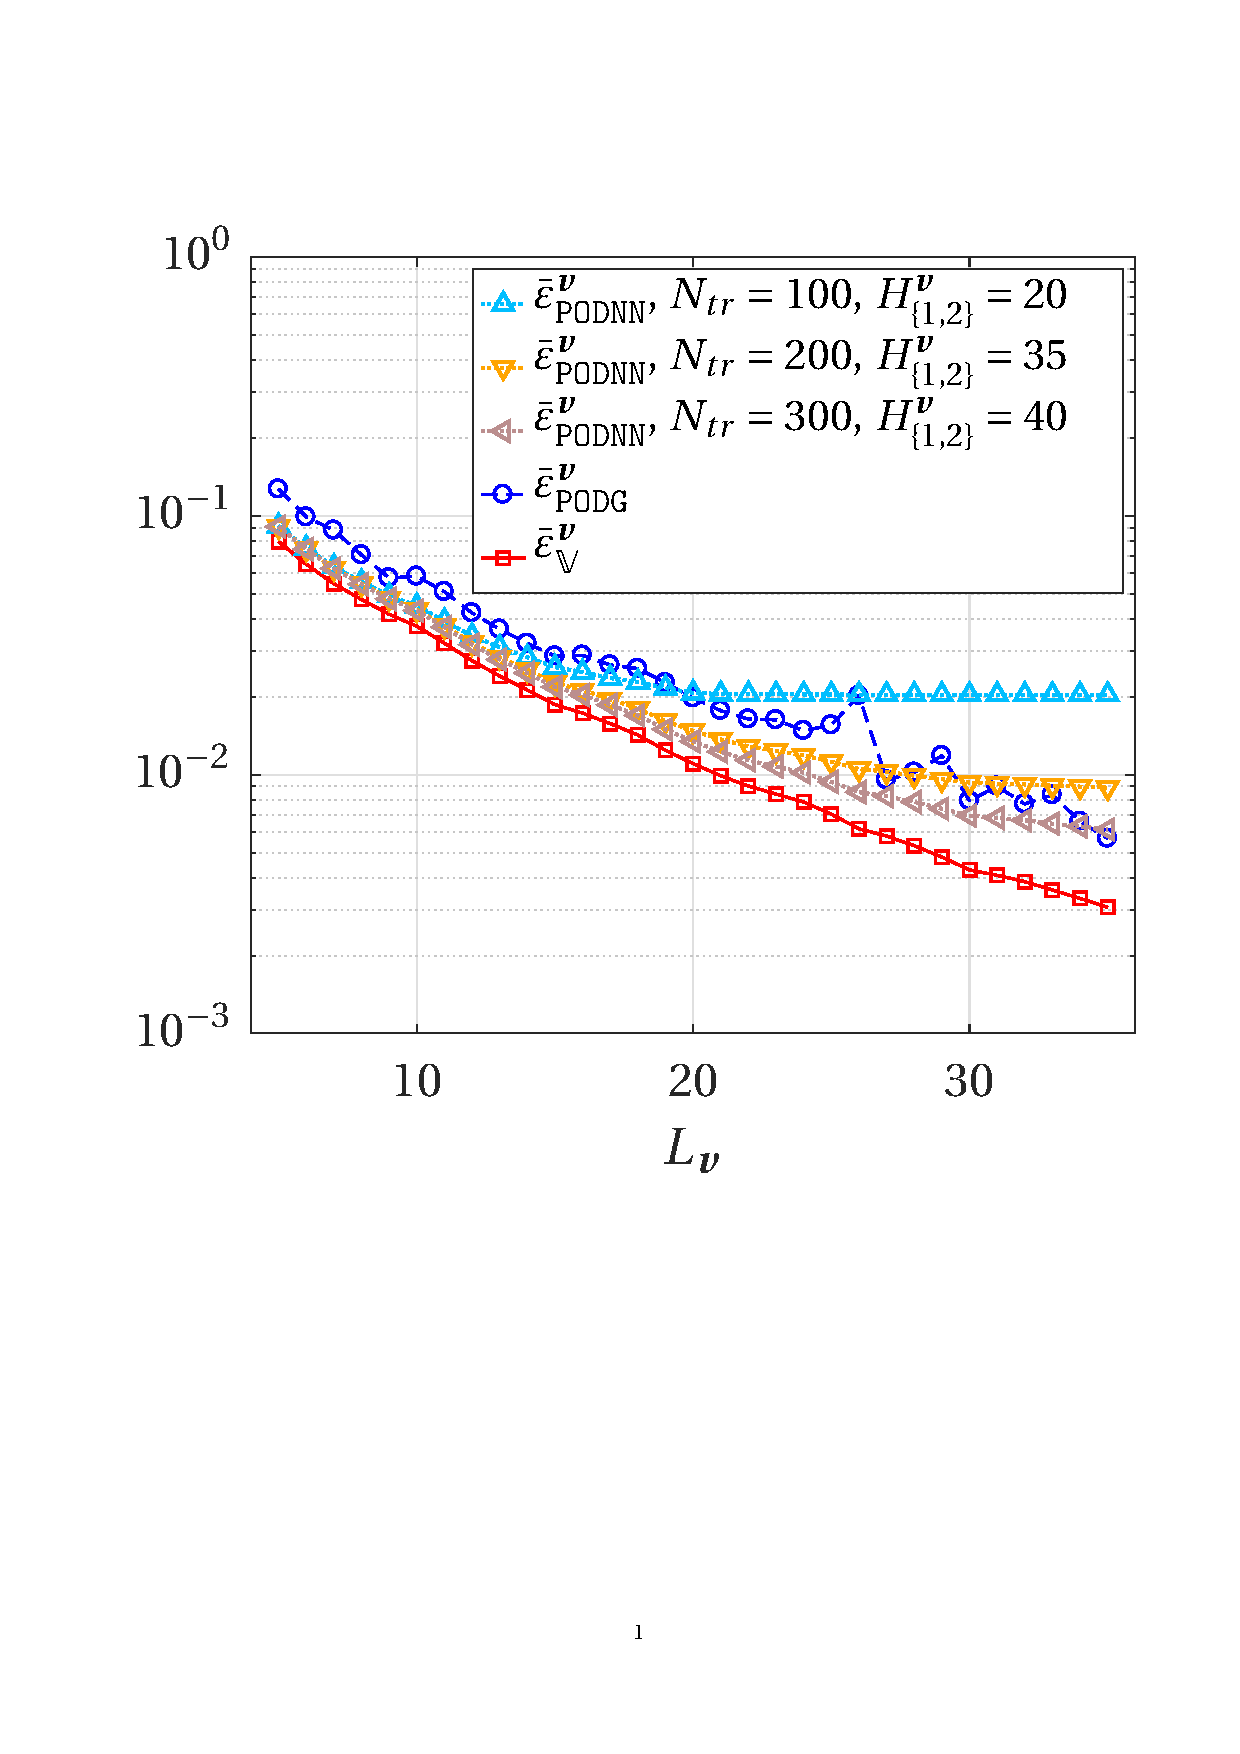
\includegraphics[scale = 0.37, trim = {2cm 9cm 1.5cm 3.5cm}, clip]{dc_400_vel_error_vs_rank} \\
			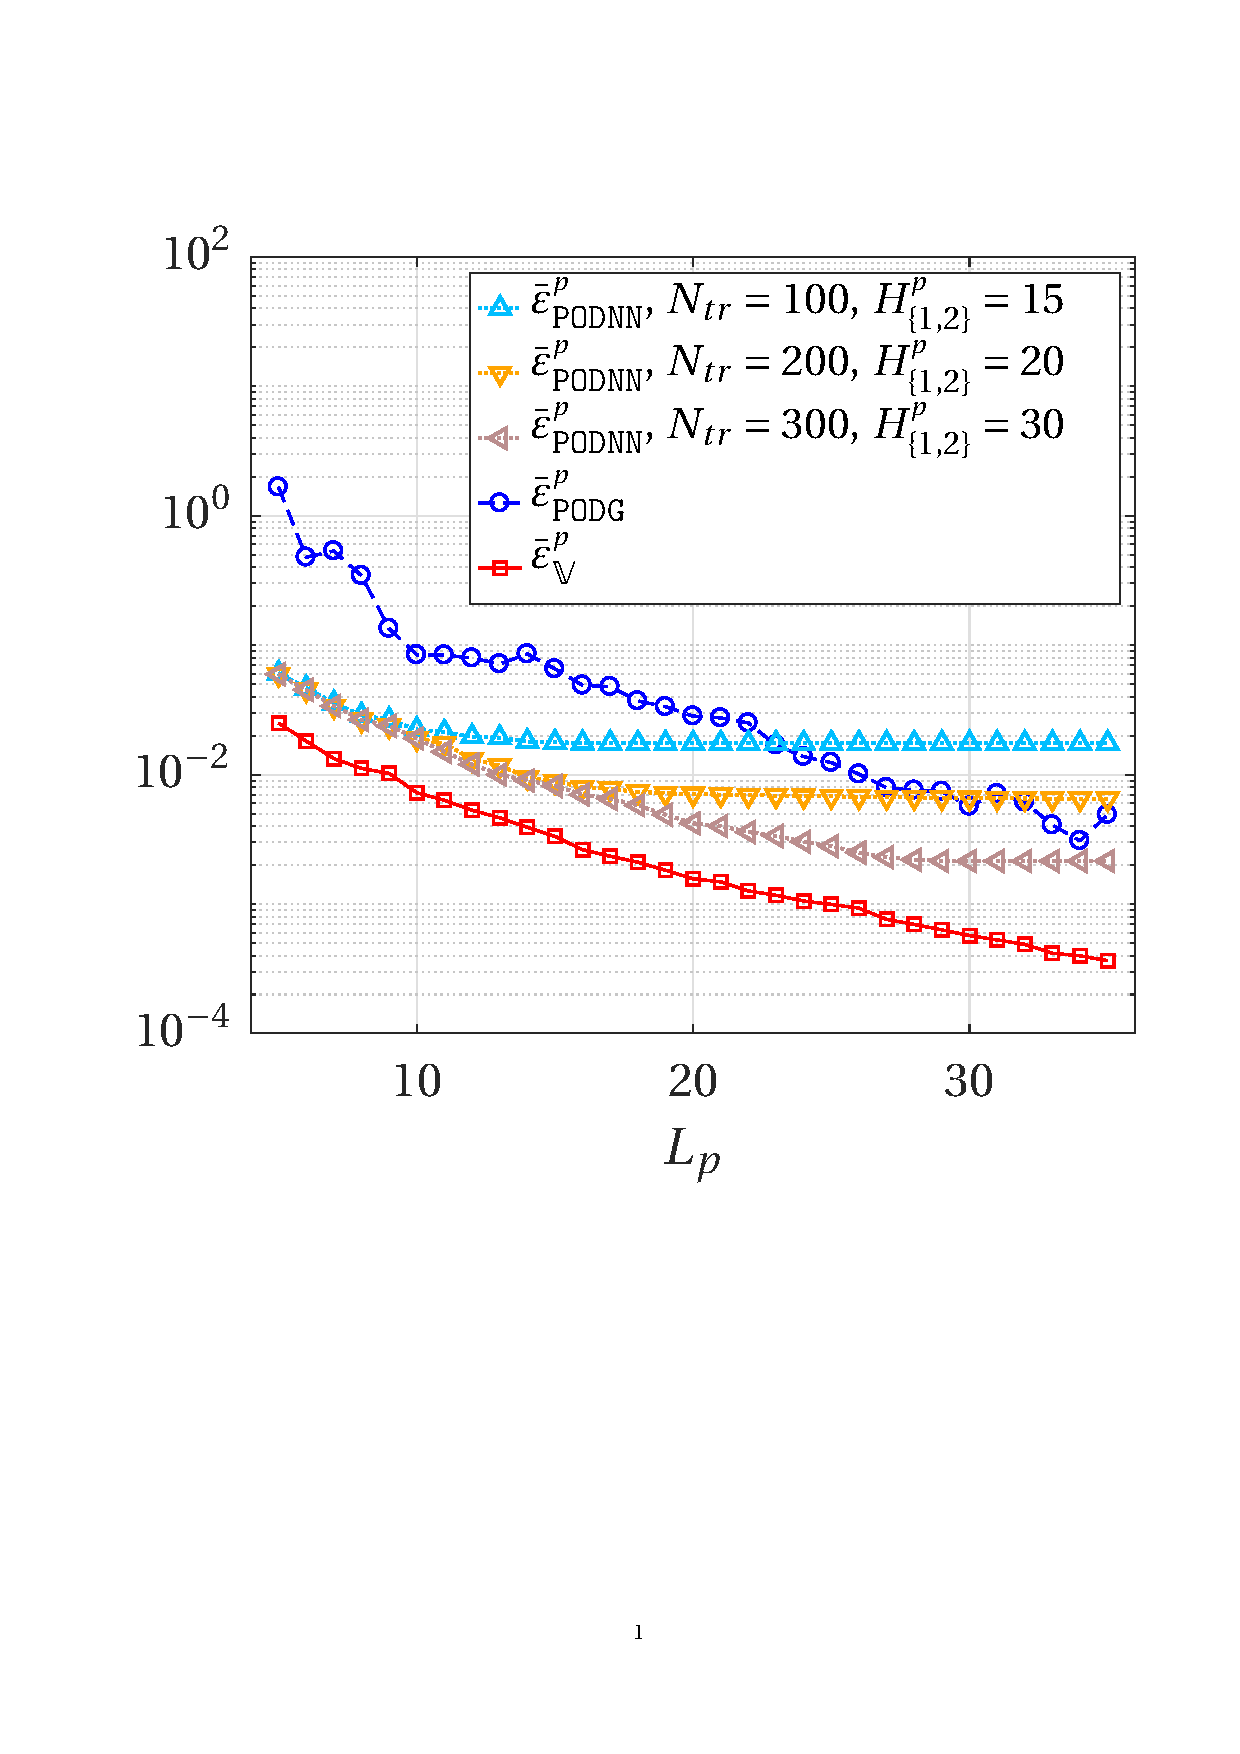
\includegraphics[scale = 0.37, trim = {2cm 9cm 1.5cm 3.5cm}, clip]{dc_200_p_error_vs_rank}
			\hspace*{1cm}
			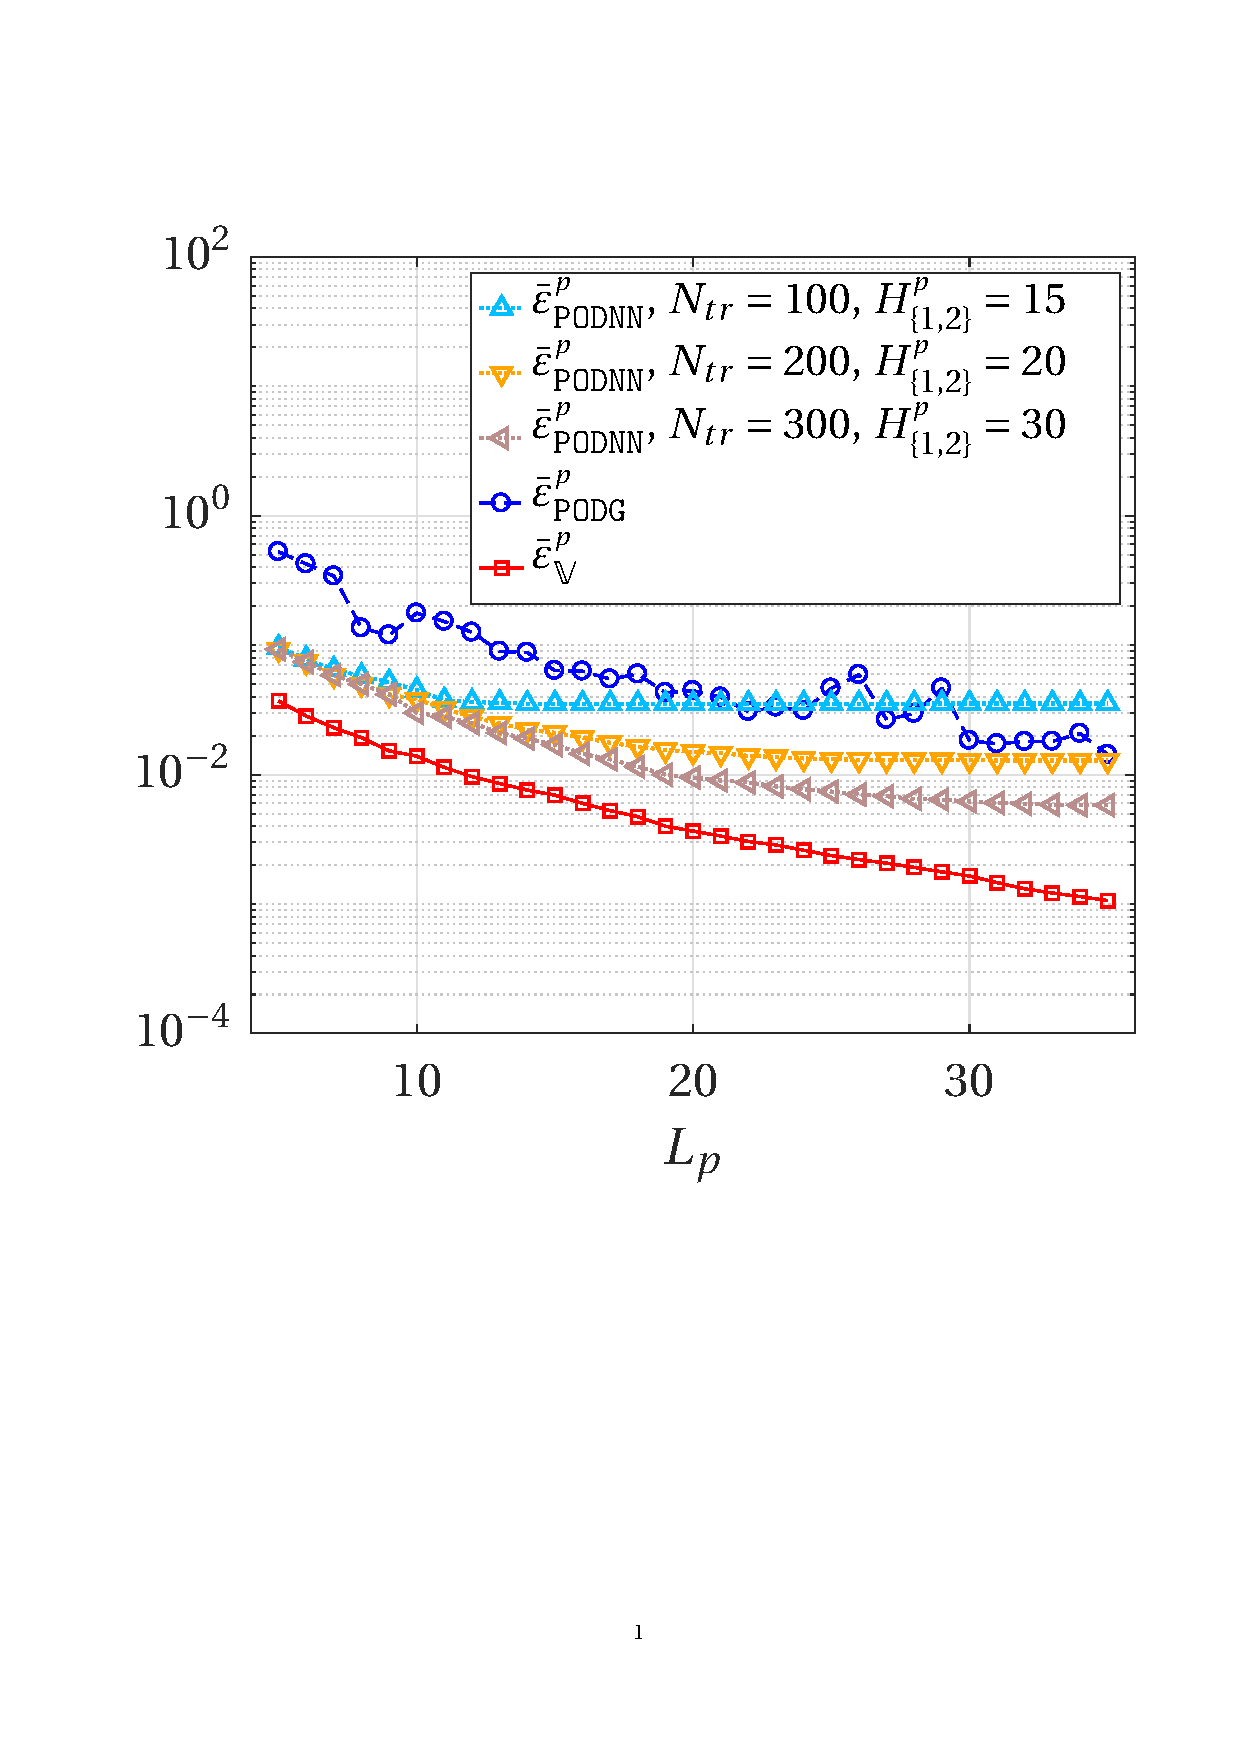
\includegraphics[scale = 0.37, trim = {2cm 9cm 1.5cm 3.5cm}, clip]{dc_400_p_error_vs_rank}
			
			\vspace*{-0.3cm}

			\caption{Velocity (\textcolor{deepgreen}{\emph{top}}) and pressure (\textcolor{deepgreen}{\emph{bottom}}) error analysis for the POD-G and POD-NN methods applied to the lid-driven cavity problem with $Re = 200$ (\textcolor{deepgreen}{\emph{left}}) and $Re = 400$ (\textcolor{deepgreen}{\emph{right}}).}
			\label{fig:dc-error-vs-rank}
		\end{figure}

		\begin{figure}[h!]
			\center
			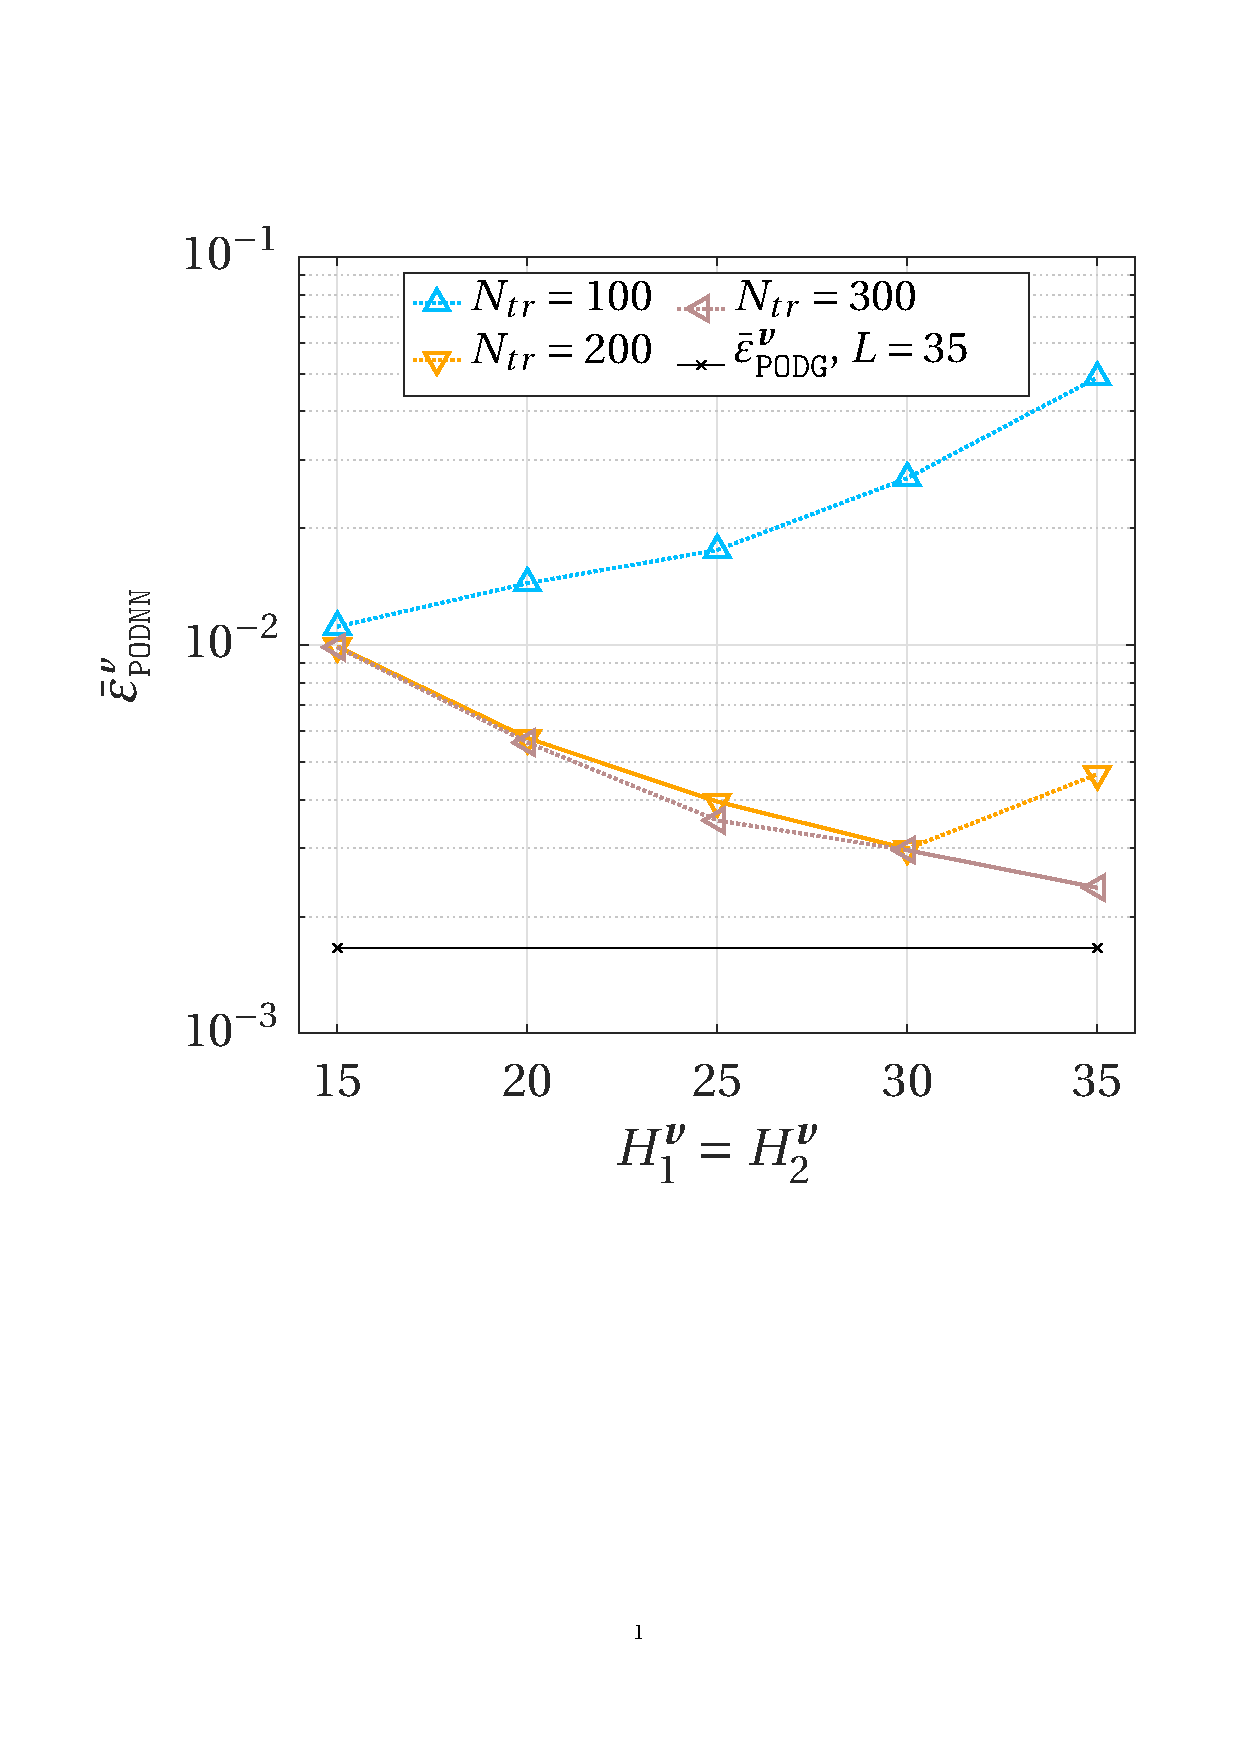
\includegraphics[scale = 0.37, trim = {1cm 9cm 1.5cm 3.5cm}, clip]{dc_200_vel_nn_convergence}
			\hspace*{1cm}
			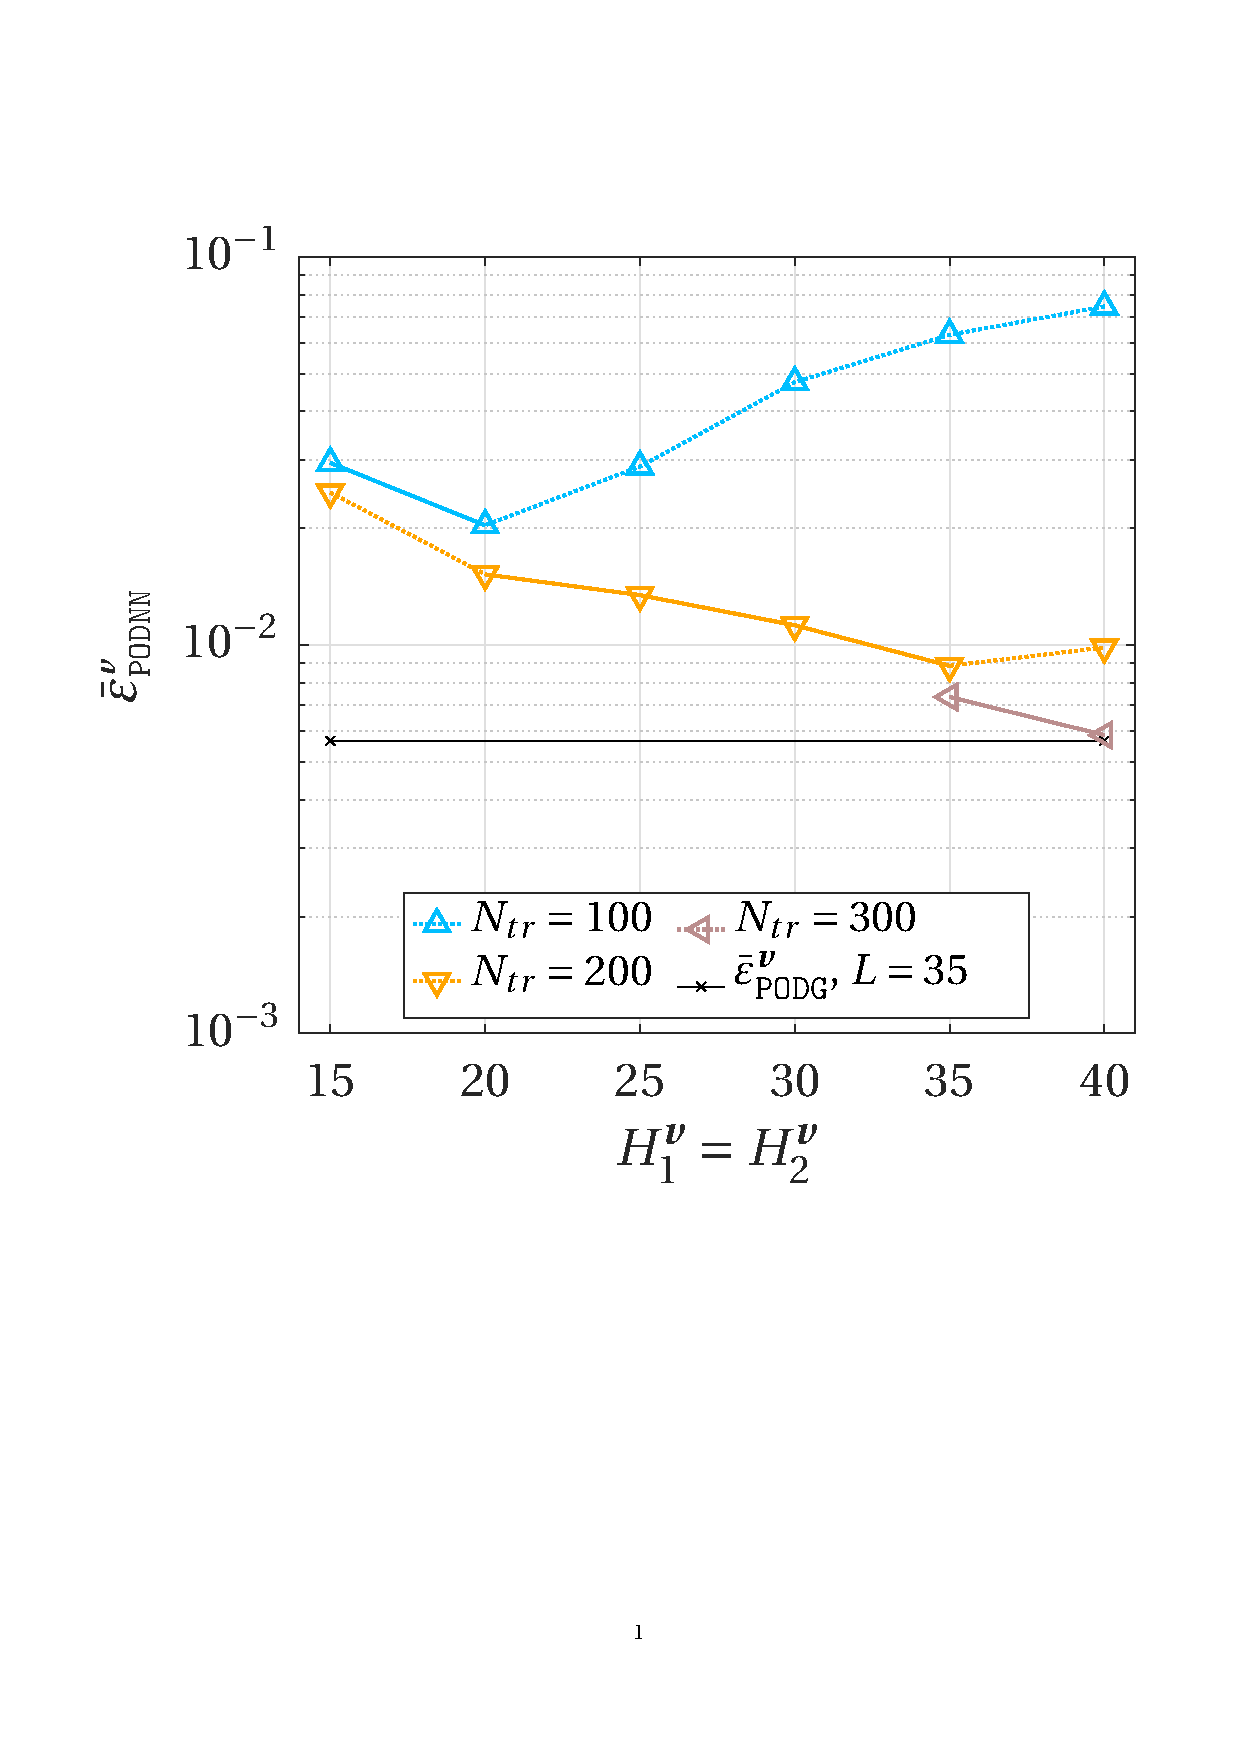
\includegraphics[scale = 0.37, trim = {1cm 9cm 1.5cm 3.5cm}, clip]{dc_400_vel_nn_convergence} \\
			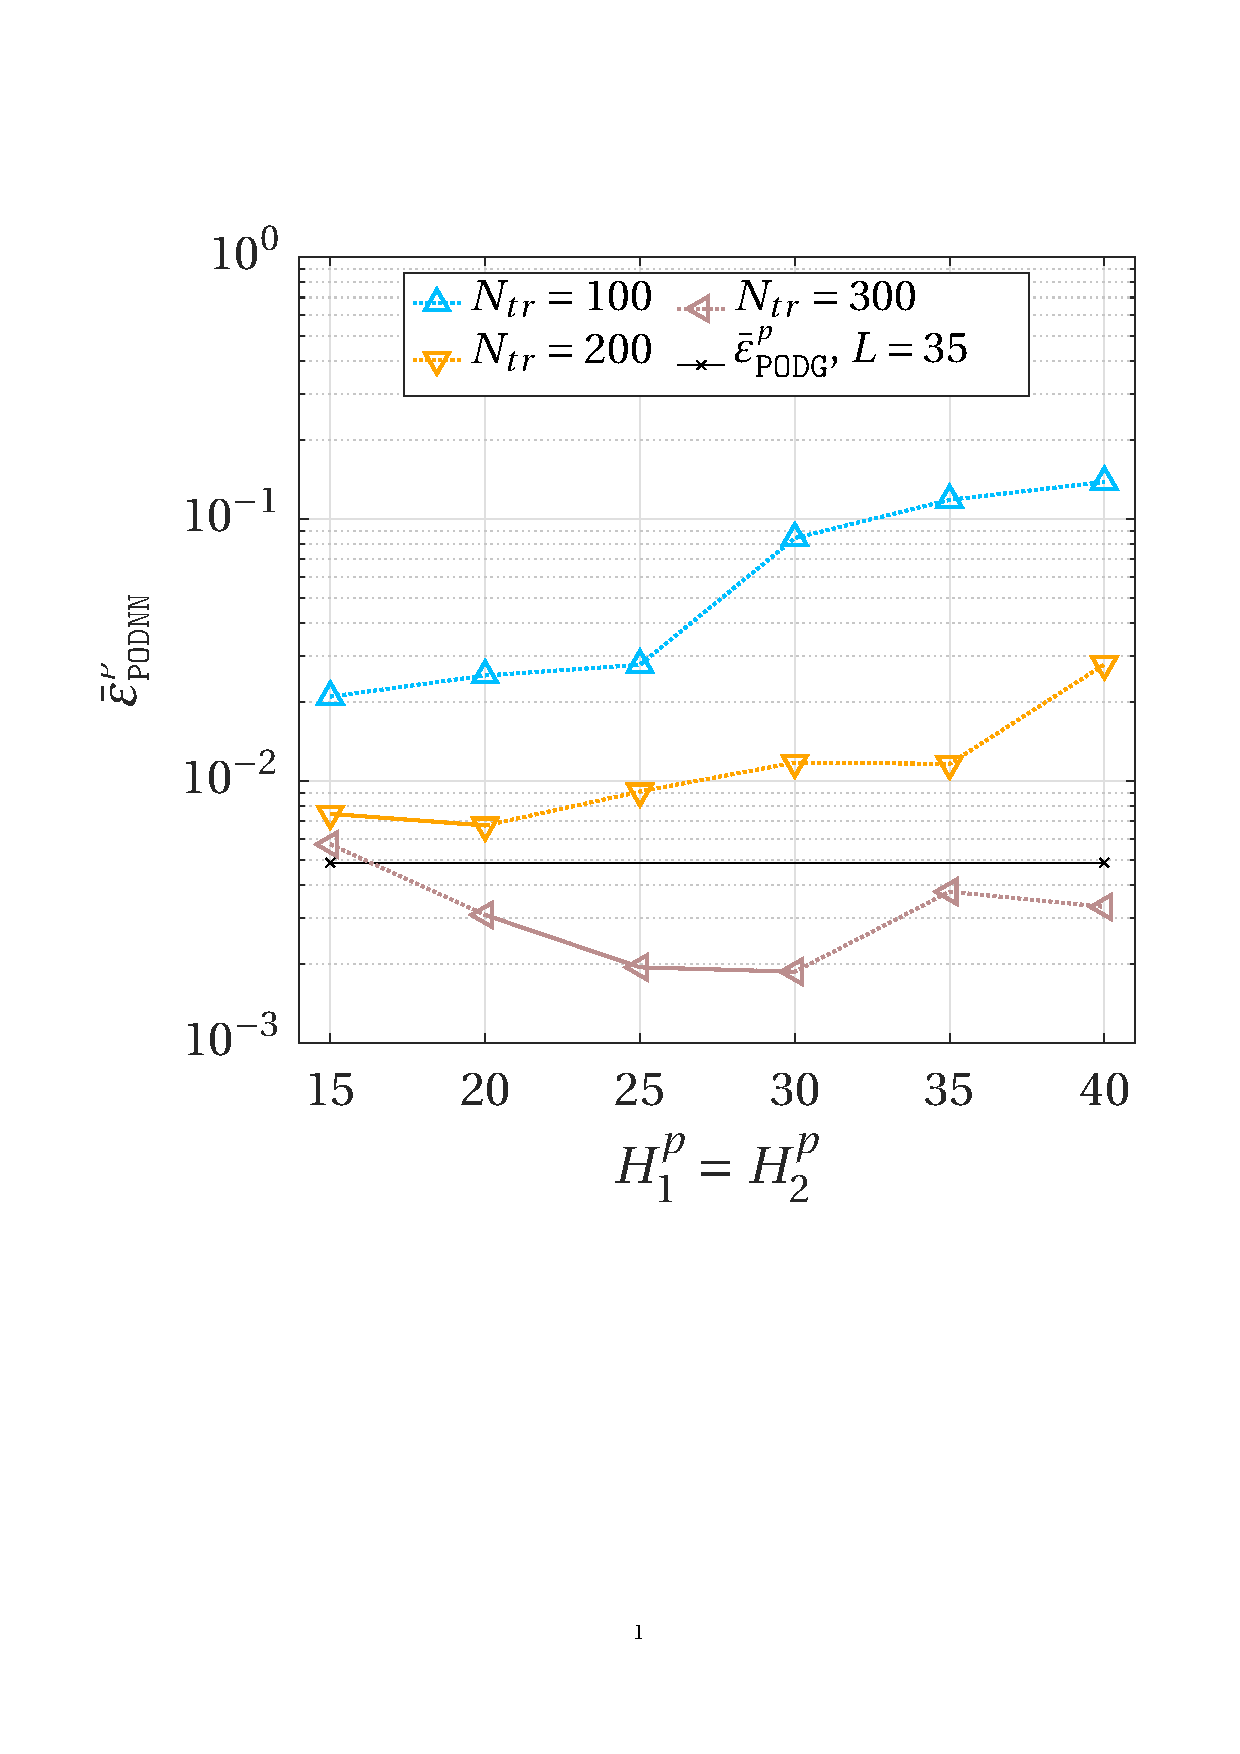
\includegraphics[scale = 0.37, trim = {1cm 9cm 1.5cm 3.5cm}, clip]{dc_200_p_nn_convergence}
			\hspace*{1cm}
			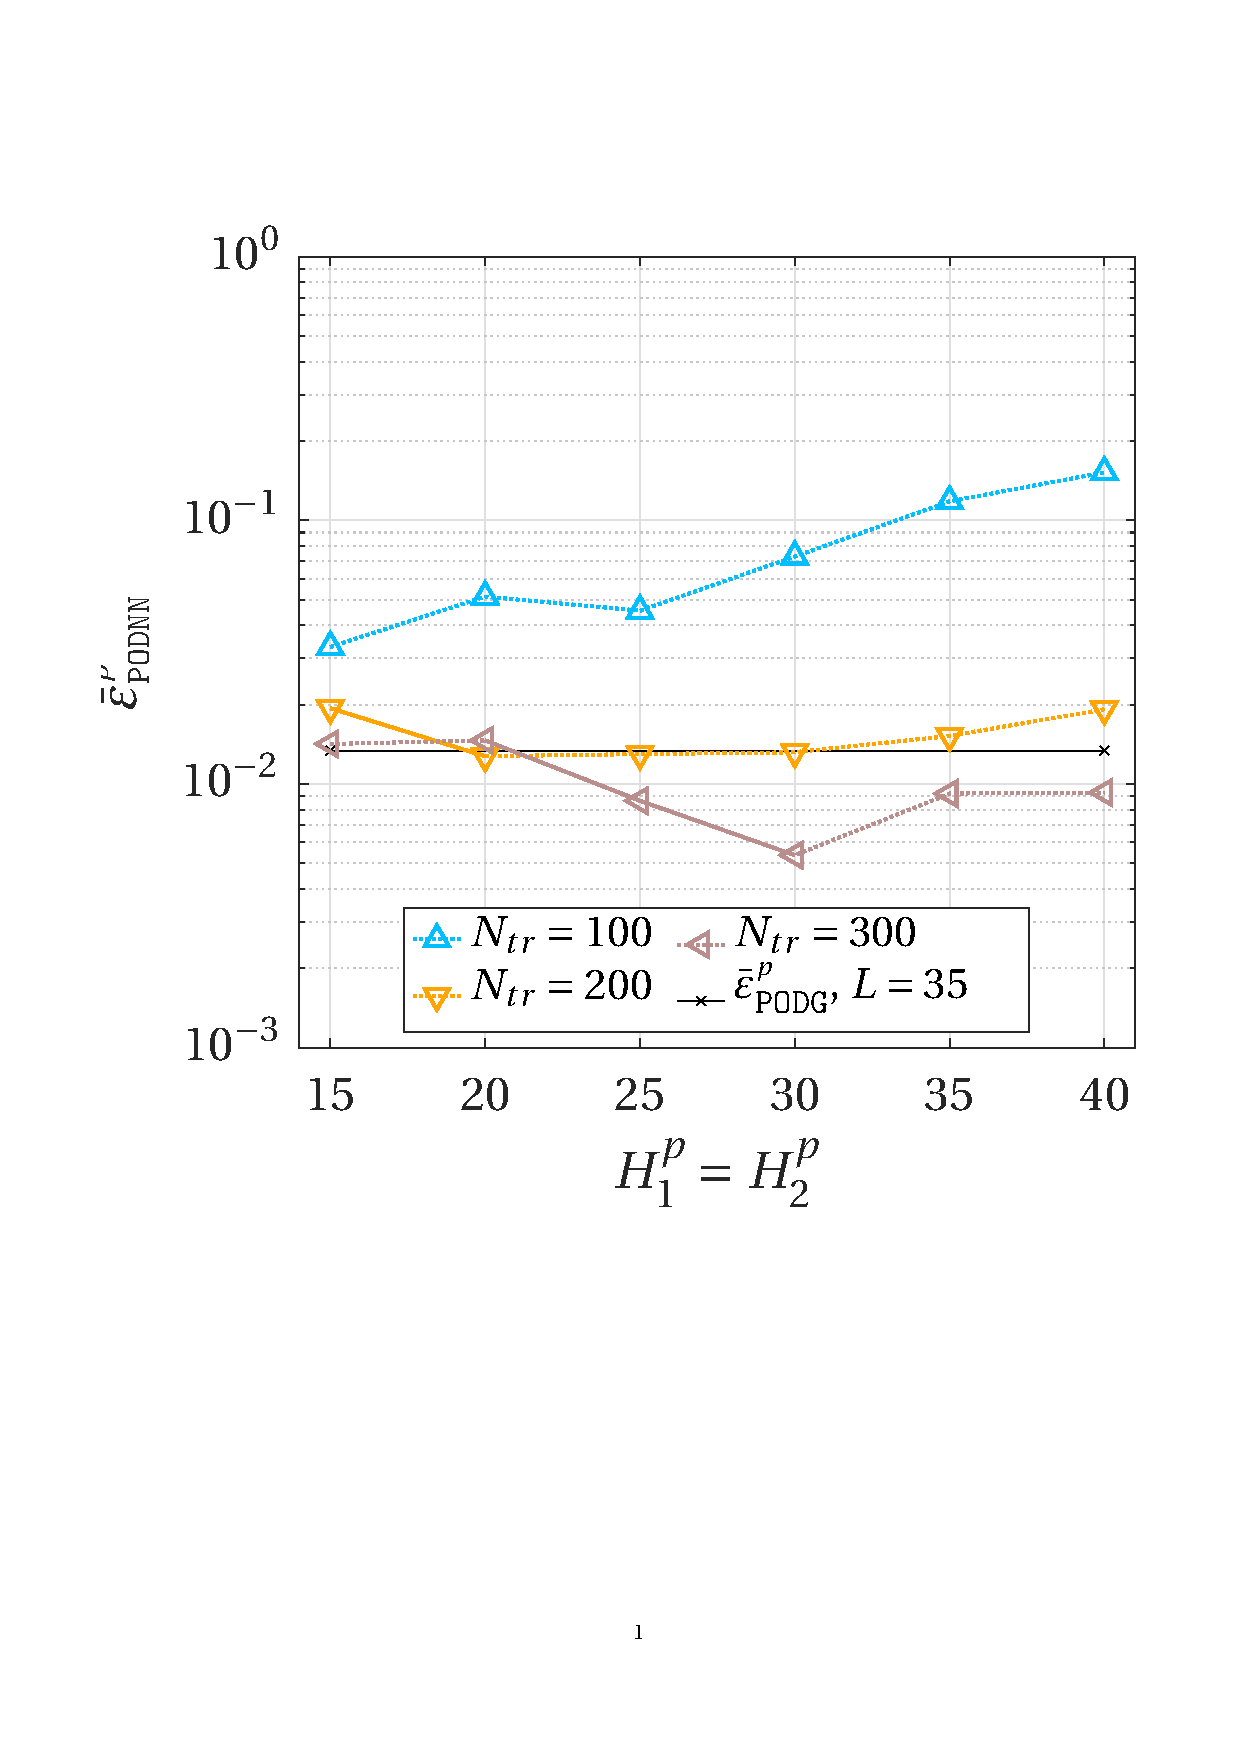
\includegraphics[scale = 0.37, trim = {1cm 9cm 1.5cm 3.5cm}, clip]{dc_400_p_nn_convergence}
			
			\vspace*{-0.1cm}
			
			\caption{Convergence analysis with respect to the number of hidden neurons and training samples used within the POD-NN procedure to approximate the velocity field (\textcolor{deepgreen}{\emph{top}}) and the pressure distribution (\textcolor{deepgreen}{\emph{bottom}}) by means of $35$ modal functions. The Reynold's number is either $200$ (\textcolor{deepgreen}{\emph{left}}) or $400$ (\textcolor{deepgreen}{\emph{right}}).}
			\label{fig:dc-nn-convergence}
		\end{figure}

		Figure \ref{fig:dc-error-vs-rank} reports the error committed by both RB procedures when approximating the velocity field (\textcolor{deepgreen}{\emph{top}}) and the pressure distribution (\textcolor{deepgreen}{\emph{bottom}}) by means of $L_{\bg{v}}$ velocity modes, $L_p$ pressure modes and, exclusively for the POD-Galerkin method, $L_{\bg{s}}$ supremizer modes, with $5 \leq L_{\bg{v}} = L_{\bg{s}} = L_p \leq 35$. The plots \textcolor{deepgreen}{on the left} refer to a Reynold's number of $200$, the ones \textcolor{deepgreen}{on the right} to a Reynold's number of $400$. Note that for clarity of illustration, the symbols denoting the projection, POD-G and POD-NN errors have been identified with a superscript (either $\bg{v}$ or $p$) recalling the state variable they refer to. 

		While the error yielded on the velocity field shows an almost perfect exponential decay with the number of POD modes included in the RB model, the POD-G method faces difficulties in providing a correct recovery of the pressure, already for $Re = 200$. Indeed, the corresponding error curve is not monotone, and generally is at least one order of magnitude above the projection error. Conversely, the POD-NN method attains a satisfactory predictive accuracy. The advantages of resorting to a neural network-based nonlinear regression coupled with POD are evident when the approximation is built upon a few basis functions, say $L_p < 20$. Moreover, the proposed routine recommends the use of fewer neurons to predict the POD coefficients for the pressure than for the velocity, thus resulting in a lighter perceptron. 
		
		This is confirmed also by Fig. \ref{fig:dc-nn-convergence}, which provides a sensitivity analysis of the predictive accuracy featured by the POD-NN method with respect to the amount of neurons and training samples used. Observe that for the pressure (\textcolor{deepgreen}{\emph{bottom}}), employing more than $30$ neurons within each hidden layer is counter-productive, both for $Re = 200$ (\textcolor{deepgreen}{\emph{left}}) and $Re = 400$ (\textcolor{deepgreen}{\emph{right}}). This assertion agrees with the peculiar role played by the pressure in the parametrized lid-driven cavity problem, with similar patterns featured across the entire parameter domain. 
		
		\begin{figure}[h!]
			\center
			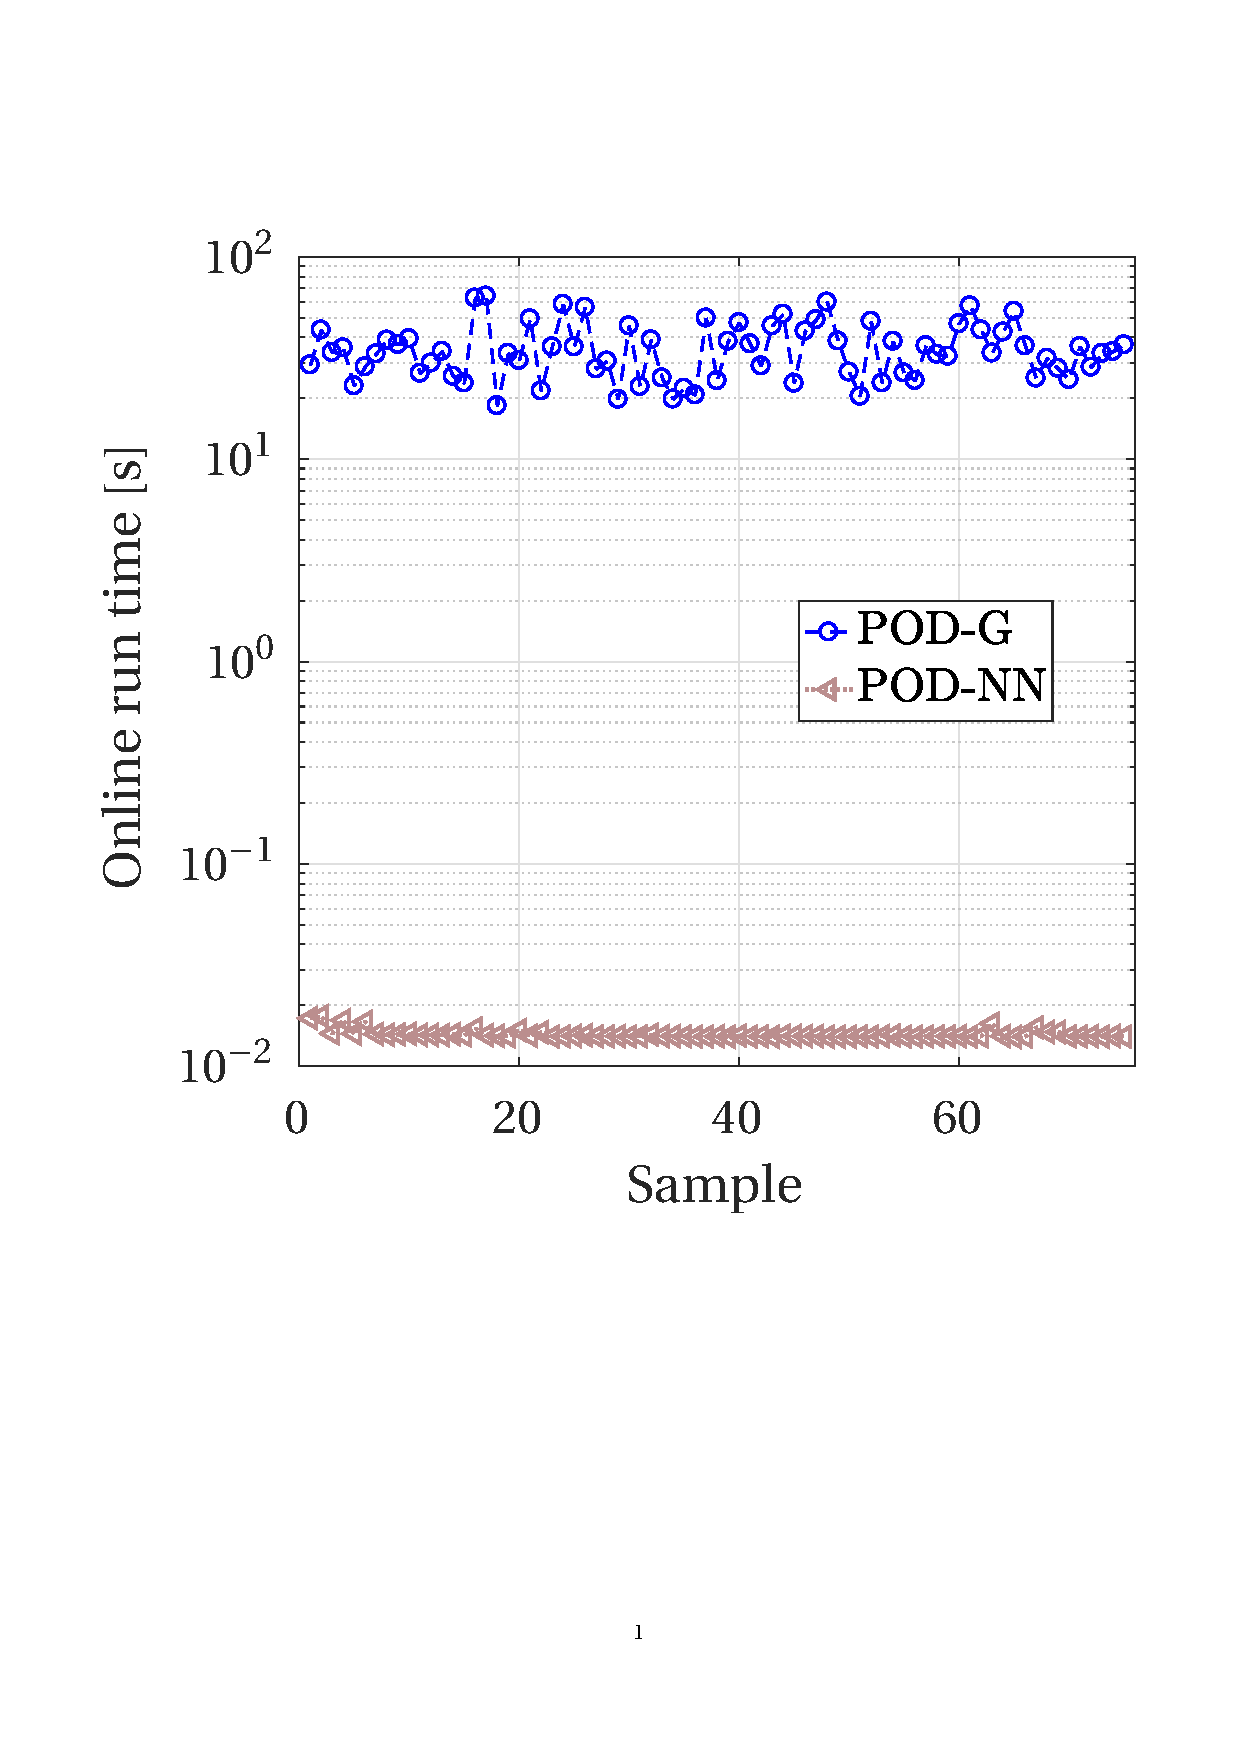
\includegraphics[scale = 0.37, trim = {1cm 9cm 1.5cm 3.5cm}, clip]{dc_200_time}
			\hspace*{0.6cm}
			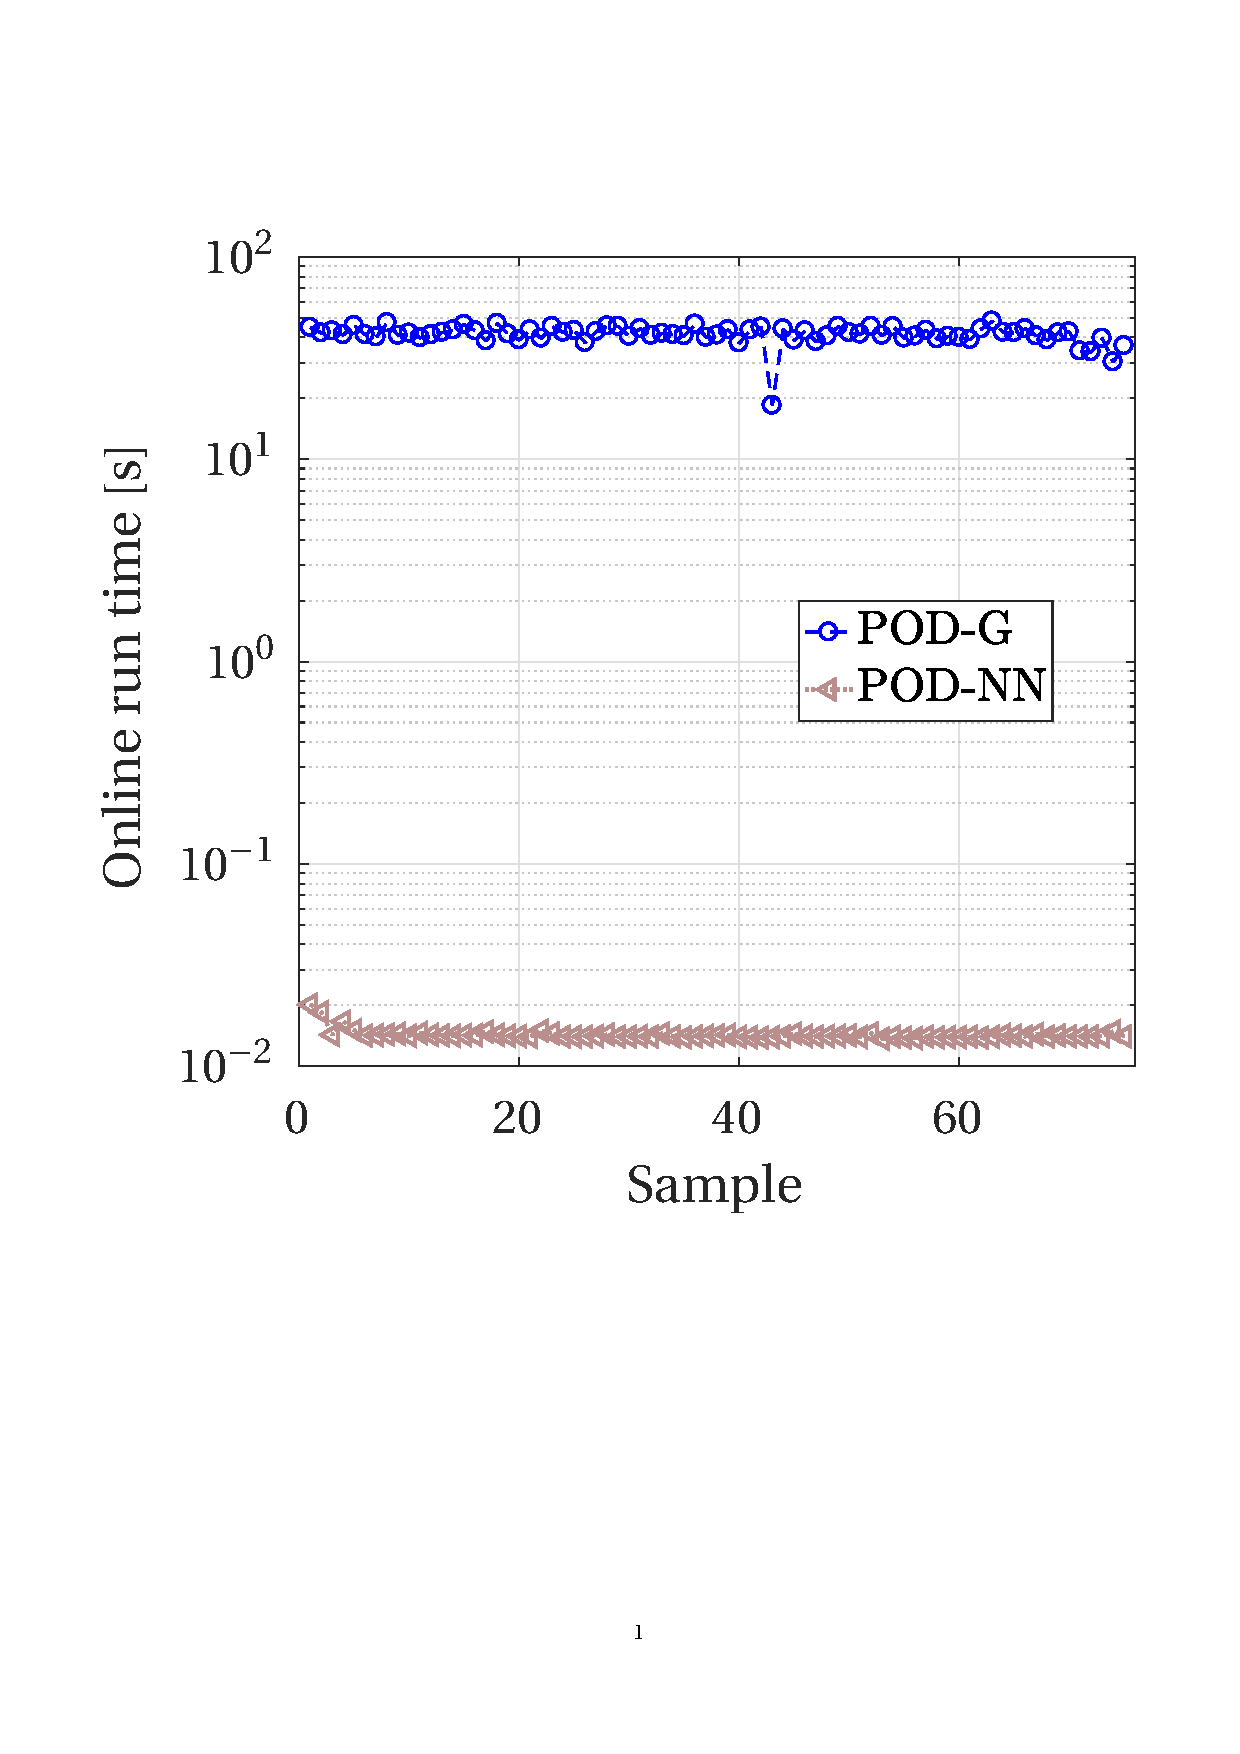
\includegraphics[scale = 0.37, trim = {1cm 9cm 1.5cm 3.5cm}, clip]{dc_400_time}
			
			\vspace*{-0.1cm}
			
			\caption{Online run times for the POD-G and the POD-NN method applied to the lid-driven cavity problem with $Re = 200$ (\emph{left}) and $Re = 400$ (\emph{right}). $N_{te} = 75$ test configurations are considered. For the POD-NN method, the reported times include the (sequential) evaluation of both neural networks for the velocity and pressure field.}
			\label{fig:dc-time}
			
			\vspace*{0.2cm}

			\center
			\hspace*{-0.7cm}
			\stackunder[-6pt]{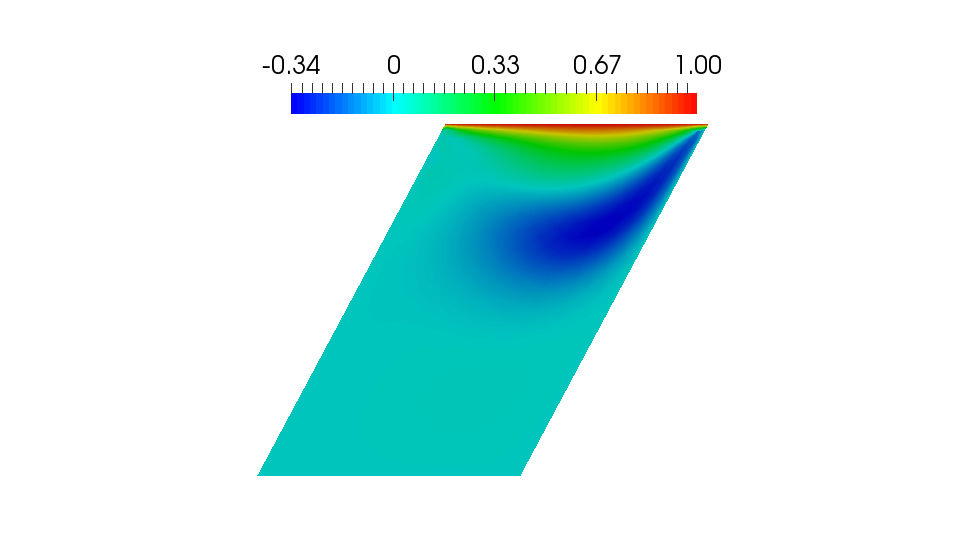
\includegraphics[scale = 0.22, trim = {7cm 0 7.5cm 0.4cm}, clip]{dc_400_fem_vx_1}}{\footnotesize{$\bg{\mu} = (1.12, \, 1.70, \, 1.08)$, FEM}}
			\hspace*{0.8cm}
			\stackunder[-6pt]{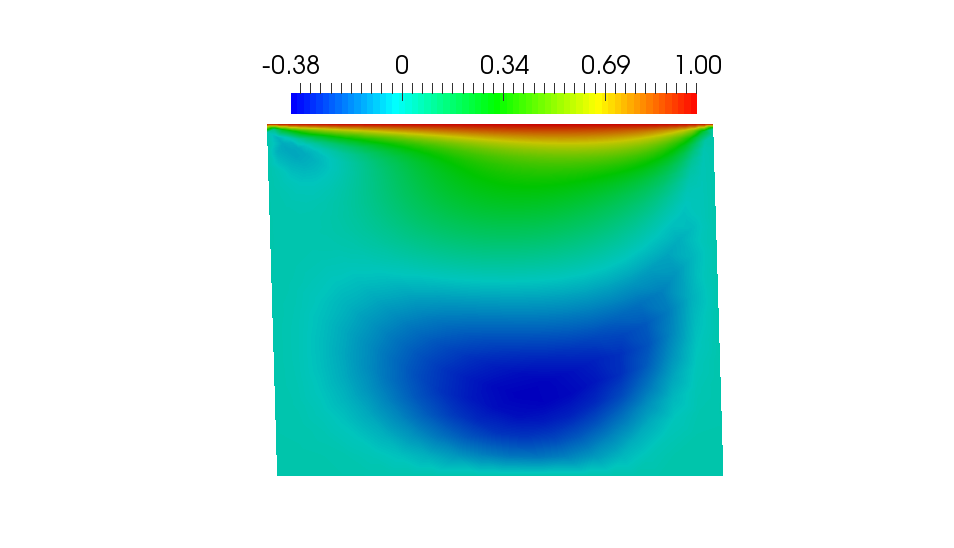
\includegraphics[scale = 0.22, trim = {8.25cm 0 7.5cm 0.4cm}, clip]{dc_400_fem_vx_2}}{\footnotesize{$\bg{\mu} = (1.90, \, 1.50, \, 1.60)$, FEM}}
			\hspace*{0.5cm}
			\stackunder[-6pt]{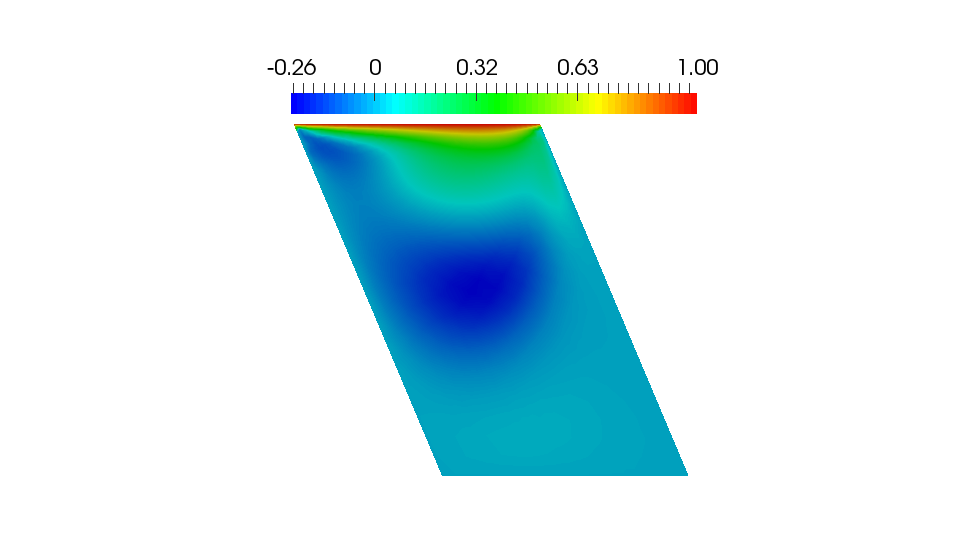
\includegraphics[scale = 0.22, trim = {4.5cm 0 3cm 0.4cm}, clip]{dc_400_fem_vx_3}}{\footnotesize{$\bg{\mu} = (1.78, \, 1.99, \, 2.29)$, FEM}} \\[0.4cm]
			
			\vspace*{-0.2cm}

			\hspace*{-0.7cm}
			\stackunder[-6pt]{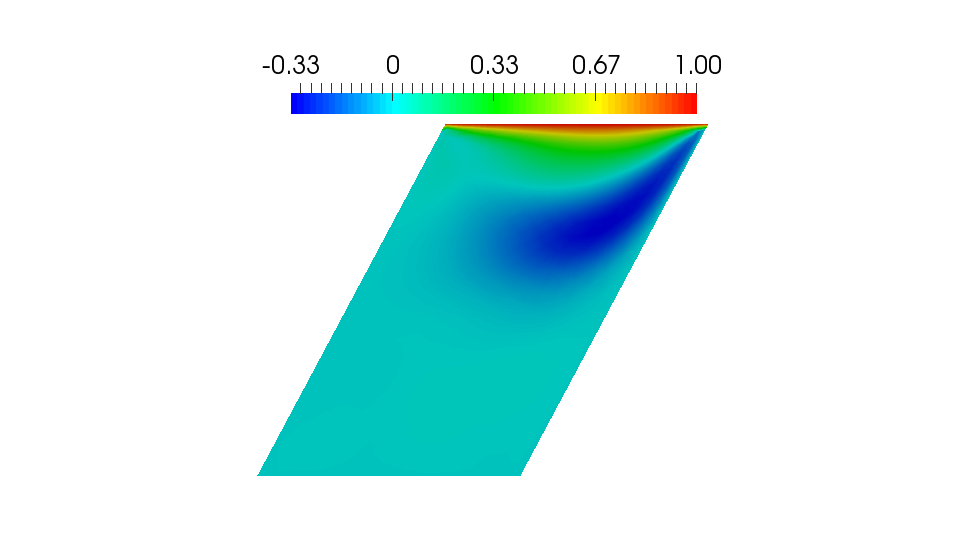
\includegraphics[scale = 0.22, trim = {7cm 0 7.5cm 0.4cm}, clip]{dc_400_podnn_vx_1}}{\footnotesize{$\bg{\mu} = (1.12, \, 1.70, \, 1.08)$, POD-NN}}
			\hspace*{0.8cm}
			\stackunder[-6pt]{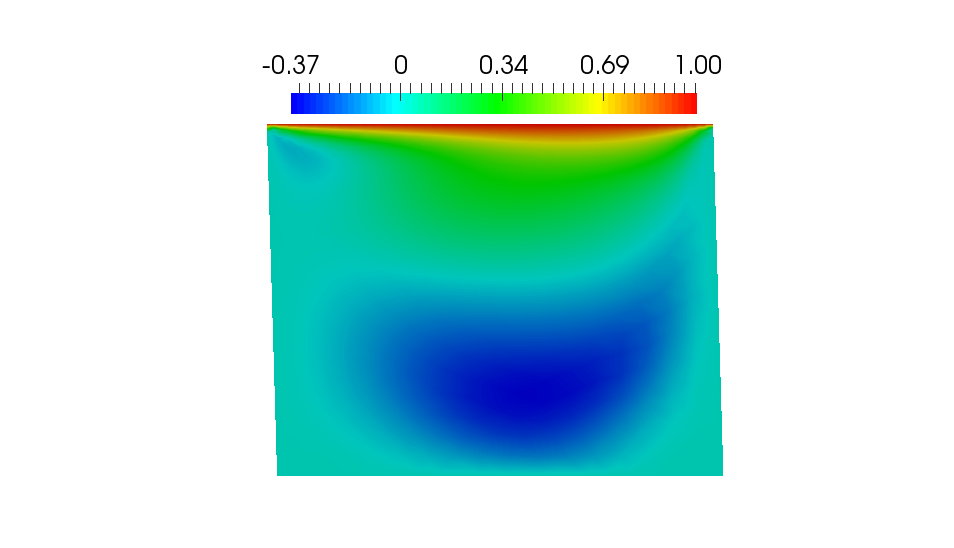
\includegraphics[scale = 0.22, trim = {8.25cm 0 7.5cm 0.4cm}, clip]{dc_400_podnn_vx_2}}{\footnotesize{$\bg{\mu} = (1.90, \, 1.50, \, 1.60)$, POD-NN}}
			\hspace*{0.5cm}
			\stackunder[-6pt]{\includegraphics[scale = 0.22, trim = {4.5cm 0 3cm 0.4cm}, clip]{dc_400_podnn_vx_3}}{\footnotesize{$\bg{\mu} = (1.78, \, 1.99, \, 2.29)$, POD-NN}}
			
			\caption{$\wt{x}$-velocity contour at three parameter values, as computed through the FE (\emph{top}) and POD-NN (\emph{bottom}) method. For each configuration, the Reynold's number is $400$.}
			\label{fig:dc-x-velocity}
		\end{figure}

		On the contrary, we have seen that the velocity field presents more complex dynamics, highly varying with the domain configuration. As a result, an optimal approximation of the velocity is obtained for the maximum values of $H_i^{\bg{v}}$, $i = 1, \, 2$, and $N_{tr}$ tested, that is, $H_1^{\bg{v}} = H_2^{\bg{v}} = 35$ and $N_{tr} = 300$ for $Re = 200$, $H_1^{\bg{v}} = H_2^{\bg{v}} = 40$ and $N_{tr} = 300$ for $Re = 400$. Moreover, we may not be able to exactly attain the same precision enabled by the standard POD-Galerkin procedure, although the results are quite similar. However, this (slight) loss of accuracy is offset by a (great) reduction in the online run time: the POD-NN method takes around $2/100$ of seconds per query, against the average $40$ seconds required by the POD-G method; see Fig. \ref{fig:dc-time}. As for the test cases for the Poisson problem, this comes at the cost of a longer offline phase.				
				
		Another numerical evidence of the predictive accuracy of the proposed POD-NN RB method is provided in Fig. \ref{fig:dc-x-velocity}, showing the contour plots for the $\wt{x}$-velocity computed through the FE (\emph{top}) and the POD-NN (\emph{bottom}) scheme. Three different configurations, corresponding to as many input vectors, are considered; the Reynold's number is fixed to $400$. We can appreciate good agreement between the solutions given by the full-order and the reduced order methods. 
														
		Lastly, Fig. \ref{fig:dc-streamlines} compares the streamlines obtained through the direct method (\emph{top}) and the proposed reduced basis approach (\emph{bottom}) over the three configurations previously considered. Streamlines provide an interesting test, as minor variations in velocity contours may lead to substantial differences in the streamlines \cite{Chen17}. Nevertheless, we observe a good agreement between the two methods. In particular, in the second example, the POD-NN method is still able to detect the two micro recirculation zones at the lower corners of the domain. On the other hand, the method partially fails in properly describing the velocity field at the bottom-left corner in the first configuration and at the bottom-right corner in the last configuration. However, these are effectively dead zones, and one can safely disregard these little imprecisions.
				
		\begin{figure}[t]
			\center
			
			\hspace*{-0.7cm}
			\stackunder[-6pt]{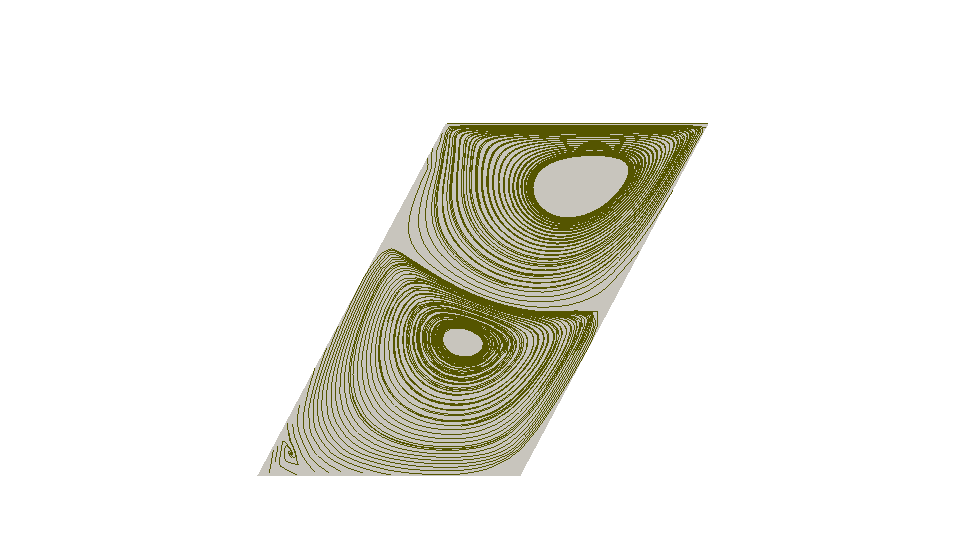
\includegraphics[scale = 0.22, trim = {7cm 0 7.5cm 0.4cm}, clip]{dc_400_fem_stream_1}}{\footnotesize{$\bg{\mu} = (1.12, \, 1.70, \, 1.08)$, FEM}}
			\hspace*{0.8cm}
			\stackunder[-6pt]{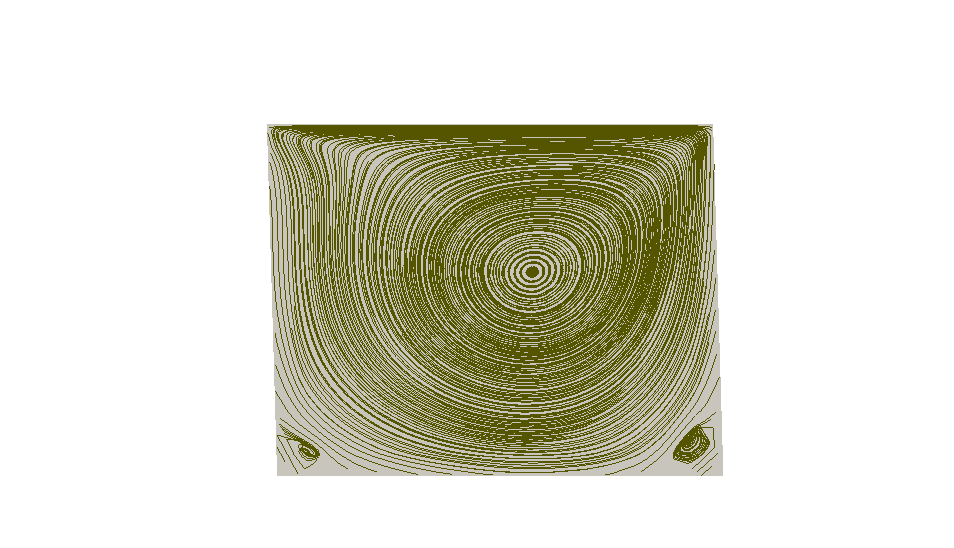
\includegraphics[scale = 0.22, trim = {8.25cm 0 7.5cm 0.4cm}, clip]{dc_400_fem_stream_2}}{\footnotesize{$\bg{\mu} = (1.90, \, 1.50, \, 1.60)$, FEM}}
			\hspace*{0.5cm}
			\stackunder[-6pt]{\includegraphics[scale = 0.22, trim = {4.5cm 0 3cm 0.4cm}, clip]{dc_400_fem_stream_3}}{\footnotesize{$\bg{\mu} = (1.78, \, 1.99, \, 2.29)$, FEM}} \\
			
			\hspace*{-0.7cm}
			\stackunder[-6pt]{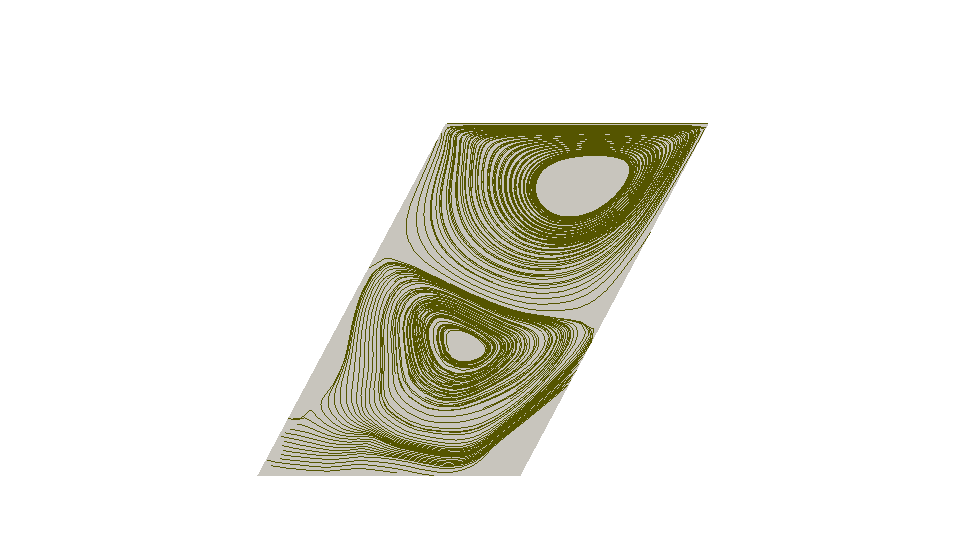
\includegraphics[scale = 0.22, trim = {7cm 0 7.5cm 2cm}, clip]{dc_400_podnn_stream_1}}{\footnotesize{$\bg{\mu} = (1.12, \, 1.70, \, 1.08)$, POD-NN}}
			\hspace*{0.8cm}
			\stackunder[-6pt]{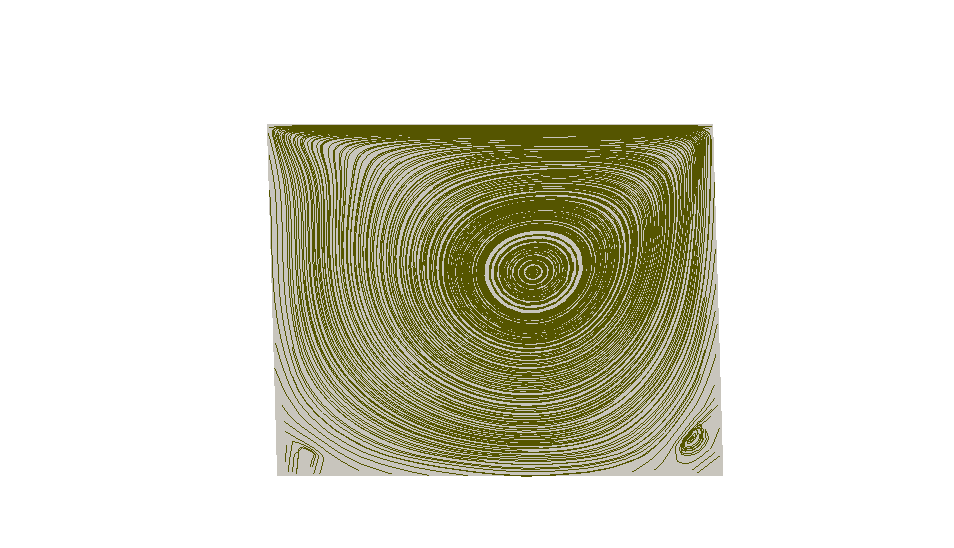
\includegraphics[scale = 0.22, trim = {8.25cm 0 7.5cm 2cm}, clip]{dc_400_podnn_stream_2}}{\footnotesize{$\bg{\mu} = (1.90, \, 1.50, \, 1.60)$, POD-NN}}
			\hspace*{0.5cm}
			\stackunder[-6pt]{\includegraphics[scale = 0.22, trim = {4.5cm 0 3cm 2cm}, clip]{dc_400_podnn_stream_3}}{\footnotesize{$\bg{\mu} = (1.78, \, 1.99, \, 2.29)$, POD-NN}}
			
			\caption{Streamlines at three parameter values, as computed through the FE (\emph{top}) and POD-NN (\emph{bottom}) method. For each configuration, the Reynold's number is $400$.}
			\label{fig:dc-streamlines}
		\end{figure}
	
	
	%
	% Section 7 : Conclusion
	%
	
	\section{Conclusion}
	\label{section:Conclusion}	
	
		In this work, we propose a non-intrusive RB method (referred to as POD-NN) for parametrized steady-state PDEs. The method extracts a reduced basis from a collection of snapshots through a POD procedure and employs multi-layer perceptrons to approximate the coefficients of the reduced model. By exploiting the fundamental results by Cybenko (see Subsection \ref{section:Network topology}), we limit ourselves to perceptrons endowed with two hidden layers. The identification of the optimal number of inner neurons and the minimum amount of training samples to prevent overfitting is performed during the offline stage through an automatic routine, relying upon the latin hypercube sampling and the Levenberg-Marquardt training algorithm. On the one hand, this guarantees a complete decoupling between the offline and the online phase, with the latter having a computational cost independent of the dimension of the full-order model. On the other hand, this extends the offline stage with respect to a standard projection-based RB procedure, making the POD-NN method practically convenient only when the underlying PDE has to be solved for many parameter values (many-query context). 		

		The POD-NN method has been successfully tested on the nonlinear Poisson equation in one and two spatial dimensions, and on two-dimensional cavity viscous flows, modeled through the steady incompressible Navier-Stokes equations. In particular, the proposed RB strategy enables the same predictive accuracy provided by the POD-Galerkin method while reducing the CPU time required to process an online query by two or even three order of magnitudes.		

		All test cases considered in our numerical studies involved three parameters, affecting either physical or geometrical factors of the differential problem. The extension of the POD-NN method to time-dependent problems depending on many parameters is left as future work. 		

		Lastly, let us point out that although in this work we used POD to recover a reduced space, this choice is not binding, and a greedy approach may also be pursued. 
		
	
	%
	% Bibliography
	%
		
	\section*{References}
		
	\begin{thebibliography}{50}
		
		\bibitem{Ams10}
		Amsallem., D. (2010). \emph{Interpolation on manifolds of CFD-based fluid and finite element-based structural reduced-order models for on-line aeroelastic predictions}. Doctoral dissertation, Department of Aeronautics and Astronautics, Stanford University.
		
		\bibitem{Bal14}
		Ballarin, F., Manzoni, A., Quarteroni, A., Rozza, G. (2014). \emph{Supremizer stabilization of POD-Galerkin approximation of parametrized Navier-Stokes equations}. MATHICSE Technical Report, \'Ecole Polytechnique F\'ed\'erale de Lausanne.
	
		\bibitem{Bar04}
		Barrault, M., Maday, Y., Nguyen, N. C., Patera, A. T. (2004). \emph{An 'empirical interpolation' method: Application to efficient reduced-basis discretization of partial differential equations}. Comptes Rendus Mathematique, 339(9):667-672.
		
		\bibitem{BNR00}
		Barthelmann, V., Novak, E., Ritter, K. (2000). \emph{High-dimensional polynomial interpolation on sparse grids}. Advances in Computational Mathematics, 12(4):273-288.
		
		\bibitem{Ben04}
		Bends\o{}e, M. P., Sigmund, O. (2004). \emph{Topology optimization: Theory, methods and applications}. Heidelberg, DE: Springer Science \& Business Media. 
		
		\bibitem{Bro93}
		Brown, P. F., Pietra, V. J. D., Pietra, S. A. D., Mercer, R. L. (1993). \emph{The mathematics of statistical machine translation: Parameter estimation}. Computational linguistics, 19(2):263-311.
		
		\bibitem{Buf12}
		Buffa, A., Maday, Y., Patera, A. T., Prud'Homme, C., Turinici, G. (2012). \emph{A priori convergence of the greedy algorithm for the parametrized reduced basis method}. ESAIM: Mathematical Modelling and Numerical Analysis, 46:595-603.
		
		\bibitem{Bur06}
		Burkardt, J., Gunzburger, M., Lee, H. C. (2006). \emph{POD and CVT-based reduced-order modeling of Navier-Stokes flows}. Computer Methods in Applied Mechanics and Egninnering, 196:337-355.
		
		\bibitem{Cas15}
		Casenave, F., Ern, A., Lelièvre, T. (2015). \emph{A nonintrusive reduced basis method applied to aeroacoustic simulations}. Advances in Computational Mathematics, 41:961-986.
		
		\bibitem{Cha10}
		Chaturantabut, S., Sorensen, D. C. (2010). \emph{Nonlinear model reduction via discrete empirical interpolation}. SIAM Journal on Scientific Computing, 32(5):2737-2764.
		
		\bibitem{Chen17}
		Chen, W., Hesthaven, J. S., Junqiang, B., Yang, Z., Tihao, Y. (2017). \emph{A greedy non-intrusive reduced order model for fluid dynamics}. Submitted to American Institute of Aeronautics and Astronautics.
	
		\bibitem{Cyb88}
		Cybenko, G. (1988). \emph{Continuous valued neural networks with two hidden layers are sufficient}. Technical Report, Department of Computer Science, Tufts University.
		
		\bibitem{Cyb89}
		Cybenko, G. (1989). \emph{Approximation by superpositions of a sigmoidal function}. Mathematics of Control, Signals, and Systems, 2(4):303–314.
		
		\bibitem{Deb78}
		De Boor, C. (1978). \emph{A practical guide to splines}. New York, NY: Springer-Verlag.
		
		\bibitem{Dep08}
		Deparis, S. (2008). \emph{Reduced basis error bound computation of parameter-dependent Navier-Stokes equations by the natural norm approach}. SIAM Journal of Numerical Analysis, 46(4):2039-2067.
		
		\bibitem{Dho14}
		Dhondt, G. (2014). \emph{CalculiX CrunchiX user's manual}. Available at \url{http://web.mit.edu/calculix_v2.7/CalculiX/ccx_2.7/doc/ccx/node1.html}.
		
		\bibitem{EY36}
		Eckart, C., Young, G. (1936). \emph{The approximation of one matrix by another of lower rank}. Psychometrika, 1:211-218.
		
		\bibitem{Eft08}
		Eftang, J. L. (2008). \emph{Reduced basis methods for partial differential equations}. Master thesis, Department of Mathematical Sciences, Norwegian University of Science and Technology.
		
		\textcolor{deepgreen}{
			\bibitem{GMW81}
			Gill, P. E., Murray, W., Wright, M. H. (1981). \emph{Practical optimization}. Academic Press.
		}

		\bibitem{Hag94}
		Hagan, M. T., Menhaj, M. B. (1994). \emph{Training feedforward networks with the Marquardt algorithm}. IEEE Transactions on Neural Networks, 5(6):989-993.
		
		\bibitem{Hag96}
		Hagan, M. T., Demuth, H. B., Beale, M. H. (1996). \emph{Neural Network Design}. Boston, MA: PWS Publishing.		

		\bibitem{Hay05}
		Haykin, S. (2004). \emph{Neural Networks: A comprehensive foundation}. Upper Saddle River, NJ: Prentice Hall.
		
		\bibitem{HSR16}
		Hesthaven, J. S., Stamn, B., Rozza, G. (2016). \emph{Certified reduced basis methods for parametrized partial differential equations}. New York, NY: Springer.
		
		\bibitem{HSZ14}
		Hesthaven, J. S., Stamn, B., Zhang, S. (2014). \emph{Efficienty greedy algorithms for high-dimensional parameter spaces with applications to empirical interpolation and reduced basis methods}. ESAIM: Mathematical Modelling and Numerical Analysis, 48(1):259-283.
		
		\bibitem{Imam08}
		Imam, R. L. (2008). \emph{Latin hypercube sampling}. Encyclopedia of Quantitative Risk Analysis and Assessment.
		
		\bibitem{JIR14}
		Jaggli, C., Iapichino, L., Rozza, G. (2014). \emph{An improvement on geometrical parametrizations by transfinite maps}. Comptes Rendus de l'Acad\'emie des Sciences Paris, Series I, 352:263-268. 
				
		\bibitem{Koh95}
		Kohavi, R. (1995). \emph{A study of cross-validation and bootstrap for accuracy estimation and model selection}. Proceedings of the $40^{th}$ International Joint Conference on Artificial Intelligence, 2(12):1137-1143.
		
		\bibitem{Kri07}
		Kriesel, D. (2007). \emph{A Brief Introduction to Neural Networks}. Retrieved from \url{http://www.dkriesel.com/en/science/neural_networks}.
		
		\bibitem{LeM10}
		Le Ma\^{i}tre, O., Knio, O. M. (2010). \emph{Spectral methods for uncertainty quantification with applications to computational fluid dynamics}. Berlin, DE: Springer Science \& Business Media.
		
		\textcolor{deepgreen}{
			\bibitem{Lev44}
			Levenberg, K. (1944). \emph{A method for the solution of certain non-linear problems in least squares}. Quarterly of Applied Mathematics, 2:164-168.
		}

		\bibitem{LM67}
		Lee, E. B., Markus, L. (1967). \emph{Foundations of optimal control theory}. New York, NY: John Wiley \& Sons.
		
		\bibitem{Lia02}
		Liang, Y. C., Lee, H. P., Lim, S. P., Lin, W. Z., Lee, K. H., Wu, C. G. (2002) \emph{Proper orthogonal decomposition and its applications - Part I: Theory}. Journal of Sound and Vibration, 252(3):527-544.

		\bibitem{Mad06}
		Maday, Y. (2006) \emph{Reduced basis method for the rapid and reliable solution of partial differential equations}. Proceedings of the International Congress of Mathematicians, Madrid, Spain, 1255-1269.
		
		\bibitem{Mar63}
		Marquardt, D. W. (1963). \emph{An algorithm for least-squares estimation of nonlinear parameters}. Journal of the Society for Industrial and Applied Mathematics, 11(2):431-441.
		
		\bibitem{Mat16}
		The MathWorks, Inc. (2016). \emph{Machine learning challenges: Choosing the best model and avoiding overfitting}. Retrieved from \url{https://it.mathworks.com/campaigns/products/offer/common-machine-learning-challenges.html}.
		
		\bibitem{MM10}
		Mitchell, W., McClain, M. A. (2010). \emph{A collection of 2D elliptic problems for testing adaptive algorithms}. NISTIR 7668.
		
		\bibitem{MN16}
		Manzoni, A., Negri, F. (2016). \emph{Automatic reduction of PDEs defined on domains with variable shape}. MATHICSE technical report, \'Ecole Polytechnique F\'ed\'erale de Lausanne.
		
		\textcolor{deepgreen}{
			\bibitem{Mol93}
			M\o{}ller, M. D. (1993). \emph{A scaled conjugate gradient algorithm for fast supervised learning}. Neural Networks, 6:525-533.
		}

		\bibitem{Nie15}
		Nielsen, M. A. (2015). \emph{Neural Networks and Deep Learning}. Determination Press.
				
		\bibitem{NMA15}
		Negri, F., Manzoni, A., Amsallem, D. (2015). \emph{Efficient model reduction of parametrized systems by matrix discrete empirical interpolation}. Journal of Computational Physics, 303:431-454.
		
		\bibitem{Per02}
		Persson, P. O. (2002). \emph{Implementation of finite-element based Navier-Stokes solver}. Massachussets Institue of Technology.
		
		\bibitem{Pru02}
		Prud'homme, C., Rovas, D. V., Veroy, K., Machiels, L., Maday, Y., Patera, A. T., Turinici, G. (2002). \emph{Reliable real-time solution of parametrized partial differential equations: Reduced-basis output bound methods}. Journal of Fluids Engineering, 124(1):70-80.
		
		\bibitem{Qua10}
		Quarteroni, A. (2010). \emph{Numerical models for differential problems} (Vol. 2). New York, NY: Springer Science \& Business Media.
		
		\bibitem{QMN15}
		Quarteroni, A., Manzoni, A., Negri, F. (2015). \emph{Reduced basis methods for partial differential equations: An introduction} (Vol. 92). New York, NY: Springer, 2015.
		
		\bibitem{Ran99}
		Rannacher, R. (1999). \emph{Finite element methods for the incompressible Navier-Stokes equations}. Lecture notes, Institute of Applied Mathematics, University of Heidelberg.
		
		\bibitem{Ros58}
		Rosenblatt, F. (1958). \emph{The perceptron: A probabilistic model for information storage and organization in the brain}. Psychological Review, 65:386-408.
		
		\bibitem{Sch07}
		Schmidt, E. (1907). \emph{Zur theorie der linearen und nichtlinearen integralgleichungen. I. Teil: Entwicklung willk\"urlicher funktionen nach systemen vorgeschriebener}. Mathematische Annalen, 63:433-476.
		
		\bibitem{SD13}
		Stergiou, C., Siganos, D. (2013). \emph{Neural Networks}. Retrieved from \url{https://www.doc.ic.ac.uk/~nd/surprise_96/journal/vol4/cs11/report.html#Introduction to neural networks}.
		
		\bibitem{Vol08}
		Volkwein, S. (2008). \emph{Model reduction using proper orthogonal decomposition}. Lecture notes, Department of Mathematics, University of Konstanz.
	\end{thebibliography}
	
\end{document}
